\documentclass{beamer}
% \usepackage[retainorgcmds]{IEEEtrantools}
% 
% \setbeamertemplate{enumerate items}[ball]

\usepackage[utf8x]{inputenc}
\usepackage{beamerthemeSzeged}
\usecolortheme{dolphin} %blueaggressive
% \usecolortheme{beaver} %redaggressive
\usepackage{graphicx}
\usepackage[font={scriptsize,it}]{caption}
\captionsetup[figure]{labelformat=empty}
\usepackage{graphics, setspace}
\usepackage{subfigure}
\usepackage{epsfig}
\usepackage{tikz}
\mode<presentation>{}
\usepackage{bibentry}
\usepackage{multicol}
\usepackage{mathtools}
\usepackage{amssymb}

\usepackage{amsmath,empheq}
\usepackage{xcolor}

\setbeamerfont{title}{family=\rm}
\setbeamercovered{transparent}

\let\oldfootnotesize\footnotesize
\renewcommand*{\footnotesize}{\oldfootnotesize\tiny}
% \usefonttheme{professionalfonts} % using non standard fonts for beamer
% \usefonttheme{structurebold} % default family is serif
%\usepackage{fontspec}
%\setmainfont{Liberation Serif}
%\input{psfig}
\newenvironment{variableblock}[3]{%
  \setbeamercolor{block body}{#2}
  \setbeamercolor{block title}{#3}
  \begin{block}{#1}}{\end{block}}
  
\makeatletter
\setbeamertemplate{footline}
{%
\begin{beamercolorbox}[colsep=1.0pt]{upper separation line foot}
  \end{beamercolorbox}
  \vspace{1pt}
    \hbox{%
    \begin{beamercolorbox}[wd=0.3333\textwidth,  ht=2.5ex, dp=1.125ex]{title in head/foot}%
      \flushleft\usebeamerfont{title in head/foot}\footnotesize \hspace{1pt} Internally Coupled Ears%\insertshorttitle
    \end{beamercolorbox}%
    \begin{beamercolorbox}[wd=0.67\textwidth, ht=2.5ex, dp=1.125ex, center]{title in head/foot}%
      \flushright\usebeamerfont{title in head/foot}\insertframenumber/\inserttotalframenumber\hspace*{2ex}
    \end{beamercolorbox}}
     \begin{beamercolorbox}[colsep=1.0pt]{lower separation line foot}
  \end{beamercolorbox}
}

\setbeamertemplate{headline}
{%
  \begin{beamercolorbox}[ht=3.5ex,dp=1.125ex,%
      leftskip=.3cm,rightskip=.3cm plus1fil]{section in head/foot}
    \usebeamerfont{section in head/foot}\usebeamercolor[fg]{section in head/foot}%
    \flushleft\small\insertsectionnavigationhorizontal{\textwidth}{\hskip0pt plus1fill}{\hskip0pt plus1fill}
    %\insertsectionhead
  \end{beamercolorbox}%
  \begin{beamercolorbox}[colsep=1.5pt]{middle separation line head}
  \end{beamercolorbox}
  \begin{beamercolorbox}[ht=2.5ex,dp=1.125ex,%
    leftskip=.3cm,rightskip=.3cm plus1fil]{subsection in head/foot}
    \usebeamerfont{subsection in head/foot}\insertsubsectionhead %\ - \insertsubsubsectionhead
  \end{beamercolorbox}%
  \begin{beamercolorbox}[colsep=1.5pt]{lower separation line head}
  \end{beamercolorbox}
}

\setbeamertemplate{blocks}[rounded][shadow=false]
\addtobeamertemplate{block begin}{\pgfsetfillopacity{0.8}}{\pgfsetfillopacity{1}}
\setbeamercolor*{block title example}{fg=blue!75,bg= blue!10}
\setbeamercolor*{block body example}{fg= black,bg= blue!5}
\setbeamercolor{frametitle}{fg=blue}
\beamertemplatenavigationsymbolsempty

\setbeamertemplate{section in toc}{$\bullet$ \normalsize\inserttocsection}
\setbeamertemplate{subsection in toc}{\hspace*{9pt}\small$\bullet$ \inserttocsubsection\\}
\makeatother

\title{\Large Mechanical Processing in Internally Coupled Ears}
\author{Anupam Prasad Vedurmudi}
\date{TMP Thesis Defence\\ \today}

\titlegraphic{\vspace{.1cm}\flushleft 
\includegraphics[width=.85cm]{Diagrams/T35logo2.png}\hspace*{8.3cm}~%
   
\includegraphics[width=2cm]{Diagrams/tmplogo.jpg}
}

% \AtBeginSection[]
% {
%   \begin{frame}<beamer>
%     \frametitle{Outline for Section \thesection}
%     \begin{multicols}{2}
%     \tableofcontents[currentsection,subsubsectionstyle=show/shaded]
%     \end{multicols}
%   \end{frame}
% }

\usefonttheme[onlymath]{serif}
% \titlegraphic{\vspace{8cm}}
\begin{document}

\begin{frame}[t]
%    \tikz [remember picture,overlay]
%     \node at
%         ([yshift=3cm]current page.south) 
%         %or: (current page.center)
%         {\includegraphics[width=\textwidth,height=.5\textheight]{someimage}};
   %\titlepage
 \titlepage
 \bibliographystyle{ieeetr}
\nobibliography{literatur}

\end{frame}

  \begin{frame}<beamer>
    \frametitle{Outline}
    \begin{multicols}{2}
    \tableofcontents
    \end{multicols}
  \end{frame}
%\logo{
\includegraphics[height=0.8cm]{Diagrams/T35logo2.png}\vspace{220pt}}

\section{Introduction}
\subsection{Auditory Systems}
\begin{frame}[t]
\frametitle{Auditory Systems}

 \begin{columns}
 
      \onslide<1>{\begin{column}{0.5\textwidth}
    \centering
    \includegraphics<1>[width = 1.5 cm]{Diagrams/Presentation/indepears.png}\\
    \end{column}}
     
   \onslide<2>{\begin{column}{0.5\textwidth}
    \centering
    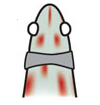
\includegraphics[width = 1.5 cm]{Diagrams/Presentation/coupledears.png}\\
    \end{column}}
    
  \end{columns}
  
 \onslide<1>{\begin{columns}
     \begin{column}{0.5\textwidth}
    \centering
    \underline{\textbf{Independent Ears}}
    \end{column}}
     
    \begin{column}{0.5\textwidth}
    \centering
    \underline{\textbf{Coupled Ears}}
    \end{column}
  \end{columns}

  \onslide<1>{\begin{columns}
    \begin{column}{0.5\textwidth}
    \centering
%     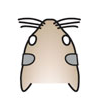
\includegraphics[width = 1.5 cm]{Diagrams/Presentation/indepears.png}\\
%     \underline{\textbf{Independent Ears}}
    \small
     \begin{itemize}
     \item[]
    \item[] Eustachian tubes generally very narrow.
     \item[] Effectively independent eardrum vibrations.
     \item[$\bullet$] eg. Mammals.
     \end{itemize}
    \end{column}}
     
    \begin{column}{0.5\textwidth}
    \centering
%     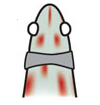
\includegraphics[width = 1.5 cm]{Diagrams/Presentation/coupledears.png}\\
%     \underline{\textbf{Coupled Ears}}
    \small
     \begin{itemize}
         \item[] Wide eustachian tubes open into the mouth cavity.
     \item[] Eardrums vibrations influence eachother.
     \item[$\bullet$] eg. \textbf<2>{Lizards}, birds, frogs.
     \end{itemize}
    \end{column}
    
  \end{columns}
\end{frame}

\subsection{Sound Localization}
\begin{frame}[t]
 \frametitle{Localization - Independent Ears}
 %Localization using frequency dependent phase and amplitude differences between the ears.
 %\vspace{\baselineskip}
  
 \begin{columns}
 
      \onslide<1->{\begin{column}{0.5\textwidth}
    \centering
    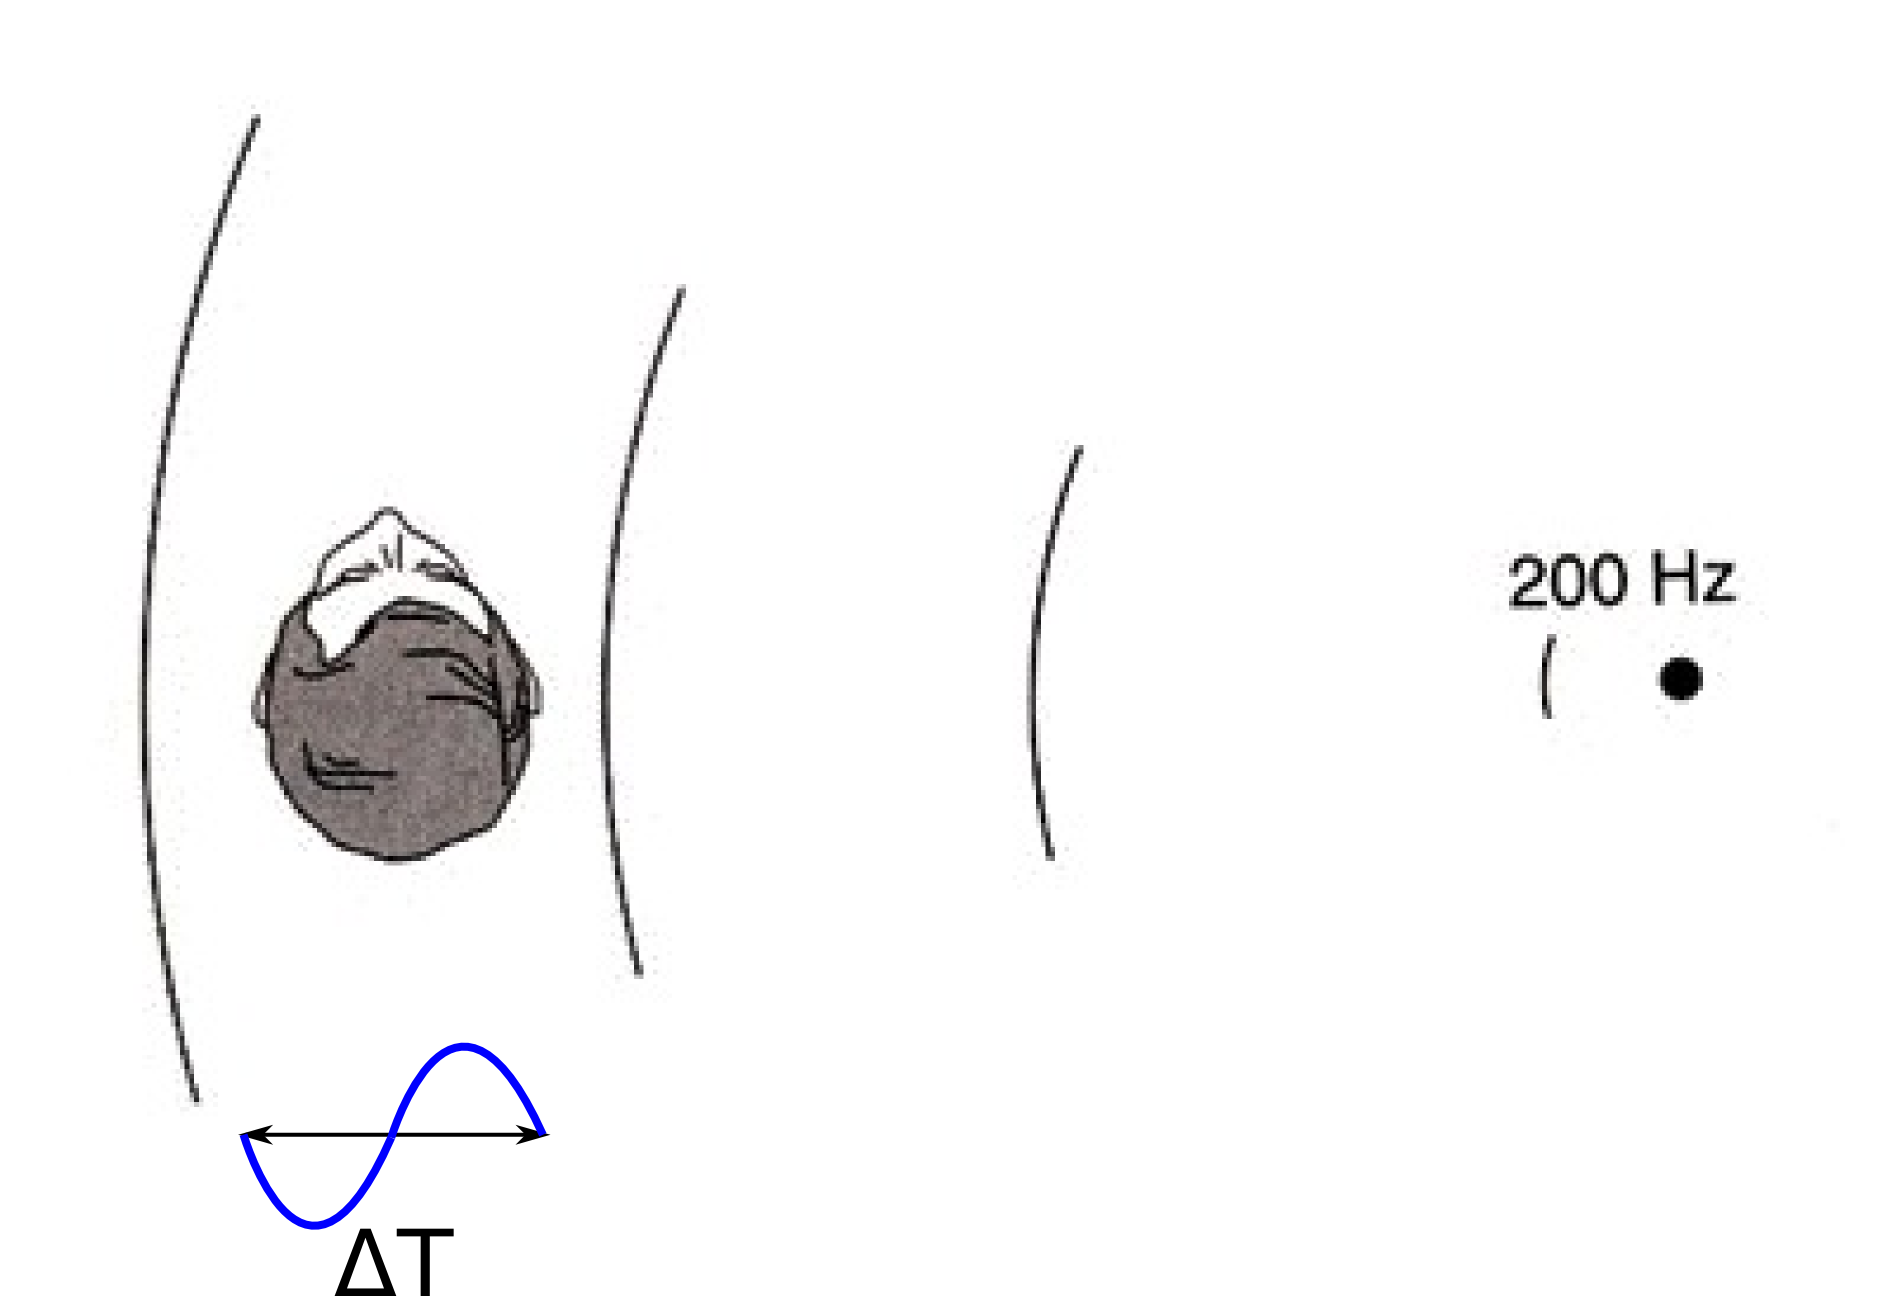
\includegraphics[width = 4.5 cm]{Diagrams/Presentation/HumanITD.png}\\
    \end{column}}
     
   \onslide<1->{\begin{column}{0.5\textwidth}
    \centering
    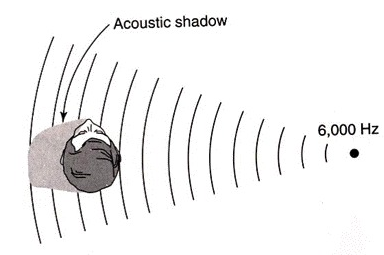
\includegraphics[width = 4.5 cm]{Diagrams/Presentation/HumanILD.png}\\
    \end{column}}
    
  \end{columns}
  
 \begin{exampleblock}
  \onslide<1->{\begin{columns}
 
    \begin{column}{0.5\textwidth}
    \centering
    \underline{\textbf{Interaural Time Difference}}

    \end{column}
     
    \begin{column}{0.5\textwidth}
    \centering
    \underline{\textbf{Interaural Level Difference}}
    \end{column}
    
  \end{columns}
  
    \begin{columns}
 
    \begin{column}{0.5\textwidth}
    %\centering
    \small
     \begin{itemize}
%      \item[]
    \item Phase difference between the (pressure) inputs to the ears.
    \item \textbf{\textcolor{blue}{I}}TD
    \item Used when $\lambda\gg$head size.
     %\item[] Effectively independent eardrum vibrations.
     \end{itemize}
    \end{column}
     
    \begin{column}{0.5\textwidth}
    %\centering
    \small
     \begin{itemize}
          \item Amplitude difference between the inputs.
          \item \textbf{\textcolor{blue}{I}}LD
          \item Used when $\lambda\sim$head size.
     %\item[] Eardrums vibrations influence eachother.
     \end{itemize}
    \end{column}
    
  \end{columns}}
  \end{exampleblock}  
%   \vfill
%   \begin{exampleblock}{}
%   \onslide<2->{\begin{columns}
%  
%     \begin{column}{0.5\textwidth}
%     \centering
%     \underline{\textbf{Internal Time Difference}}
% 
%     \end{column}
%      
%     \begin{column}{0.5\textwidth}
%     \centering
%     \underline{\textbf{Internal Level Difference}}
%     \end{column}
%     
%   \end{columns}
%   
%     \begin{columns}
%  
%     \begin{column}{0.5\textwidth}
%     %\centering
%     \small
%      \begin{itemize}
% %      \item[]
%     \item[] Phase difference between the eardrum \textbf{vibrations}.
%     \item iTD
%      %\item[] Effectively independent eardrum vibrations.
%      \end{itemize}
%     \end{column}
%      
%     \begin{column}{0.5\textwidth}
%     %\centering
%     \small
%      \begin{itemize}
%           \item[] Amplitude difference between the \textbf{vibrations}.
%           \item iLD
%      %\item[] Eardrums vibrations influence eachother.
%      \end{itemize}
%     \end{column}
%     
%   \end{columns}}
%   \end{exampleblock}
\end{frame}

\begin{frame}[t]
 \frametitle{Localization - Coupled Ears}
     \onslide<1>{\begin{exampleblock}{Problems}
% \begin{columns}
%  
%     \begin{column}{0.5\textwidth}
%     %\centering
%     \underline{\textbf{Issues}}
% 
%     \end{column}
%      
%     \begin{column}{0.5\textwidth}
%     %\centering
%     \underline{\textbf{Result}}
%     \end{column}
%     
%   \end{columns}
  
    \begin{columns}
 
     \begin{column}{0.5\textwidth}
    \centering
    \small
     \begin{itemize}
          \item Small heads.
          \item Lower ``processing power''.
     %\item[] Eardrums vibrations influence eachother.
     \end{itemize}
    \end{column}
    
    \begin{column}{0.5\textwidth}
    \centering
    \small
     \begin{itemize}
%      \item[]
    \item ITD$\neq$0, ``small''.
    \item ILD$\approx$0.
     %\item[] Effectively independent eardrum vibrations.
     \end{itemize}
    \end{column}
     
  \end{columns}
  \end{exampleblock}} 
  
  \vfill
  \onslide<2>{\begin{exampleblock}{}
\begin{columns}
 
    \begin{column}{0.5\textwidth}
    \centering
    \underline{\textbf{\textcolor{blue}{Internal} Time Difference}}

    \end{column}
     
    \begin{column}{0.5\textwidth}
    \centering
    \underline{\textbf{\textcolor{blue}{Internal} Level Difference}}
    \end{column}
    
  \end{columns}
  
    \begin{columns}
 
    \begin{column}{0.5\textwidth}
    %\centering
    \small
     \begin{itemize}
%      \item[]
    \item[] Phase difference between \textbf{eardrums}.
    \item \textbf{\textcolor{blue}{i}}TD
    \item \textbf{\textcolor{blue}{i}}TD$>$ITD.
     %\item[] Effectively independent eardrum vibrations.
     \end{itemize}
    \end{column}
     
    \begin{column}{0.5\textwidth}
    %\centering
    \small
     \begin{itemize}
          \item[] Amplitude difference between the \textbf{eardrums}.
          \item \textbf{\textcolor{blue}{i}}LD
          \item \textbf{\textcolor{blue}{i}}LD$>$0.
     %\item[] Eardrums vibrations influence eachother.
     \end{itemize}
    \end{column}
    
  \end{columns}
  \end{exampleblock}}
\end{frame}
  
% \begin{frame}[t]
%  \frametitle{Localization - Coupled Ears}
%   \begin{exampleblock}{}
% \begin{columns}
%  
%     \begin{column}{0.5\textwidth}
%     \centering
%     \underline{\textbf{\textcolor{blue}{Internal} Time Difference}}
% 
%     \end{column}
%      
%     \begin{column}{0.5\textwidth}
%     \centering
%     \underline{\textbf{\textcolor{blue}{Internal} Level Difference}}
%     \end{column}
%     
%   \end{columns}
%   
%     \begin{columns}
%  
%     \begin{column}{0.5\textwidth}
%     %\centering
%     \small
%      \begin{itemize}
% %      \item[]
%     \item[] Phase difference between the eardrum \textbf{vibrations}.
%     \item \textbf{\textcolor{blue}{i}}TD
%      %\item[] Effectively independent eardrum vibrations.
%      \end{itemize}
%     \end{column}
%      
%     \begin{column}{0.5\textwidth}
%     %\centering
%     \small
%      \begin{itemize}
%           \item[] Amplitude difference between the \textbf{vibrations}.
%           \item \textbf{\textcolor{blue}{i}}LD
%      %\item[] Eardrums vibrations influence eachother.
%      \end{itemize}
%     \end{column}
%     
%   \end{columns}
%   \end{exampleblock}  
%   \vfill
%   
%     \onslide<2->{\begin{exampleblock}{Coupled Ears}
% \begin{columns}
%  
%     \begin{column}{0.5\textwidth}
%     \centering
%     \underline{\textbf{Input}}
% 
%     \end{column}
%      
%     \begin{column}{0.5\textwidth}
%     \centering
%     \underline{\textbf{Response}}
%     \end{column}
%     
%   \end{columns}
%   
%     \begin{columns}
%  
%     \begin{column}{0.5\textwidth}
%     \centering
%     \small
%      \begin{itemize}
% %      \item[]
%     \item ITD$\neq$0, ``small''.
%     \item ILD$\approx$0.
%      %\item[] Effectively independent eardrum vibrations.
%      \end{itemize}
%     \end{column}
%      
%     \begin{column}{0.5\textwidth}
%     \centering
%     \small
%      \begin{itemize}
%           \item \textbf{\textcolor{blue}{i}}TD$>$ITD.
%           \item \textbf{\textcolor{blue}{i}}LD$>$0.
%      %\item[] Eardrums vibrations influence eachother.
%      \end{itemize}
%     \end{column}
%     
%   \end{columns}
%   \end{exampleblock}} 
% \end{frame}
%   
% \begin{frame}[t]
%  \begin{exampleblock}{Advantages of Coupled Ears}
%  \begin{itemize}
%   \item Low frequencies result in reduced degradation of hearing cues in dense enviroments.
%  \end{itemize}  
%  \end{exampleblock}
% 
% \end{frame}

\section{The Model}

\begin{frame}[t]
 \frametitle{ICE Model}

\begin{exampleblock}{\textbf{\textcolor{blue}{I}}nternally \textbf{\textcolor{blue}{C}}oupled \textbf{\textcolor{blue}{E}}ars}
 Aim:
 \begin{itemize}
  \item Accurately reproduce the direction and frequency dependence.
  \item[]
  \item Analytically tractable.
 \end{itemize}
\end{exampleblock} 
 \onslide<2->{

 \vfill
 \begin{variableblock}{}{bg= blue!5,fg=black}{bg= blue!5,fg=blue!75}
 Solution:
 \begin{itemize}
%   \item An extension of the model first presented by Vossen et al (2010).
%   \item[]
  \item Circular eardrums. 
  \item[]
  \item Cylindrical mouth cavity.
 \end{itemize}

\end{variableblock}}

\end{frame}

\subsection{Mouth Cavity}
\begin{frame}[t]
\frametitle{Mouth Cavity}
% \begin{figure}[htl]
% \flushleft
% 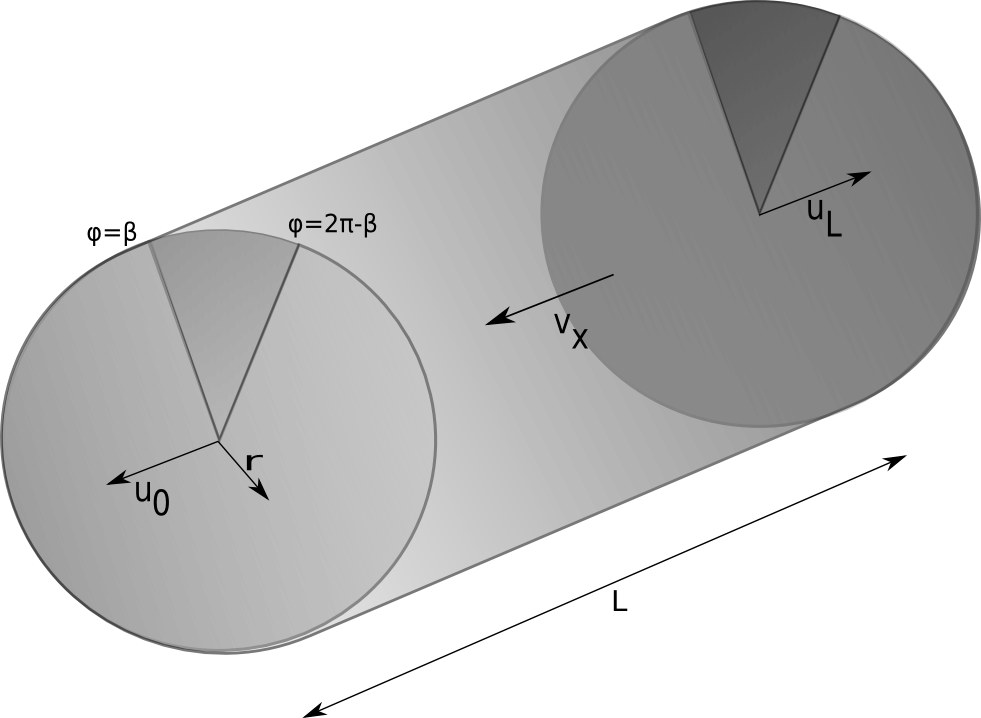
\includegraphics[width=.36\textwidth]{Diagrams/oldCylinder.png}
% %\caption{Previous Cylindrical Cavity}
% \end{figure}
% \begin{figure}[htr]
% 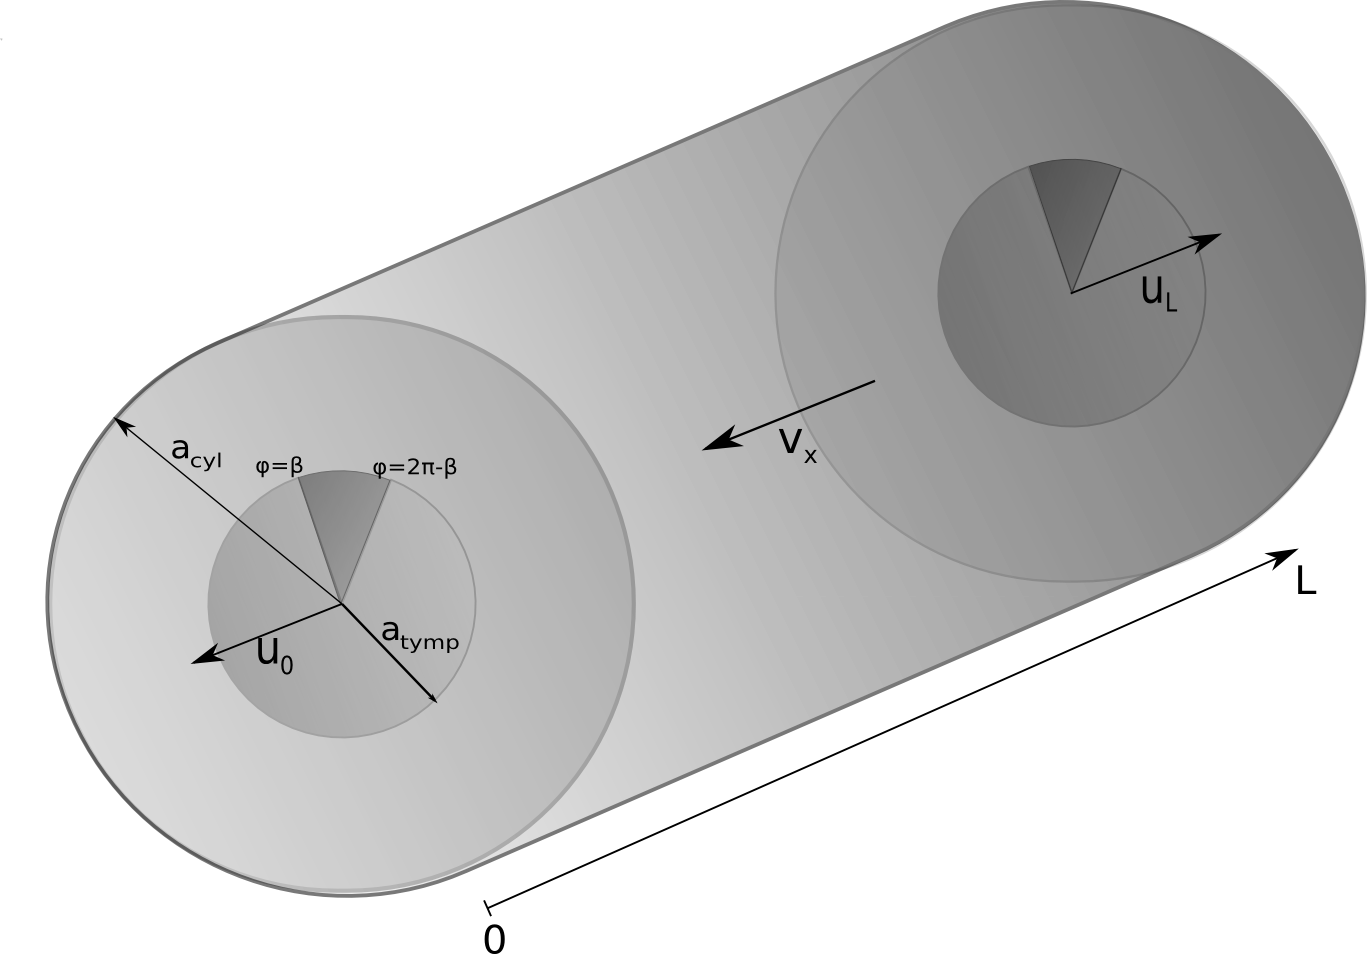
\includegraphics[width=.38\textwidth]{Diagrams/newCylinder.png}
% \caption{Mouth Cavity Model}
% \end{figure}
\begin{columns}

 \begin{column}{0.5\textwidth}
   \onslide<1->{
   \footnotesize
    \underline{\textbf{Previous Model}}$^a$\\
    \centering
    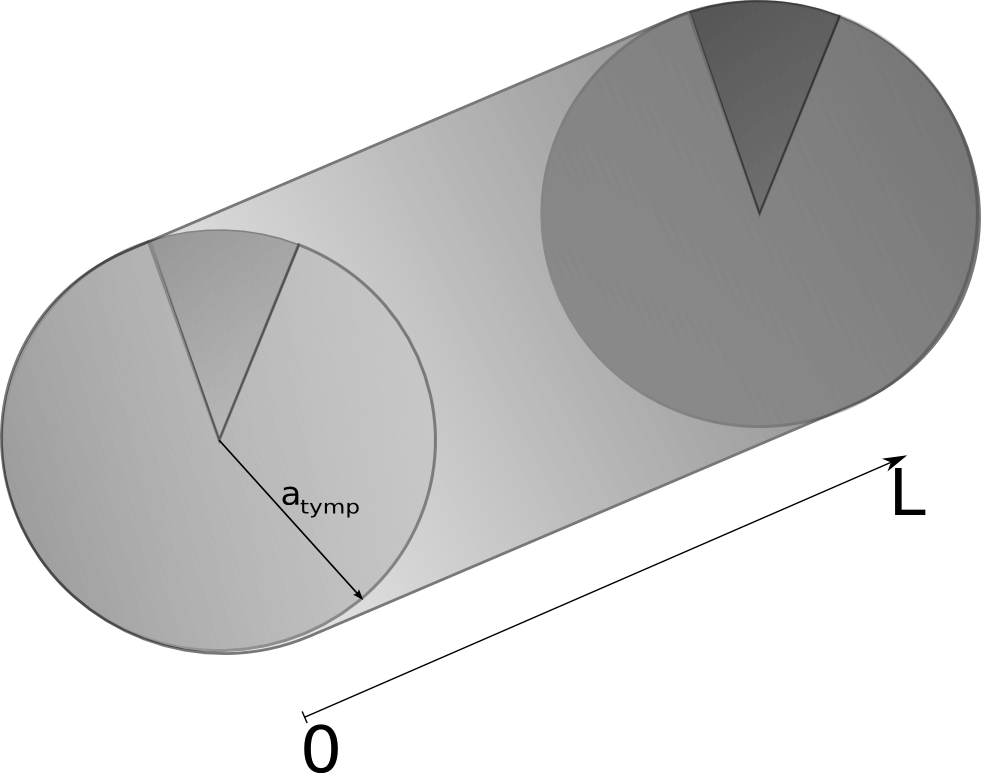
\includegraphics[width = 4 cm]{Diagrams/Presentation/oldCylinder.png}\\
    \small
    \begin{exampleblock}{ }
    \begin{itemize}
     \item[] $a_{\mathrm{tymp}}$ fixed.
     \item[] $V_{\mathrm{cyl}}=\pi a^2_{\mathrm{tymp}}L$
    \end{itemize}
    \end{exampleblock}
    
    \flushleft
    $^a$\footnotesize{Vossen et al (2010)}}

    \end{column}
    
 \begin{column}{0.5\textwidth}
    \onslide<2->{
        \footnotesize
    \underline{\textbf{Our Model}}\\
    \centering
   \includegraphics<2>[width = 4 cm]{Diagrams/Presentation/newCylinder.png}
   
    \small
    \begin{exampleblock}{ }
    \begin{itemize}
     \item[] $a_{\mathrm{tymp}},\ V_{\mathrm{cyl}}$ fixed. 
     \item[] $a_{\mathrm{cyl}}=\sqrt{V_{\mathrm{cyl}}/\pi L}$
    \end{itemize}
    \end{exampleblock}}
    \end{column}
    
    \end{columns}
\end{frame}


\subsubsection{Cavity Pressure}
\begin{frame}[t]
\frametitle{Cavity Pressure - $p(x,r,\phi;t)$}
\begin{exampleblock}{3D Wave Equation}
\begin{equation*}
% \begin{split}
 \frac{1}{c^2}\partial^2_t p=\frac{1}{r}\frac{\partial}{\partial r}\left(r\frac{\partial p}{\partial r}\right)+\frac{1}{r^2}\frac{\partial^2 p}{\partial \phi^2}
 +\frac{\partial p}{\partial x^2}
%  \end{split}
\end{equation*}

\textcolor{blue}{Flow Velocity:}
\begin{equation*}
\dot{\vec{v}}(x,r,\phi;t)=\frac{1}{\rho}\nabla p
 \end{equation*}
\end{exampleblock}

\vfill
\begin{variableblock}{Separation Ansatz}{bg= blue!5,fg=black}{bg= blue!5,fg=blue!75}
\begin{equation*}
 p(x,r,\phi,t)=f(x)g(r)h(\phi)e^{j\omega t}
 \end{equation*}
\end{variableblock}

% Subject to the no-penetration boundary condition at all solid boundaries.

\end{frame}

% \begin{frame}[t]
% \frametitle{Eardrum}
% %  \begin{figure}[ht!]
% %   \centering
% %   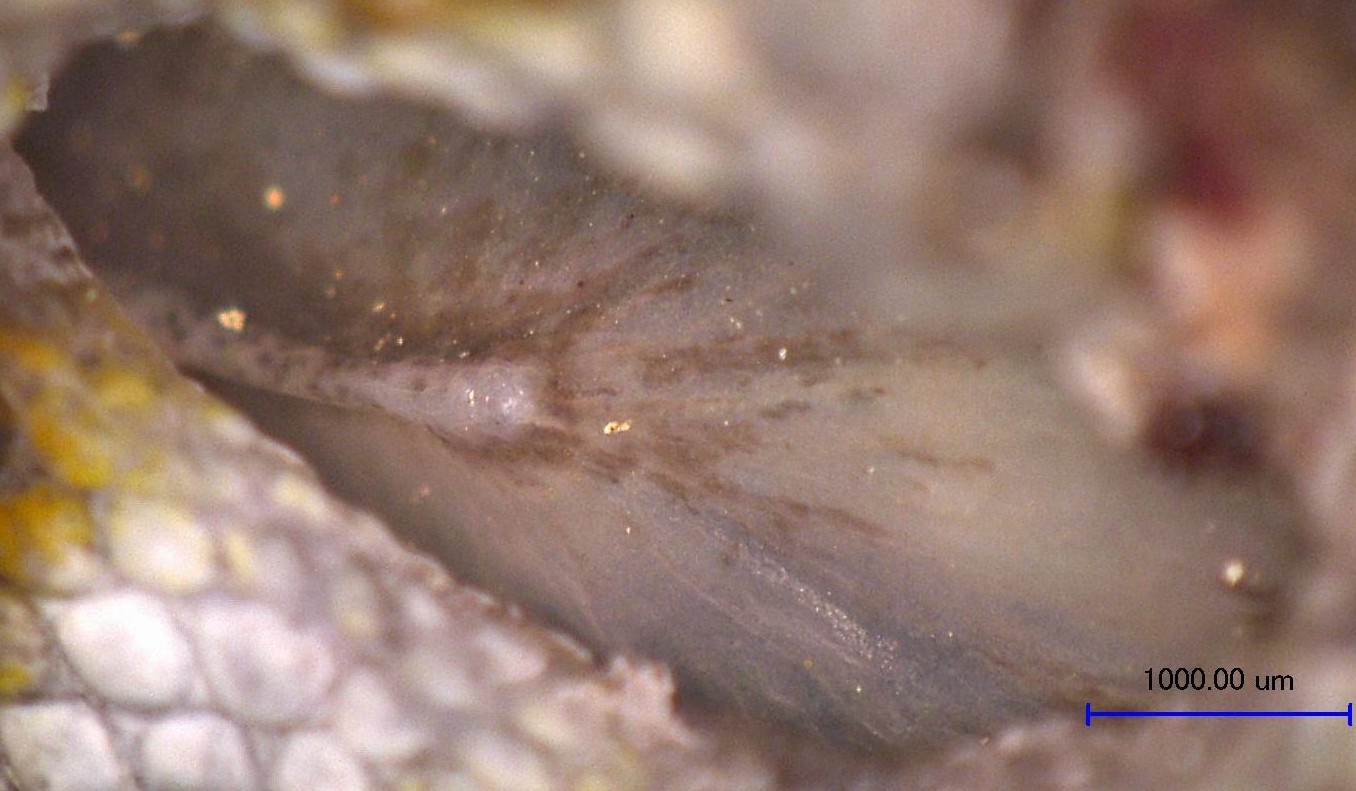
\includegraphics[width=.34\textwidth]{Diagrams/geckoextracolumella2.jpg}
% % \end{figure}
% \begin{figure}[htb!]
% \makebox[\linewidth]{
% 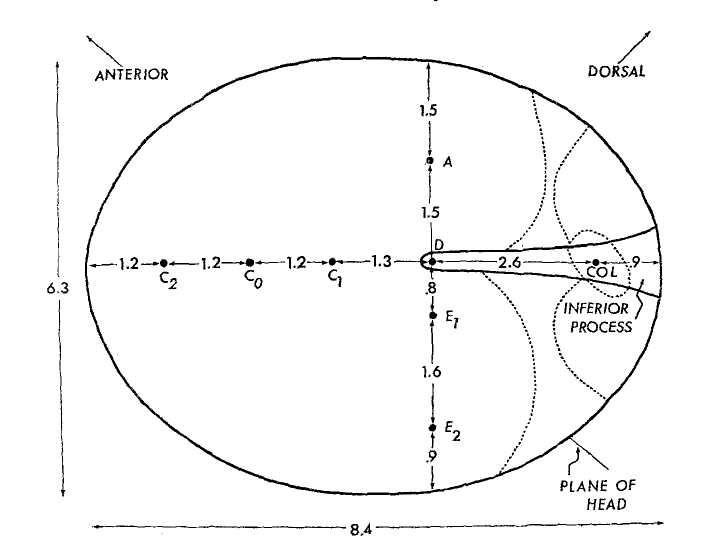
\includegraphics[width=.37\textwidth]{Diagrams/geckoear.png}
% \hfill
% 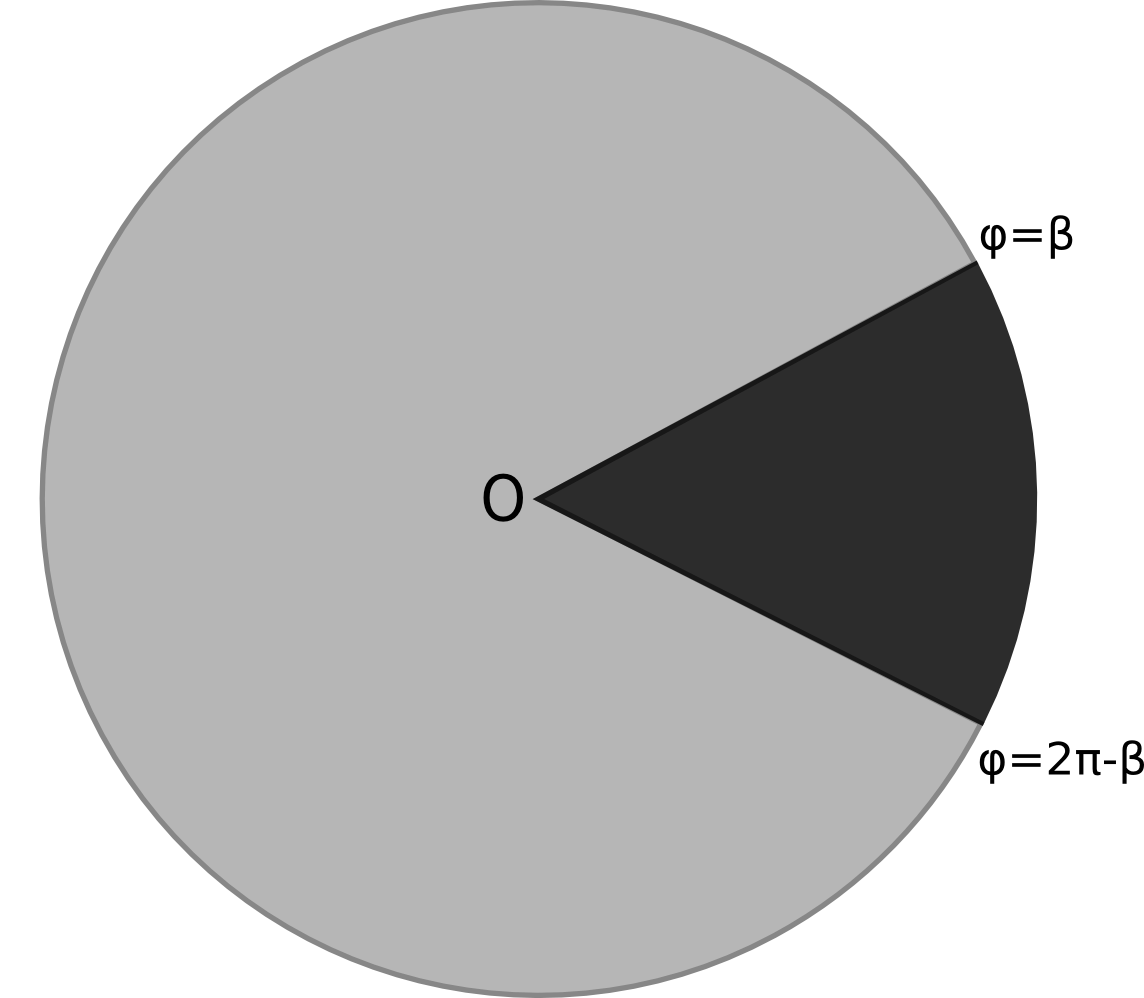
\includegraphics[width=.3\textwidth]{Diagrams/tympanummodel.png}}
% 
% \end{figure}
% 
% \end{frame}

\begin{frame}[t]
\frametitle{Separated Equations}
\onslide<1->{\begin{exampleblock}{$x$- and $\phi$- directions}
\begin{columns}
\begin{column}{.5\textwidth}
 \begin{align*}
 f(x)=Ae^{j\zeta x}+Be^{-j\zeta x}\\
 h(\phi)=Ce^{jq\phi}+De^{-jq\phi}
 \end{align*}
\end{column}
 
 \begin{column}{.5\textwidth}
 \begin{align*}
  &h(\phi)\xrightarrow{cont.,smooth}\cos q\phi\\
  &q=0,1,2,3,\ldots
  \end{align*}
 \end{column}

\end{columns}

\end{exampleblock}}

\onslide<2->{\begin{exampleblock}{$r$-direction, Bessel functions}
%  \begin{equation*}
%  \begin{split}
%   \frac{1}{r}\frac{\partial}{\partial r}\left(r\frac{\partial g(r)}{\partial r}\right)+\left[\nu^2-\frac{q^2}{r^2}\right]g(r)=0
%   &\longrightarrow g(r) = J_q(\nu r)\\
%   &\mbox{where, } \nu^2=k^2-\zeta^2
%   \end{split}
%  \end{equation*}
\begin{columns}
\begin{column}{.5\textwidth}
 \begin{equation*}
 \begin{split}
  &g(r) = J_q(\nu r)\\
  &\\
  &\nu^2=k^2-\zeta^2
  \end{split}
 \end{equation*}
 \end{column}
\begin{column}{.5\textwidth}
 \includegraphics<2>[width=4cm]{Diagrams/Presentation/pressurebessel.png}
\end{column}
  
\end{columns}

\end{exampleblock}}

\end{frame}


\begin{frame}[t]
 \frametitle{Boundary Conditions - $r$}
 
 \onslide<1->{\begin{exampleblock}{Impenetrable boundary at $r=a_{\mathrm{cyl}}$}
 \begin{columns}
 \begin{column}{.65\textwidth}
\begin{align*}
&\mathbf{n_r}.\left.\vec{v}\right|_{r=a_{\mathrm{cyl}}}\equiv\left.\frac{\partial g}{\partial r}\right|_{r=a_{\mathrm{cyl}}}=0\\
&\\
&\Rightarrow g(r)=J_q(\nu_{\mathrm{qs}}r/a_{\mathrm{cyl}})
\end{align*}
\end{column}

\begin{column}{.35\textwidth}
\centering
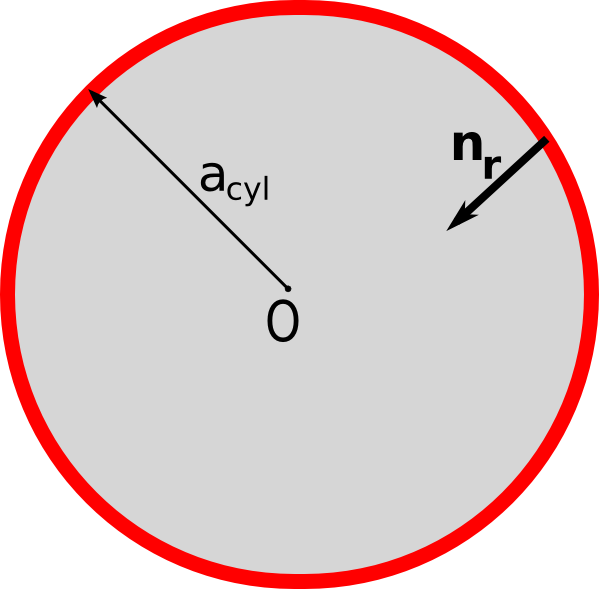
\includegraphics[width = 2.5cm]{Diagrams/Presentation/BoundaryConditions/cylinderradial.png}
\end{column}
\end{columns}
\end{exampleblock}}

\onslide<2->{\begin{variableblock}{Bessel Prime Zeros}{bg= blue!5,fg=black}{bg= blue!5,fg=blue!75}
 \begin{columns}
 \begin{column}{.4\textwidth}
\begin{itemize}
 \centering
 \item[] $\nu_{\mathrm{qs}}$ - extrema of $J_q$.
 \item[] $\nu_{\mathrm{00}}$=0.
 \end{itemize}
 \end{column}
 \begin{column}{.6\textwidth}
  \centering
\includegraphics<2>[width = 3.5cm]{Diagrams/Presentation/BoundaryConditions/besselprimezeros.png}
 \end{column}
\end{columns}
\end{variableblock}}


\end{frame}

% \begin{frame}[t]
%  \frametitle{Boundary Conditions - $\phi$}
%  \begin{exampleblock}{Smoothness and Continuity in $\phi$.}
%  \begin{columns}
%  \begin{column}{.65\textwidth}
%   \begin{align*}
%    &h(0)=h(2\pi)\nonumber\\
%    &h^\prime(0)=h^\prime(2\pi)\nonumber\\
%    &\mbox{}\nonumber\\
%    \Rightarrow &h(\phi)=\cos q\phi\\
%    &q=0,1,2,\ldots\nonumber
%   \end{align*}
%   \end{column}
%   \begin{column}{.35\textwidth}
%    \centering
% 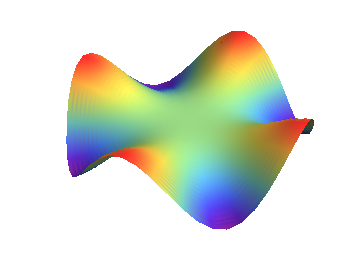
\includegraphics[width = 3.0cm]{Diagrams/Presentation/BoundaryConditions/cylinderphi.png}
%   \end{column}
% 
%   \end{columns}
%  \end{exampleblock}
% \end{frame}
% \left.\frac{\partial J_q(\nu_{\mathrm{qs}}r)}{\partial r}\right|_{r=a_{\mathrm{cyl}}}=0

\begin{frame}[t]
\frametitle{General Solution}
\begin{exampleblock}{Pressure Modes}
%   \begin{equation*}
%    &p_{\mathrm{qs}}(r,\phi)=\cos q\phi J_q(\nu_{\mathrm{qs}}r/a_{\mathrm{cyl}})\nonumber\\
%    &\nonumber\\
%    &p(x,r,\phi,t)=\displaystyle\sum^{\infty}_{q=0,s=0}\left[A_{\mathrm{qs}}e^{j\zeta_{\mathrm{qs}}x}+B_{\mathrm{qs}}e^{-j\zeta_{\mathrm{qs}}x}\right]p_{\mathrm{qs}}(r,\phi)e^{j\omega t}\\
%    %&\zeta_{\mathrm{qs}}=\sqrt{k^2-\nu^2_{\mathrm{qs}}/a^2_{\mathrm{cyl}}}\nonumber
%   \end{equation*}
\begin{columns}
\begin{column}{.4\textwidth}
%\begin{center}
 \begin{tabular}{cc}
 %\centering
  \includegraphics<1->[width = 2.2 cm]{Diagrams/Presentation/BoundaryConditions/presmode00.png} & \includegraphics<1->[width = 2.2 cm]{Diagrams/Presentation/BoundaryConditions/presmode11.png} \\
 \includegraphics<1->[width = 2.2 cm]{Diagrams/Presentation/BoundaryConditions/presmode21.png} &  \includegraphics<1->[width = 2.2 cm]{Diagrams/Presentation/BoundaryConditions/presmode02.png}
\end{tabular}
%\end{center}
\end{column}

 \begin{column}{.6\textwidth}

 \begin{itemize}
    \item<1>[] $p_{\mathrm{qs}}(r,\phi)=\cos q\phi J_q(\nu_{\mathrm{qs}}r/a_{\mathrm{cyl}})$
   \item[]
   %\vspace{4pt}
   
   \item<1>[] $f_{\mathrm{qs}}(x)=A_{\mathrm{qs}}e^{j\zeta_{\mathrm{qs}}x}+B_{\mathrm{qs}}e^{-j\zeta_{\mathrm{qs}}x}$
   \item[]
\item<2>[] $\int dS p_{\mathrm{qs}}\neq0$ iff $q=0,\ s=0$
\item[]
\item<2>[] 	$\int dS p_{\mathrm{qs}}p_{\mathrm{mn}}=\delta_{qm}\delta_{sn}$
\end{itemize}
   \end{column}

\end{columns}
   %&\zeta_{\mathrm{qs}}=\sqrt{k^2-\nu^2_{\mathrm{qs}}/a^2_{\mathrm{cyl}}}\nonumber

% \begin{tabular}{cc}
%   \includegraphics<1>[width = 2.2 cm]{Diagrams/Presentation/BoundaryConditions/presmode00.png} & \includegraphics<1>[width = 2.2 cm]{Diagrams/Presentation/BoundaryConditions/presmode11.png} \\
%  \includegraphics<1>[width = 2.2 cm]{Diagrams/Presentation/BoundaryConditions/presmode21.png} &  \includegraphics<1>[width = 2.2 cm]{Diagrams/Presentation/BoundaryConditions/presmode02.png}
% \end{tabular}

%$p(x,r,\phi,t)=\displaystyle\sum^{\infty}_{q=0,s=0}f_{\mathrm{qs}}(x)p_{\mathrm{qs}}(r,\phi)e^{j\omega t}$
% $p(x,r,\phi,t)=\displaystyle\sum^{\infty}_{q=0,s=0}\left[A_{\mathrm{qs}}e^{j\zeta_{\mathrm{qs}}x}+B_{\mathrm{qs}}e^{-j\zeta_{\mathrm{qs}}x}\right]p_{\mathrm{qs}}(r,\phi)e^{j\omega t}$

 \end{exampleblock}
% \onslide<2>{\begin{variableblock}{}{bg= blue!5,fg=black}{bg= blue!5,fg=blue!75}
%  \begin{equation*}
%    \zeta_{\mathrm{qs}}=\sqrt{k^2-\nu^2_{\mathrm{qs}}/a^2_{\mathrm{cyl}}}\nonumber
%  \end{equation*}
% \end{variableblock}
%}
\end{frame}

\subsection{Eardrum}
\subsubsection{Model}
\begin{frame}[t]
\frametitle{Eardrum}
\begin{columns}
    \begin{column}{0.5\textwidth}
      \centering
      \small
      Sketch of a Tokay eardrum as seen from the outside (G.A. Manley, 1972).\\
      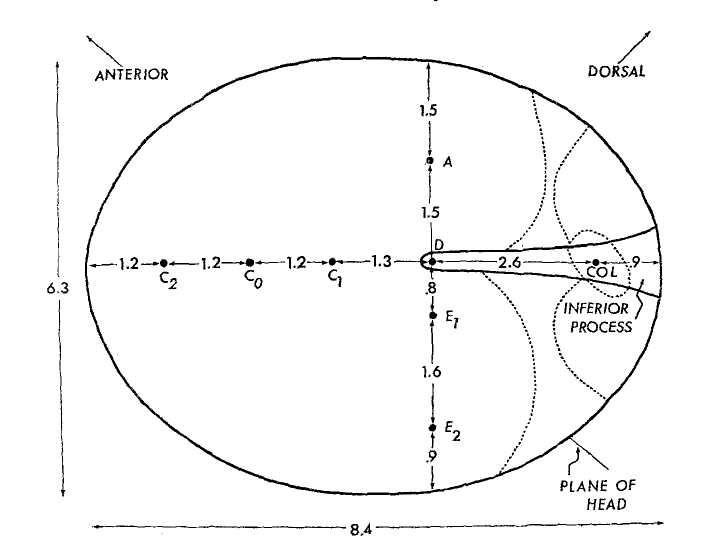
\includegraphics[width = 3.7 cm]{Diagrams/geckoear.png}\\
      \small
     COL - approximate position opposite the extracolumella insertion.
    \end{column}

    \begin{column}{0.5\textwidth}
      \centering
      \small
      The ICE Eardrum.\\
      \textbf{}\\
      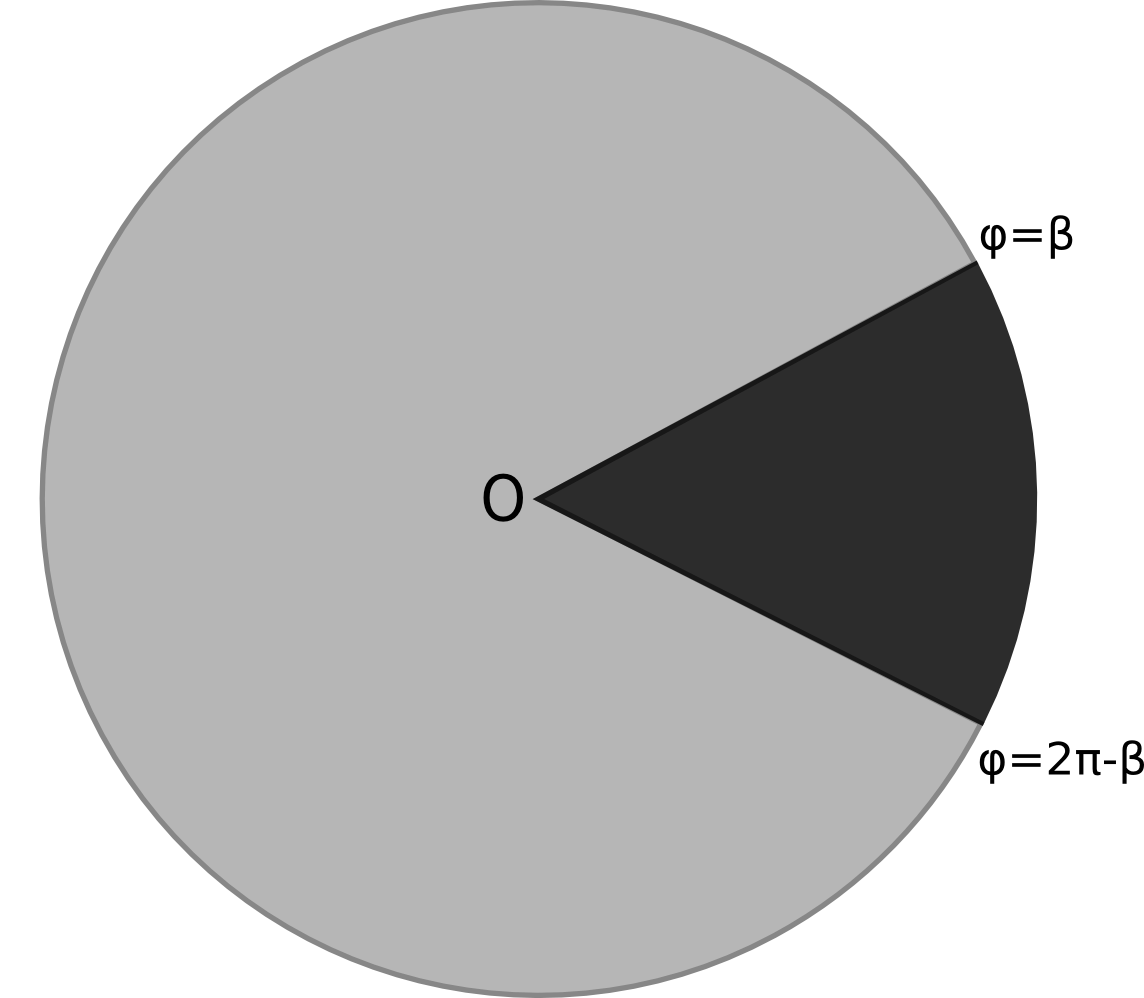
\includegraphics[width = 3.2 cm]{Diagrams/tympanummodel.png}\\
%       \textbf{}\\
%       Extracolumella (dark region) is rigid and stationary.\\
%       \textbf{}\\
%       The membrane material is assumed to be linear elastic.
\small
\begin{itemize}
      \item[] Extracolumella (dark) - \textcolor{red}{rigid}, \textcolor{red}{stationary}.
      \item[] Membrane - \textcolor{blue}{linear elastic}.
      \item[] Clamped at boundaries ($r=a_{\mathrm{tymp}}$, $\phi=\beta,\ 2\pi-\beta$)
\end{itemize}

    \end{column}
  \end{columns}
  
\end{frame}

\subsubsection{Membrane Vibrations}

\begin{frame}[t]
 \frametitle{Membrane Vibrations}
\onslide<1>{\begin{exampleblock}{Membrane Displacement - $u(r,\phi;t)$}

\begin{equation*}
%\begin{split}
 -\partial^2_tu-2\textcolor{red}{\alpha}\partial_t u+\textcolor{blue}{c}^2_{\textcolor{blue}{m}} \Delta_{(2)}u=\frac{1}{\textcolor{red}{\rho_m} \textcolor{blue}{d}}\Psi(r,\phi;t)
 %\end{split}
\end{equation*}
 \end{exampleblock}}
\vfill
\begin{variableblock}{Membrane Parameters}{bg= blue!5,fg=black}{bg= blue!5,fg=blue!75}
\begin{center}
  \begin{tabular}{l l}
    $\textcolor{red}{\alpha}$ - damping coefficient, &  $\textcolor{blue}{c_m}$ - propagation velocity\\
    \hspace{1pt}\\
    $\textcolor{red}{\rho_m}$ - density, & $\textcolor{blue}{d}$ - thickness.
  \end{tabular}
\end{center}
\end{variableblock}
% \begin{columns}
% \begin{column}{\textwidth}
% \begin{variableblock}{Membrane Parameters}{bg= blue!5,fg=black}{bg= blue!5,fg=blue!75}
%   \begin{tabular}{l l}
%     $\textcolor{red}{\alpha}$ - damping coefficient, &  $\textcolor{blue}{c_m}$ - propagation velocity\\
%     \hspace{1pt}\\
%     $\textcolor{red}{\rho_m}$ - density, & $\textcolor{blue}{d}$ - thickness.
%   \end{tabular}
%   \end{variableblock}
% \onslide<1>{\begin{variableblock}{Membrane Parameters}{bg= blue!5,fg=black}{bg= blue!5,fg=blue!75}
%   \begin{tabular}{l}
%     $\textcolor{red}{\alpha}$ - damping coefficient\\
%     \hspace{2pt}\\
%     $\textcolor{blue}{c_m}$ - propagation velocity\\
%     \hspace{2pt}\\
%     $\textcolor{red}{\rho_m}$ - density\\
%     \hspace{2pt}\\
%     $\textcolor{blue}{d}$ - thickness.
%   \end{tabular}
%  \end{variableblock}}
% \end{column}
% \begin{column}{.5\textwidth}
%  \onslide<2>{\begin{variableblock}{Separation Ansatz}{bg= blue!5,fg=black}{bg= blue!5,fg=blue!75}
%  $u(r,\phi;t)=f(r)g(\phi)h(t)\nonumber$
% % Same set of equations as in the pressure case.
% \end{variableblock}}
% \end{column}
% \end{columns}

\end{frame}

\begin{frame}[t]
 \frametitle{Free-Undamped Membrane, $\alpha\rightarrow 0$, $\Psi\rightarrow 0$}
% \onslide<1->{\begin{exampleblock}{Membrane EOM}
% 
% \begin{equation*}\label{membraneequation1}
% \begin{split}
%  -\partial^2_tu(r,\phi;t)-2\alpha\partial_t u(r,\phi;t)+c^2_m\Delta_{(2)}&u(r,\phi;t)=\\ 
%  & \frac{1}{\rho_m d}\Psi(r,\phi;t)
%  \end{split}
% \end{equation*}
%  \end{exampleblock}}
% 
\onslide<1->{\begin{variableblock}{Separation Ansatz}{bg= blue!5,fg=black}{bg= blue!5,fg=blue!75}
\begin{equation*}\label{mseparationansatz}
 u(r,\phi;t)=f(r)g(\phi)h(t)\nonumber
\end{equation*}
% Same set of equations as in the pressure case.
\end{variableblock}}
% \begin{exampleblock}{Separated Equations}
%  \begin{align*}
%    \frac{d^2 g(\phi)}{d\phi^2}+\kappa^2g(\phi)&=0\\
%    \frac{1}{r}\frac{\partial}{\partial r}\left(r\frac{\partial f(r)}{\partial r}\right)+\left[\mu^2-\frac{\kappa^2}{r^2}\right]f(r)&=0\\
%  \frac{d^2 h(t)}{dt^2}+c^2_m\mu^2h(t)&=0
% \end{align*}
% \end{exampleblock}
\vfill
 \onslide<2->{\textcolor{blue}{Boundary Conditions}
\begin{exampleblock}{$\phi$-direction: $u(r,\beta;t)=u(r,2\pi-\beta,t)=0$}
 \begin{columns}
      \begin{column}{.3\textwidth}
      \centering
      \includegraphics<2->[width = 2.5 cm]{Diagrams/Presentation/BoundaryConditions/bc2.png}
     \end{column}
     
     \begin{column}{.7\textwidth}  
\begin{align*}
  \Rightarrow &g(\phi)=\sin\kappa(\phi-\beta)\nonumber\\
  &\kappa=\frac{m\pi}{2(\pi-\beta)}, m=1,2,\ldots\nonumber
  \end{align*}
     \end{column}

  \end{columns}
 \end{exampleblock}}

\end{frame}

\begin{frame}[t]
 \frametitle{Boundary Conditions contd.}
%  \onslide<1->{\begin{exampleblock}{$\phi$-direction: $u(r,\beta;t)=u(r,2\pi-\beta,t)=0$}
%  \begin{columns}
%       \begin{column}{.3\textwidth}
%       \centering
%       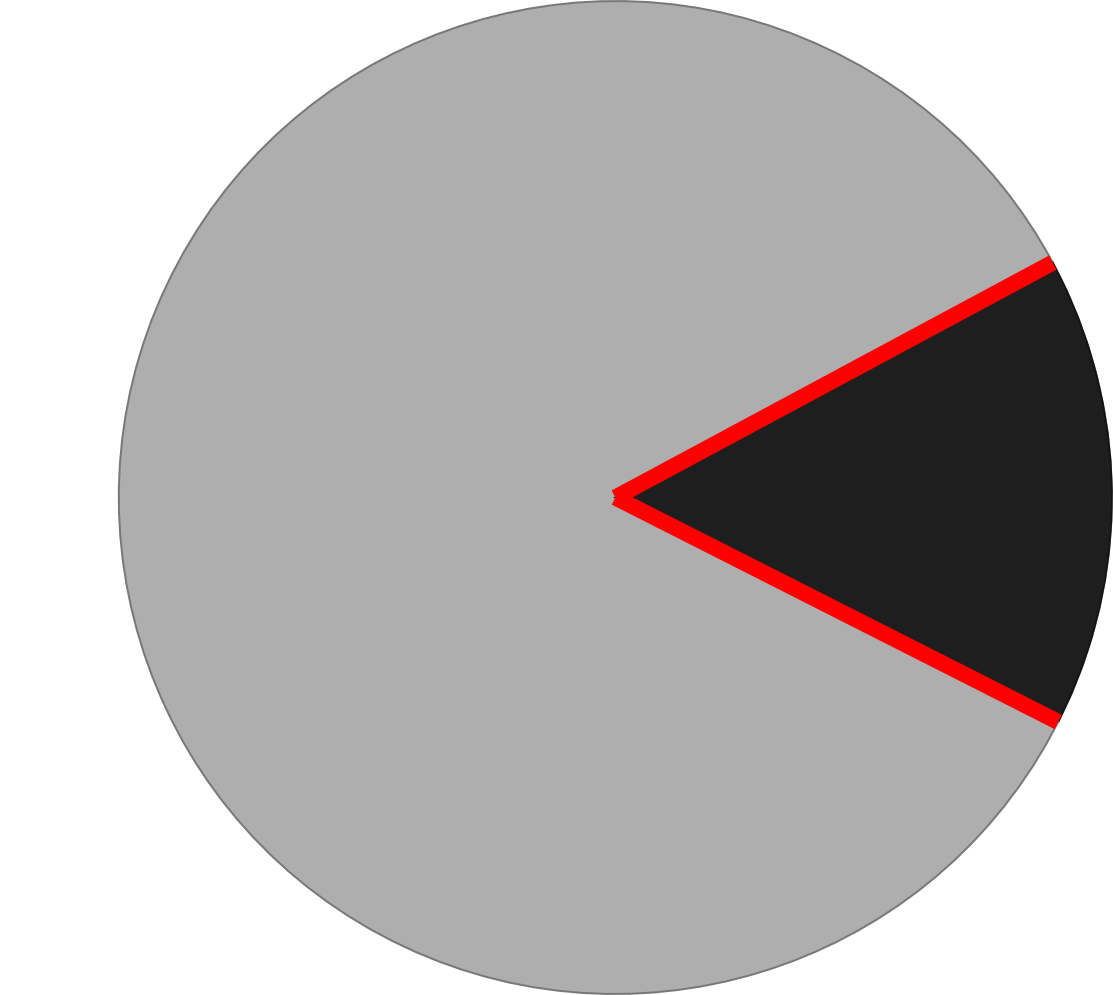
\includegraphics[width = 2.5 cm]{Diagrams/Presentation/BoundaryConditions/bc2.png}
%      \end{column}
%      
%      \begin{column}{.7\textwidth}  
% \begin{align*}
%   \Rightarrow &g(\phi)=\sin\kappa(\phi-\beta)\nonumber\\
%   &\kappa=\frac{m\pi}{2(\pi-\beta)}, m=1,2,\ldots\nonumber
%   \end{align*}
%      \end{column}
% 
%   \end{columns}
%  \end{exampleblock}}
 \begin{exampleblock}{$r$-direction: $u(a_{\mathrm{tymp}},\phi;t)=0$}
 \onslide<1->{\begin{columns}
 \begin{column}{.3\textwidth}
      \centering
      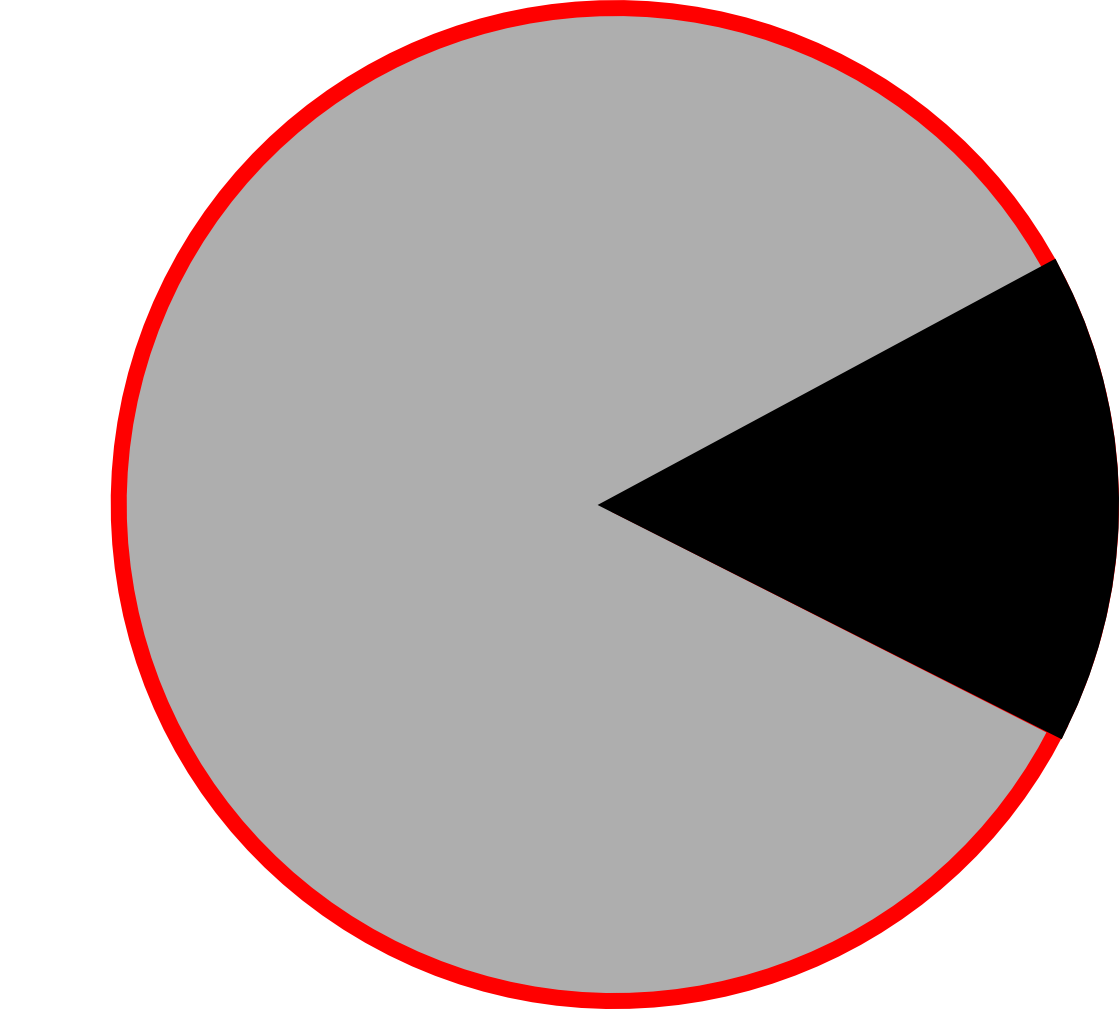
\includegraphics[width = 2.5 cm]{Diagrams/Presentation/BoundaryConditions/bc1.png}
     \end{column}
     \begin{column}{.7\textwidth}  
  \begin{align*}
  \Rightarrow &f(r)=J_\kappa(\mu_{\mathrm{mn}}r/a_{\mathrm{tymp}})\nonumber\\
  &\mu_{\mathrm{mn}} \mbox{:}\ n^{\mathrm{th}} \mbox{ zero of } J_\kappa\nonumber
  \end{align*}
  \end{column}
       
     \end{columns}}
\begin{figure}[h!]
      \centering
      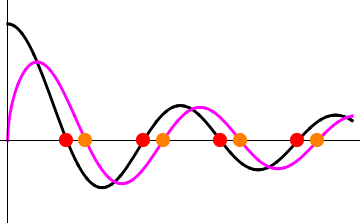
\includegraphics[width = 5.5 cm]{Diagrams/Presentation/BoundaryConditions/besselzeros.png}
 \end{figure}
 \end{exampleblock}

\end{frame}

\begin{frame}[t]
 \frametitle{}
 \onslide<1>{\begin{exampleblock}{Free Membrane Eigenmodes - $u_{\mathrm{mn}}(r,\phi)$}
% \begin{columns}
%  \begin{column}{.2\textwidth}
%  \centering
%   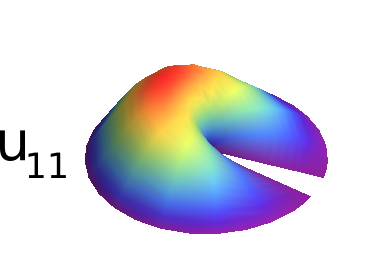
\includegraphics[width = 2.3 cm]{Diagrams/Presentation/BoundaryConditions/membmode1.png}\\
%  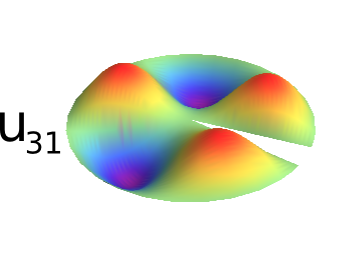
\includegraphics[width = 2.3 cm]{Diagrams/Presentation/BoundaryConditions/membmode3.png}
%  \end{column}
%  \begin{column}{.2\textwidth}
%  \centering
%  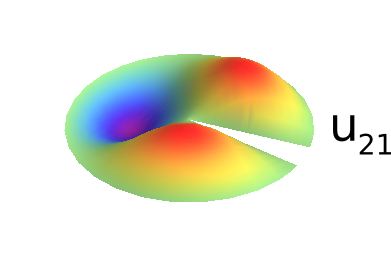
\includegraphics[width = 2.3 cm]{Diagrams/Presentation/BoundaryConditions/membmode2.png} \\
%   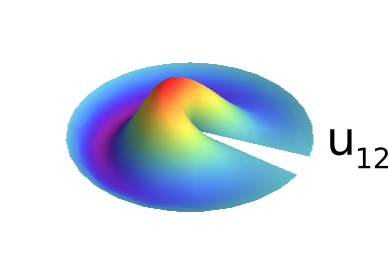
\includegraphics[width = 2.3 cm]{Diagrams/Presentation/BoundaryConditions/membmode4.png}
%  \end{column}
% 
% \end{columns}
%$u_{\mathrm{mn}}(r,\phi)=\sin \kappa(\phi-\beta) J_\kappa(\mu_{\mathrm{mn}} r)$
\begin{columns}
\begin{column}{.6\textwidth}
\begin{center}

%\begin{overlayarea}{\textwidth}{1cm}
\begin{tabular}{cc}
  \includegraphics<1>[width = 2.2 cm]{Diagrams/Presentation/BoundaryConditions/membmode1.png} & \includegraphics<1>[width = 2.2 cm]{Diagrams/Presentation/BoundaryConditions/membmode2.png} \\
 \includegraphics<1>[width = 2.2 cm]{Diagrams/Presentation/BoundaryConditions/membmode3.png} &  \includegraphics<1>[width = 2.2 cm]{Diagrams/Presentation/BoundaryConditions/membmode4.png}
\end{tabular}
%\end{overlayarea}
\end{center}
\end{column}
\begin{column}{.4\textwidth}
\begin{center}
\begin{tabular}{l}
$\omega_{\mathrm{mn}}=c_m\mu_{\mathrm{mn}}$\\
\hspace{1pt} \\
$h(t)=\mathrm{exp}\left(j\omega_{\mathrm{mn}}t\right)$\\
\hspace{1pt} \\
$\int dS u_{\mathrm{kl}}u_{\mathrm{mn}}=\delta_{km}\delta_{ln}$
\end{tabular}
\end{center}
\end{column}
\end{columns}
%                 \begin{equation*}
%   &u_{\mathrm{free}}(r,\phi;t)=\displaystyle\sum^\infty_{m=0,n=1}C_\mathrm{mn}u_{\mathrm{mn}}(r,\phi)e^{j\omega_{\mathrm{mn}} t}\\
%   &\mbox{where, }\omega_{\mathrm{mn}}=c_m\mu_{\mathrm{mn}}\nonumber
%   \end{equation*}
             \end{exampleblock}}
             \vfill
             \onslide<2>{\begin{variableblock}{Damped: $\alpha\neq0$}{bg= blue!5,fg=black}{bg= blue!5,fg=blue!75}
			  \begin{align*}
                          h(t)&=\mathrm{exp}\left(-\alpha t+j\widetilde{\omega}_\mathrm{mn}t\right)\\
                          \mbox{}\\
                          \widetilde{\omega}_\mathrm{mn}&=\sqrt{\omega^2_{\mathrm{mn}}+\alpha^2}
                          \end{align*}
                         \end{variableblock}}

%  \onslide<1->{\begin{exampleblock}{Free eigenmodes}
%   \begin{align*}
%   &u_{\mathrm{mn}}(r,\phi)=\sin \kappa(\phi-\beta) J_\kappa(\mu_{\mathrm{mn}} r)\\
%   &u_{\mathrm{free}}(r,\phi;t)=\displaystyle\sum^\infty_{m=0,n=1}C_\mathrm{mn}u_{\mathrm{mn}}(r,\phi)e^{j\omega_{\mathrm{mn}} t}\\
%   &\mbox{where, }\omega_{\mathrm{mn}}=c_m\mu_{\mathrm{mn}}\nonumber
%   \end{align*}
%  \end{exampleblock}}
% \onslide<2->{\begin{exampleblock}{Damped membrane}
%               \begin{equation*}
%                \widetilde{u}_{\mathrm{free}}(r,\phi;t)=\displaystyle\sum^\infty_{m=0,n=1}\widetilde{C}_{\mathrm{mn}}u_{\mathrm{mn}}(r,\phi)e^{j\omega_{\mathrm{mn}} t-\alpha t}
%               \end{equation*}
%              \end{exampleblock}}
\end{frame}

\begin{frame}[t]
 \frametitle{Forced Vibrations: $\Psi=\mbox{p}e^{j\omega t}$, $\alpha\neq0$}
 \onslide<1->{\begin{exampleblock}{Steady State Solution}
  \begin{equation*}
  u_{\mathrm{ss}}(r,\phi;t)=:\displaystyle\sum^\infty_{m=0,n=1}\textcolor{red}{C_{\mathrm{mn}}}u_{\mathrm{mn}}(r,\phi)e^{j\omega t}
  \end{equation*}
 \end{exampleblock}}
 \vfill
 \onslide<2->{\begin{variableblock}{}{bg= blue!5,fg=black}{bg= blue!5,fg=blue!75}
   Substitute $u_{\mathrm{ss}}$ in Membrane equation.
               \begin{align*}
               &\textcolor{red}{C_{\mathrm{mn}}}=\frac{p\int dS u_{\mathrm{mn}}}{\Omega_{\mathrm{mn}}\int dS u^2_{\mathrm{mn}}}\\
               &\\
                &\Omega_{\mathrm{mn}}=\rho_M d \left[(\omega^2-\omega^2_{\mathrm{mn}})-2j\alpha\omega\right]\nonumber
               \end{align*}

              \end{variableblock}}

\end{frame}
\begin{frame}[t]
\frametitle{Forced Vibrations contd.}
 \onslide<1>{\begin{exampleblock}{Transient Solution}
$\equiv$ free damped membrane
              \begin{equation*}
               u_{\mathrm{t}}(r,\phi;t)=\displaystyle\sum^\infty_{m=0,n=1}\widetilde{C}_{\mathrm{mn}}u_{\mathrm{mn}}(r,\phi)e^{j\widetilde{\omega}_{\mathrm{mn}} t-\alpha t}
               \end{equation*}
%$\widetilde{\omega}_{\mathrm{mn}}=\sqrt{\omega^2_{\mathrm{mn}}+\alpha^2}$\\
\vspace{2pt}

\noindent $u(r,\phi;0)=0 \Rightarrow\ \widetilde{C}_{\mathrm{mn}}=-C_{\mathrm{mn}}$.

\end{exampleblock}}
\vfill
\onslide<2->{\begin{variableblock}{Steady State Approximation}{bg= blue!5,fg=black}{bg= blue!5,fg=blue!75}
\noindent $u_{\mathrm{t}}\rightarrow 0$ exponentially as $t\rightarrow\infty$.

\centering $\textcolor{red}{u\approx u_{\mathrm{ss}}}$
\end{variableblock}}

\end{frame}

\subsection{Acoustic Head Model}
\begin{frame}[t]
 \frametitle{Acoustic Head Model - previous}
 \begin{columns}
     \begin{column}{.5\textwidth}
    \small
    \flushleft
     \onslide<1>{\begin{itemize}
      \item[$\bullet$] \textbf{I} - Ipsilateral, \textbf{C} - Contralateral.
      \item[$\bullet$]  $p_0,\ p_L$ - Sound pressure.
      \item[$\bullet$] $\theta$ - Source direction.
      \item[$\bullet$] Sound source ``far away''.
     \end{itemize}}
     \hspace{2pt}
     
     \begin{itemize}
      \item<2> $|p_0|=|p_L|$.
      \item<2> $\Delta=kL\sin\theta$.
      \item[]
       \item<3>[$\bullet$] $p_0=\mbox{p}\mathrm{ exp}\left(- j\Delta/2\right)$\\ $p_L=\mbox{p}\mathrm{ exp}\left(j\Delta/2\right)$
      %\item[]
      \item<3>[$\bullet$] ILD=0, ITD$\vcentcolon=\frac{1}{\omega}\mbox{Arg}\left(\frac{p^0}{p^L}\right)=$L/c
      \end{itemize}

    \end{column}
    
    
 \begin{column}{0.5\textwidth}
%     \centering
%     \small
%     \underline{\textbf{Head Model}}\\
%     \flushleft
    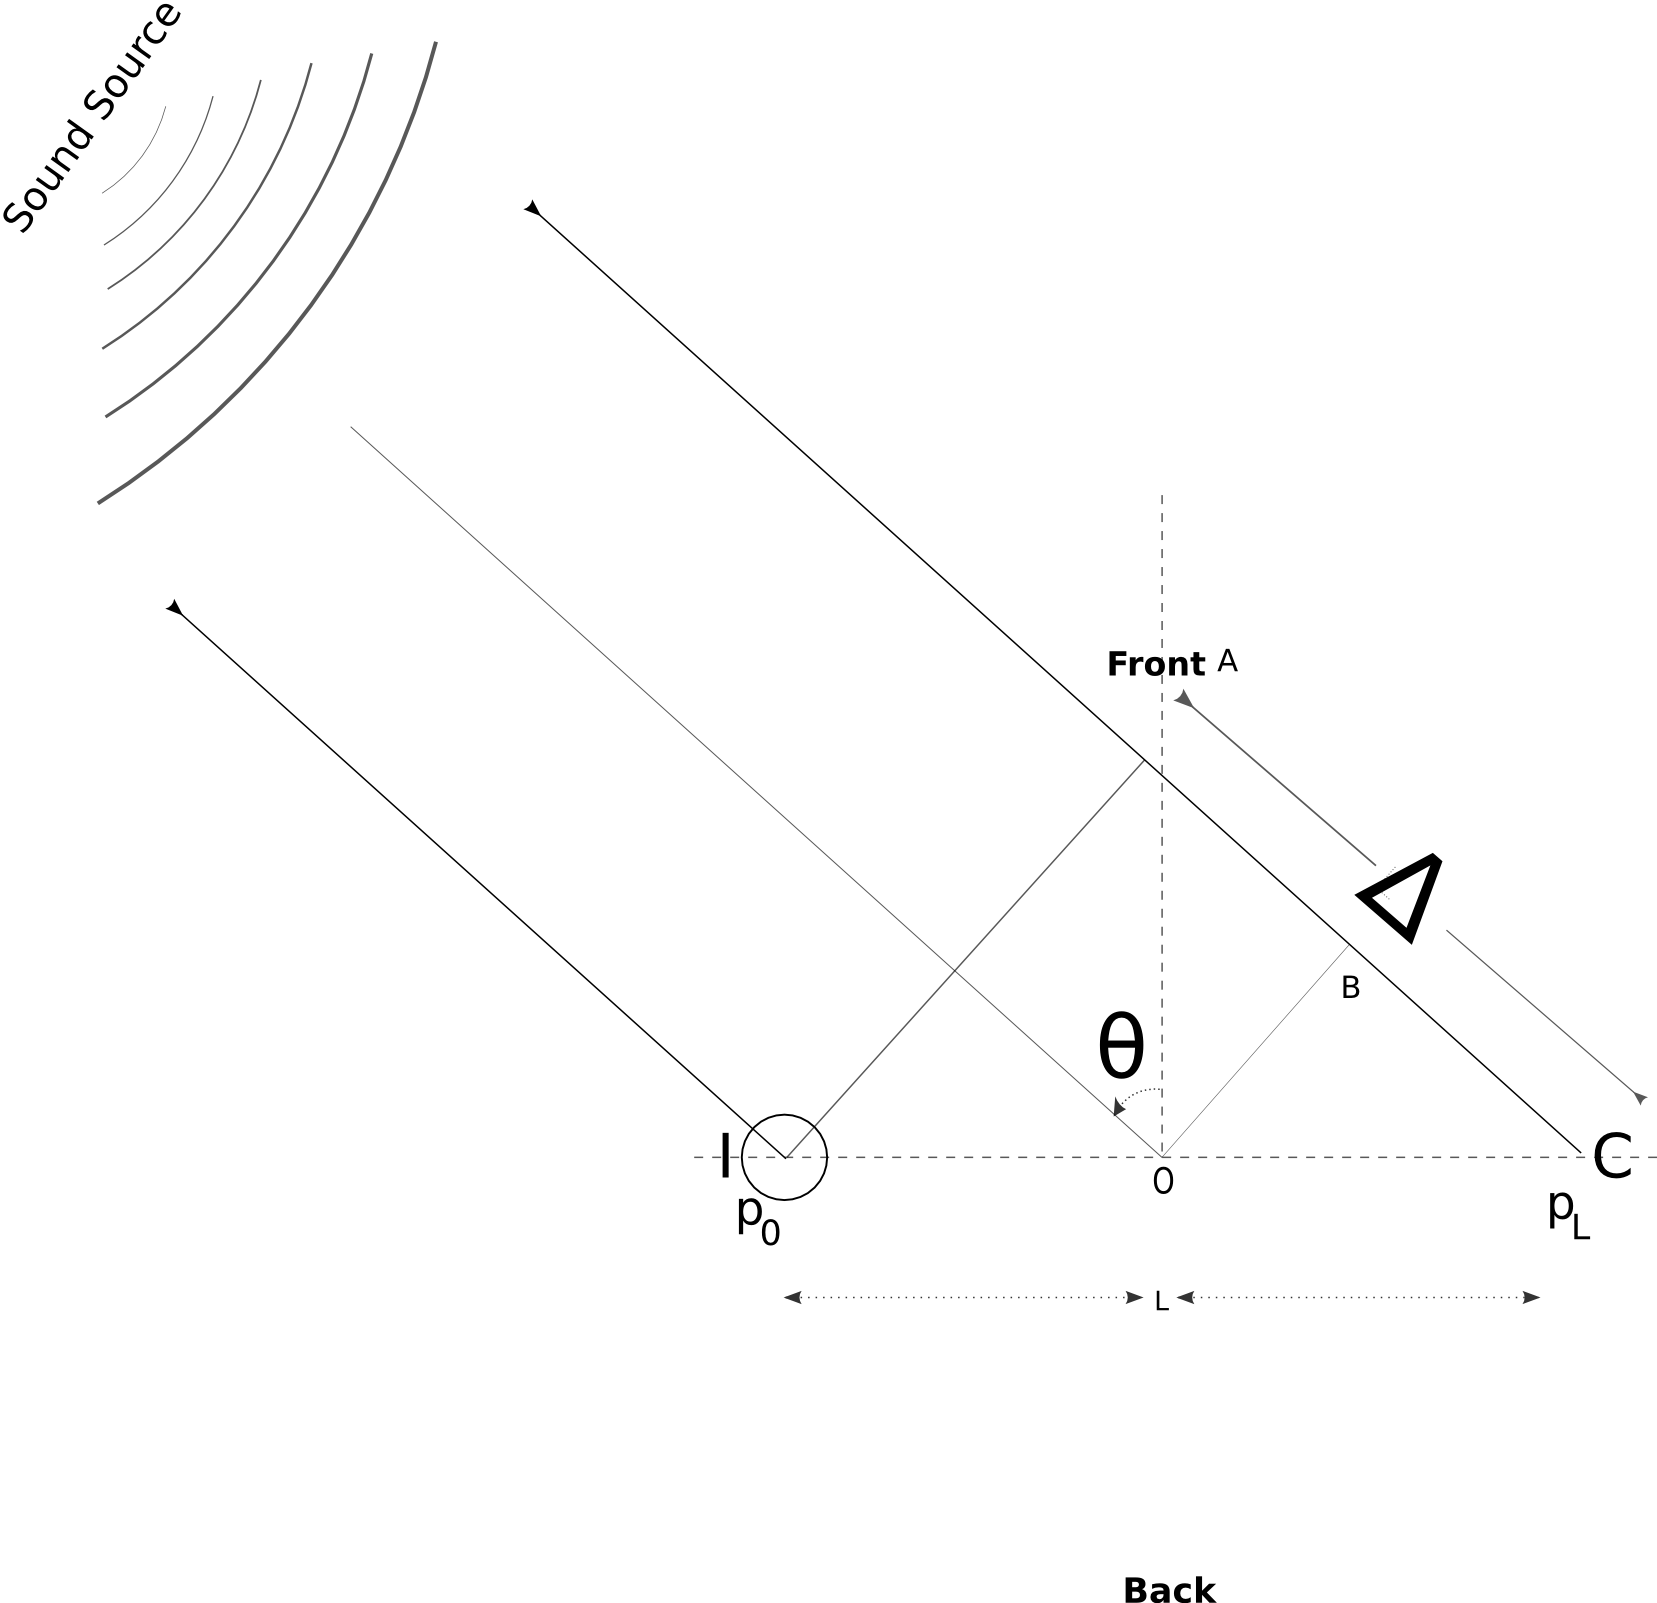
\includegraphics[width = 6 cm]{Diagrams/Presentation/acousticheadmodelold.png}\\
    \end{column}

    \end{columns}
\end{frame}

\begin{frame}[t]
 \frametitle{Acoustic Head Model - new}
 \begin{columns}
     \begin{column}{.5\textwidth}
    \small
    \flushleft
%      \begin{itemize}
%       \item<1> \textbf{I} - Ipsilateral ear, \textbf{C} - Contralateral ear.
%       \item<1>  $p_0,\ p_L$ - sound pressure on eardrums,
%       $\theta$ - sound source direction.
%      \end{itemize}
     \begin{itemize}
      \item[$\bullet$] $|p_0|=|p_L|$.
      \item[]
      \item $\Delta=\frac{3}{2}kL\sin\theta$.
      \item[]
      \item[$\bullet$] $p_0=\mbox{p}\mathrm{ exp}\left(-j\Delta/2\right)$\\ $p_L=\mbox{p}\mathrm{ exp}\left(j\Delta/2\right)$
  %    \item[]
      \item[$\bullet$] ILD=0, ITD$=\frac{3}{2}$L/c
      \end{itemize}
    \end{column}
    
 \begin{column}{0.5\textwidth}
%     \centering
%     \small
%     \underline{\textbf{Head Model}}\\
%     \flushleft
    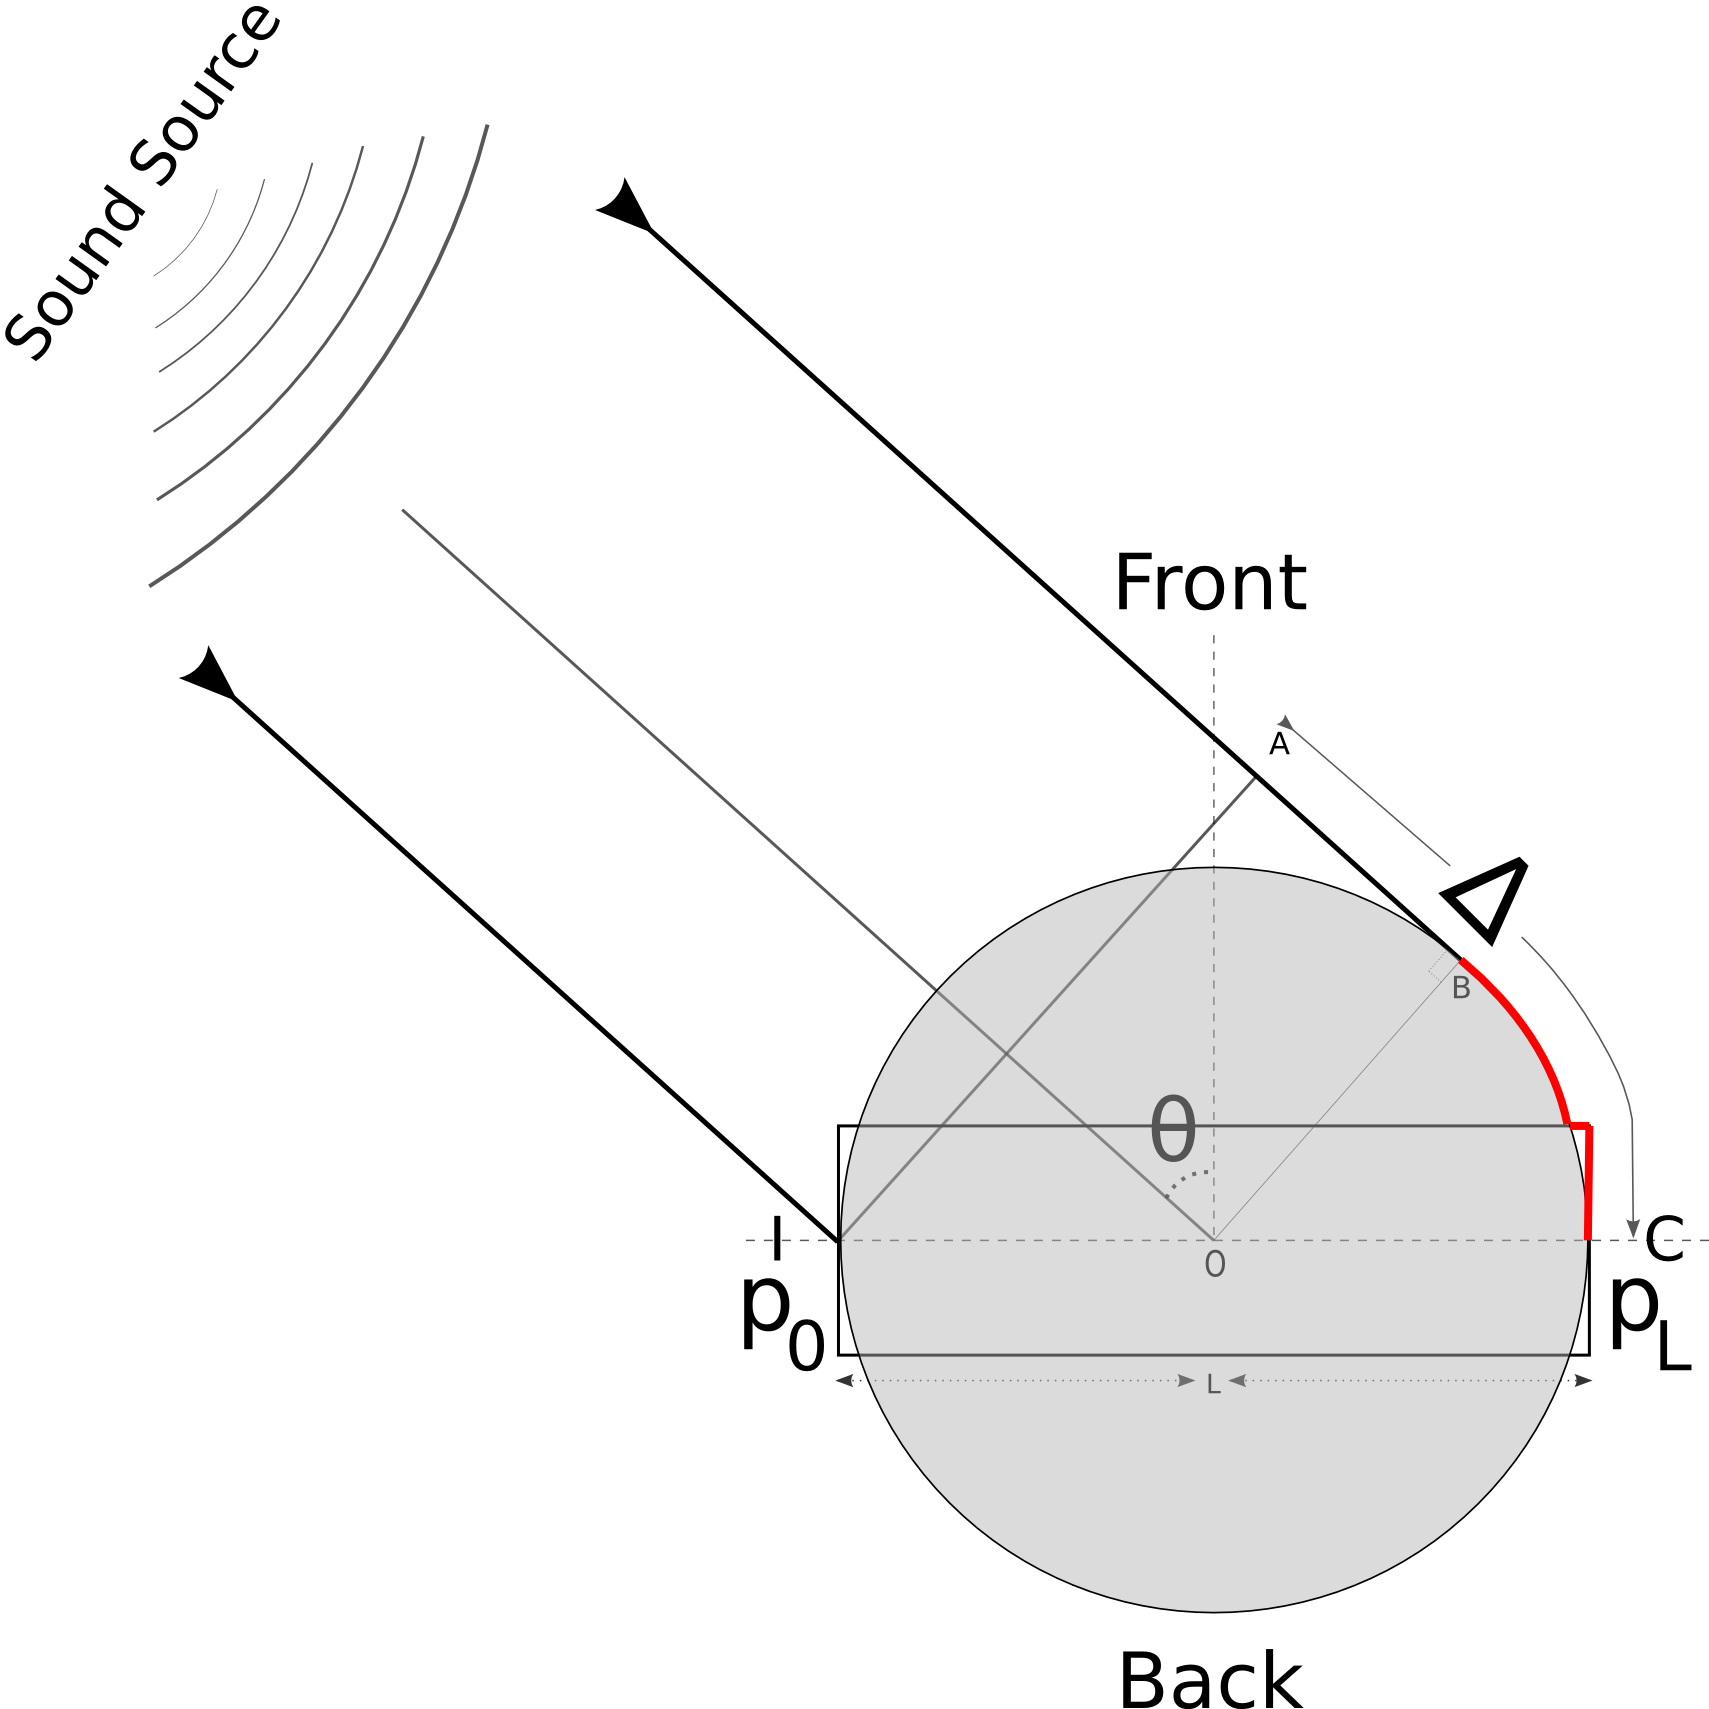
\includegraphics[width = 6 cm]{Diagrams/Presentation/acousticheadmodel2.png}\\
    \end{column}

    \end{columns}
\end{frame}

\subsection{Coupled Membranes}
\subsubsection{Ansatz}
\begin{frame}
 \frametitle{Coupled Membranes}
 \onslide<1->{\begin{variableblock}{}{bg= blue!5,fg=black}{bg= blue!5,fg=blue!75}
  \begin{equation*}
  u_{0/L}=\displaystyle\sum^{\infty}_{m=0,n=1}C^{0/L}_{\mathrm{mn}}u_{\mathrm{mn}}(r,\phi)e^{j\omega t}
 \end{equation*}
 \end{variableblock}
 }
\vfill
 \onslide<2->{\begin{exampleblock}{Membrane Equations}
%   \begin{align*}
%  &\displaystyle\sum^{\infty}_{m=0,n=1}\Omega_{\mathrm{mn}}C^0_{\mathrm{mn}}u_{\mathrm{mn}}(r,\phi)e^{j\omega t}=p_0e^{j\omega t}-p(0,r,\phi;t)\\
%  &\displaystyle\sum^{\infty}_{m=0,n=1}\Omega_{\mathrm{mn}}C^L_{\mathrm{mn}}u_{\mathrm{mn}}(r,\phi)e^{j\omega t}=p_{L}e^{j\omega t}-p(L,r,\phi;t)
%  \end{align*}
  \begin{align*}
 -\partial^2_tu_0-2\alpha\partial_t u_0+c^2_m \Delta_{(2)}u_0&=\frac{1}{\rho_m d}\left[p_0e^{j\omega t}-p(0,r,\phi;t)\right]\\
 -\partial^2_tu_L-2\alpha\partial_t u_L+c^2_m \Delta_{(2)}u_L&=\frac{1}{\rho_m d}\left[p_Le^{j\omega t}-p(L,r,\phi;t)\right]
 \end{align*}
 %-\partial^2_tu-2\textcolor{red}{\alpha}\partial_t u+\textcolor{blue}{c}^2_{\textcolor{blue}{m}} \Delta_{(2)}u=\frac{1}{\textcolor{red}{\rho_m} \textcolor{blue}{d}}\Psi(r,\phi;t)
\end{exampleblock}}

\end{frame}

\subsubsection{Boundary Conditions}
% \begin{frame}
%   \begin{exampleblock}{``Surface'' Velocity}
%  \begin{equation*}
%  U_{0/L}=\begin{cases}
%           u_{0/L}\mbox{, } 0<r<a_{\mathrm{tymp}}\mbox{ and } \beta<\phi<2\pi-\beta\\
%           0\mbox{, otherwise}
%          \end{cases}.
% \end{equation*}
% \end{exampleblock}
%  \begin{variableblock}{Velocity in $x-$direction}{bg= blue!5,fg=black}{bg= blue!5,fg=blue!75}
%   \begin{equation*}
% v_x=-\displaystyle\sum^\infty_{q=0,s=0}\frac{\zeta_{\mathrm{qs}}}{\rho\omega}\left(A_{\mathrm{qs}}e^{j\zeta_{\mathrm{qs}}x}-B_{\mathrm{qs}}e^{-j\zeta_{\mathrm{qs}}x}\right)p_{\mathrm{qs}}(r,\phi)e^{j\omega t}
% \end{equation*}
%  \end{variableblock}
% 
% \end{frame}

\begin{frame}
 \frametitle{Boundary Conditions}
  \onslide<1>{\begin{exampleblock}{Exact}
  \begin{columns}
  \begin{column}{.5\textwidth}
  \begin{align*}
 u_{0}&=-\frac{1}{j\omega}v_x(0,r,\phi;t)\nonumber\\
  u_{L}&=\frac{1}{j\omega}v_x(L,r,\phi;t)\nonumber
 \end{align*}
 \end{column}
 
   \begin{column}{.5\textwidth}
   %\centering
\includegraphics<1>[width=5.2cm]{Diagrams/Presentation/BoundaryConditions/velocity1.png}
 \end{column}
 \end{columns}

 \end{exampleblock}}
 
 \onslide<2>{\begin{variableblock}{Approximate -  $S^{0/L}(t)=\vcentcolon(\pi a^2_\mathrm{cyl})^{-1}\int dSu_{0/L}$}{bg= blue!5,fg=black}{bg= blue!5,fg=blue!75}
 
   \begin{columns}
  \begin{column}{.5\textwidth}
  \begin{align*}
 \mathbin{\textcolor{blue}{S^0}}&=-\frac{1}{j\omega}v_x(0,r,\phi;t)\nonumber\\
 \mathbin{\textcolor{blue}{S^L}}&=\frac{1}{j\omega}v_x(L,r,\phi;t)\nonumber
 \end{align*}
 \end{column}
 
   \begin{column}{.5\textwidth}
   %\centering
\includegraphics<2>[width=5.2cm]{Diagrams/Presentation/BoundaryConditions/velocity2.png}
 \end{column}
 \end{columns}
  \end{variableblock}}
\end{frame}
\subsubsection{Solution}
\begin{frame}
 \frametitle{Average Velocity}
\begin{exampleblock}{}
%$\int dS\mbox{p}_{qs}=0\Rightarrow$ 
Higher pressure modes disappear, i.e. \[p=\left[A_{00}e^{jkx}+B_{00}e^{-jkx}\right]e^{j\omega t}\]

 \begin{align*}
 &\left(\Lambda-\frac{\rho\omega^2}{k\tan kL}\right)S^0-\frac{\rho\omega^2}{k\sin kL}S^L=p_{0}\\
 &\left(\Lambda-\frac{\rho\omega^2}{k\tan kL}\right)S^L-\frac{\rho\omega^2}{k\sin kL}S^0=p_{L}
\end{align*}
% \begin{align*}
%  A_{00}&=-\frac{\rho\omega^2}{2 k\sin kL}\left(S^0e^{-jkL}+S^L\right)\\ 
%  B_{00}&=-\frac{\rho\omega^2}{2 k\sin kL}\left(S^0e^{jkL}+S^L\right)
% \end{align*}
\end{exampleblock}
 
  \onslide<2->{\begin{exampleblock}{}
\[\frac{1}{\Lambda}=\frac{1}{\pi a^2_{\mathrm{cyl}}}\displaystyle\sum^\infty_{m=0,n=1}\frac{\left(\int dS u_{\mathrm{mn}}\right)^2}{\Omega_{\mathrm{mn}}\int dS u^2_{\mathrm{mn}}}\]
\end{exampleblock}}


\end{frame}

% \begin{frame}
%  \onslide<1>{\begin{exampleblock}{Coupled Equations}
%  \begin{align*}
%  &\displaystyle\sum^\infty_{m=0,n=1}\Omega_{\mathrm{mn}}C^{0}_{\mathrm{mn}}u_{\mathrm{mn}}(r,\phi)=p_{0}+\frac{\rho\omega^2}{k}\left(\frac{S^0}{\tan kL}+\frac{S^L}{\sin kL}\right)\nonumber\\
%  &\displaystyle\sum^\infty_{m=0,n=1}\Omega_{\mathrm{mn}}C^{L}_{\mathrm{mn}}u_{\mathrm{mn}}(r,\phi)=p_{L}+\frac{\rho\omega^2}{k}\left(\frac{S^0}{\sin kL}+\frac{S^L}{\tan kL}\right)\nonumber
% \end{align*}
% \end{exampleblock}}
% 
% \onslide<2>{\begin{variableblock}{Decoupling - $\pm$}{bg= blue!5,fg=black}{bg= blue!5,fg=blue!75}
% \begin{align*}
%  &\displaystyle\sum^\infty_{m=0,n=1}\Omega_{\mathrm{mn}}C^{+}_{\mathrm{mn}}u_{\mathrm{mn}}(r,\phi)=p_{+}+\frac{\rho\omega^2}{k}S^+\cot \frac{kL}{2}\\
%  &\displaystyle\sum^\infty_{m=0,n=1}\Omega_{\mathrm{mn}}C^{-}_{\mathrm{mn}}u_{\mathrm{mn}}(r,\phi)=p_{-}-\frac{\rho\omega^2}{k}S^-\tan \frac{kL}{2}
% \end{align*}
%   \end{variableblock}}
% \end{frame}
% \begin{frame}
%   \begin{exampleblock}{Decoupled Equations}
% \begin{align*}
%  &\displaystyle\sum^\infty_{m=0,n=1}\Omega_{\mathrm{mn}}C^{+}_{\mathrm{mn}}u_{\mathrm{mn}}(r,\phi)=p_{+}+\frac{\rho\omega^2}{k}S^+\cot \frac{kL}{2}\\
%  &\displaystyle\sum^\infty_{m=0,n=1}\Omega_{\mathrm{mn}}C^{-}_{\mathrm{mn}}u_{\mathrm{mn}}(r,\phi)=p_{-}-\frac{\rho\omega^2}{k}S^-\tan \frac{kL}{2}
% \end{align*}
% \end{exampleblock}
% 
% \begin{variableblock}{}{bg= blue!5,fg=black}{bg= blue!5,fg=blue!75}
% \begin{align*}
%  C^{+}_{\mathrm{mn}}&=\left[p_{+}+\frac{\rho\omega^2}{k}S^+\cot \frac{kL}{2}\right]\frac{\int dS u_{\mathrm{mn}}}{\Omega_{\mathrm{mn}}\int dS u^2_{\mathrm{mn}}}\label{pluscoeffdef}\\
%  C^{-}_{\mathrm{mn}}&=\left[p_{-}-\frac{\rho\omega^2}{k}S^-\tan \frac{kL}{2}\right]\frac{\int dS u_{\mathrm{mn}}}{\Omega_{\mathrm{mn}}\int dS u^2_{\mathrm{mn}}}\label{minuscoeffdef}
% %\mbox{where, }K_{\mathrm{mn}}&=\frac{\int dS u_{\mathrm{mn}}}{\int dS u^2_{\mathrm{mn}}}\label{Kmndef}
% \end{align*}
%   \end{variableblock}
% \end{frame}

% \begin{frame}
%  \begin{exampleblock}{Decoupled Equations contd.}
%   \begin{equation*}
%  S^{+}=\frac{p_L+p_0}{\Lambda+\Gamma_+}\qquad S^{-}=\frac{p_L-p_0}{\Lambda+\Gamma_-}
% \end{equation*}
%  \end{exampleblock}
%  \begin{variableblock}{}{bg= blue!5,fg=black}{bg= blue!5,fg=blue!75}
%  \begin{align*}
%  \Gamma_+ = &-\frac{\rho\omega^2}{k}\cot \frac{kL}{2},\qquad \Gamma_-= \frac{\rho\omega^2}{k}\tan \frac{kL}{2}\\
% &\frac{1}{\Lambda}=\frac{1}{\pi a^2_{\mathrm{cyl}}}\displaystyle\sum^\infty_{m=0,n=1}\frac{\left(\int dS u_{\mathrm{mn}}\right)^2}{\Omega_{\mathrm{mn}}\int dS u^2_{\mathrm{mn}}}
% \end{align*}
% \end{variableblock}
% \end{frame}

\begin{frame}
\frametitle{Final Expressions}
 \begin{exampleblock}{Membrane Displacement}
  \begin{align*}
 S_0(t)&=G^s_{ipsi}p_0+G^s_{cont}p_L\\
 S_L(t)&=G^s_{cont}p_0+G^s_{ipsi}p_L
\end{align*}
 \end{exampleblock}

\begin{variableblock}{}{bg= blue!5,fg=black}{bg= blue!5,fg=blue!75}
\begin{columns}
 \begin{column}{.6\textwidth}
 \begin{align*}
 G^s_{ipsi}&=\frac{1}{2}\left(\frac{1}{\Lambda+\Gamma_+}+\frac{1}{\Lambda+\Gamma_-}\right) \\
 G^s_{cont}&=\frac{1}{2}\left(\frac{1}{\Lambda+\Gamma_+}-\frac{1}{\Lambda+\Gamma_-}\right)
\end{align*}
\end{column}
\begin{column}{.4\textwidth}
\centering
\begin{align*}
&\Gamma_+= -\frac{\rho\omega^2}{k}\cot \frac{kL}{2}\\
&\Gamma_-= \frac{\rho\omega^2}{k}\tan \frac{kL}{2}
\end{align*}
\end{column}
\end{columns}
\end{variableblock}

\end{frame}
% \subsection{Circuit Model}
% \begin{frame}[t]
% \frametitle{Circuit Model}
% \begin{columns}
%      \begin{column}{0.5\textwidth}
% \centering
% \underline{\textbf{High Frequency}}
% \vspace{2pt}
% \end{column}
% \begin{column}{0.5\textwidth}
% \centering
%  \underline{\textbf{Low Frequency}}
%  \vspace{2pt}
% \end{column}
% \end{columns}
% 
%   \begin{columns}
%      \begin{column}{0.5\textwidth}
%      \centering
%  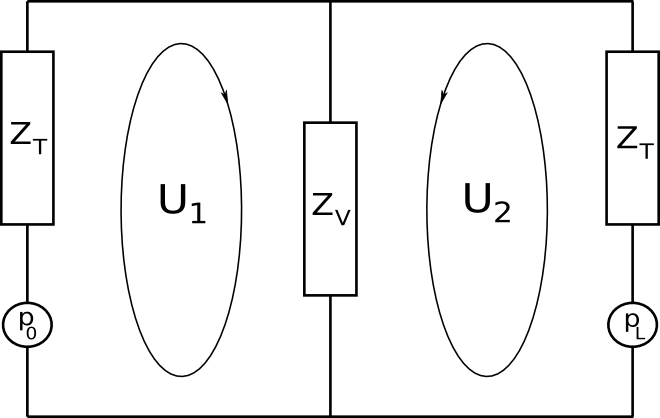
\includegraphics[width=.65\linewidth]{Diagrams/lowfreqcircuit.png}
%  \begin{variableblock}{}{bg= blue!5,fg=black}{bg= blue!5,fg=blue!75}
%  \begin{itemize}
%  \footnotesize
%   \item $Z_T$ - tympanum impedance
%   \item $Z_V$ - Cavity impedance
%  \end{itemize}
% \end{variableblock}
%      \end{column}
%      \begin{column}{0.5\textwidth}
%      \centering
%  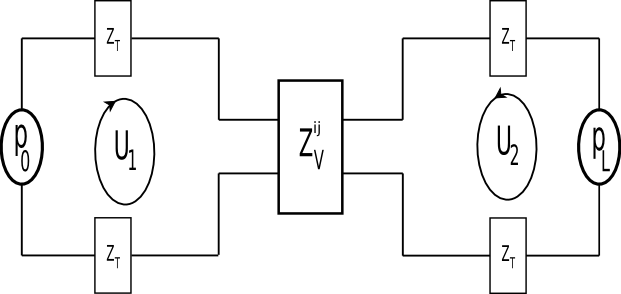
\includegraphics[width=.9\linewidth]{Diagrams/highfreqcircuit.png}
%  \begin{variableblock}{}{bg= blue!5,fg=black}{bg= blue!5,fg=blue!75}
%  \begin{itemize}
%  \footnotesize
%   \item $Z_T$ - tympanum impedance
%   \item $Z^{ij}_V$ - Cavity impedance
%  \end{itemize}
% \end{variableblock}
%      \end{column}
%      \end{columns}
%      \begin{columns}
%      \begin{column}{0.6\textwidth}
%      \begin{exampleblock}{}
%      \begin{itemize}
%       \item U$_{1/2}\equiv$Current.
%       \item $p_{0/L}\equiv$Voltage Sources.
%      \end{itemize}
%      \end{exampleblock}
%      \end{column}
%      \end{columns}
% 
% \end{frame}


\section{Evaluation}
\subsection{Parameters}
\begin{frame}[t]
 \frametitle{Tokay Gecko}
  \begin{columns}
     \begin{column}{0.5\textwidth}
     \small
 \begin{variableblock}{}{bg= blue!5,fg=black}{bg= blue!5,fg=blue!75}
\begin{tabular}{l  l}
L=$22\,$mm & $a_{\mathrm{tymp}}$=$2.6\,$mm\\
&\\
$\textcolor{red}{c_m}=5.41\,$ms$^{-1}$ & $\rho_m$=$1\,$mg/mm$^3$\\ 
&\\
$d$=$10\,\mu$m & $V_{\mathrm{\mathrm{cav}}}$=$3.5\,$ml\\ 
&\\
$\beta$=$\pi/25$&$\textcolor{blue}{a_{cyl}}\approx 6.6\,$mm \\
&\\
$\textcolor{red}{\alpha}\approx2474\ \mbox{s}^{-1}$ &\\
\end {tabular}\par
\end{variableblock}

%\bigskip
\begin{exampleblock}{}
\begin{itemize}
\item[] $f_0=\textcolor{red}{c_m}\mu_{01}/2\pi$.
\item[] ITD = $96.21\, \mu$s.
\item[] $\textcolor{red}{\alpha}\rightarrow$ steady state.
\end{itemize}
\end{exampleblock}
     \end{column}
     
     \begin{column}{0.5\textwidth}
     \centering
       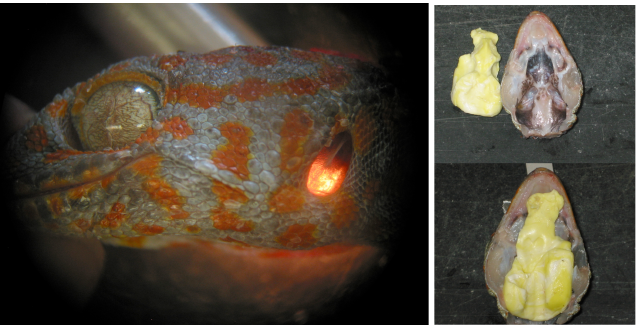
\includegraphics[width=.85\linewidth]{Diagrams/geckohead1.png}
       
      \small
      Tokay gecko. Left: Head illuminated from the opposite side\footnote{Courtesy J.C. Dalsgaard (Syddansk Universitet)}. Right: Mouth casts.
     \end{column}
  \end{columns}
\end{frame}

\subsection{Vibration Amplitude}
\begin{frame}[t]
\frametitle{Density Plot}
% \noindent Vibration Amplitude - $20\mathrm{Log}_{\mathrm{10}}\left| \dot{S}^0/\pi a^2_{\mathrm{cyl}}\right|$
\begin{variableblock}{}{bg= white,fg=black}{bg= white,fg=blue!75}
\begin{figure}[ht!]
 \centering 
 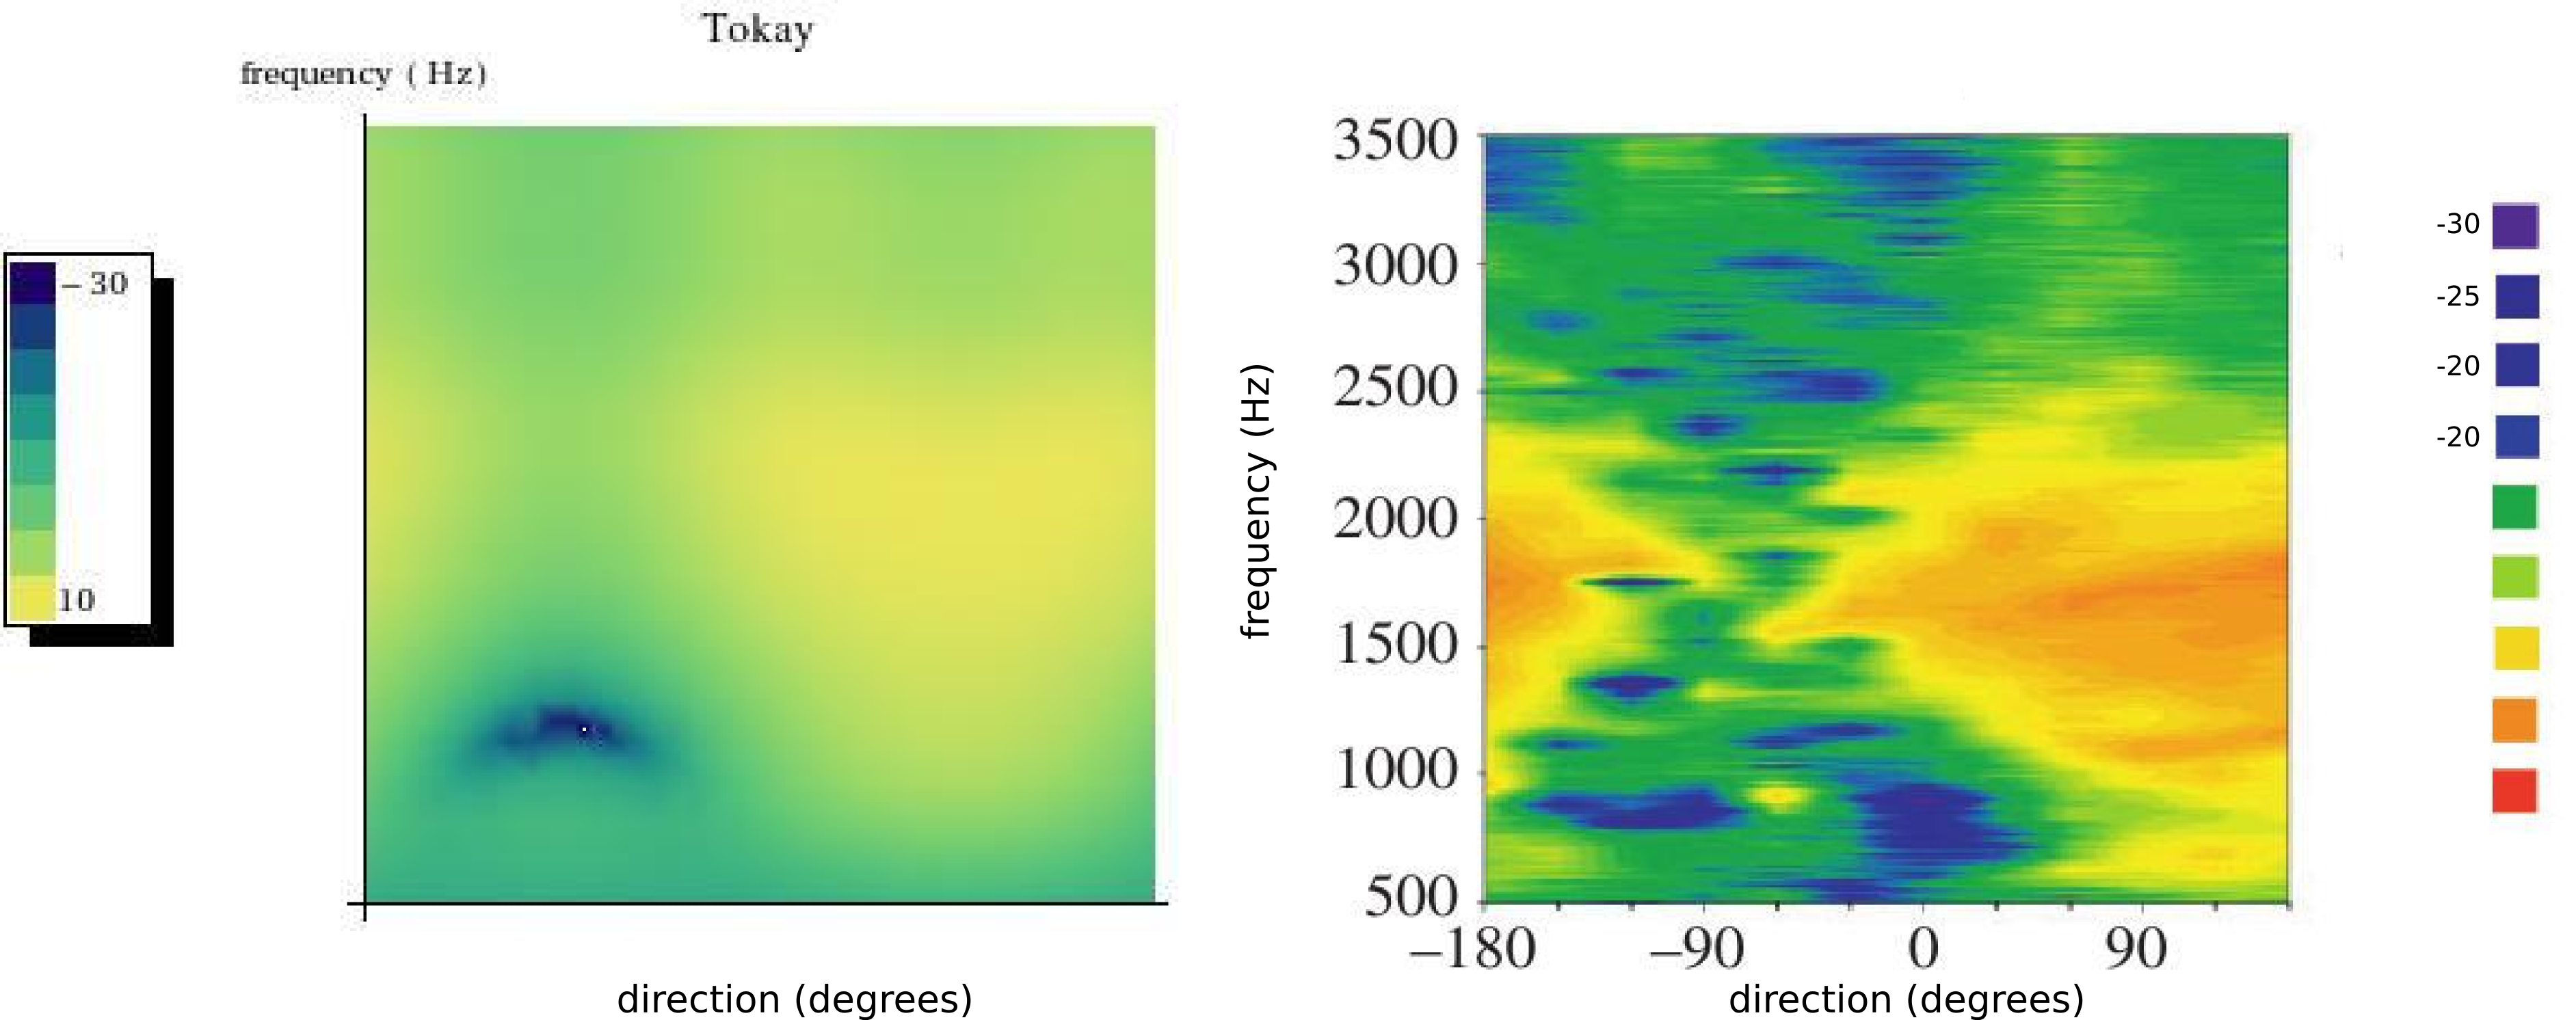
\includegraphics[width = 11 cm]{Diagrams/Plots/tokayvibampfull.png}
\end{figure}
\end{variableblock}
\begin{exampleblock}{}
\footnotesize
 \begin{itemize}
  \item Plot of vibration amplitude w.r.t direction \& frequency (Left: Calculated, Right: Experimental (Christensen-Dalsgaard et al, 2005).
  \item $\left|p_0\right|=\left|p_L\right|=1$ Pa.
 \end{itemize}
\end{exampleblock}
% \begin{columns}
%     \begin{column}{0.5\textwidth}
%       \centering
%       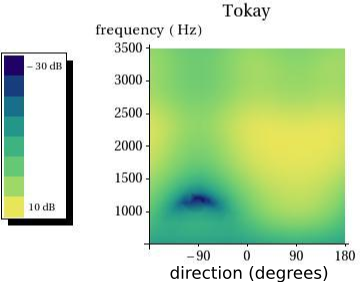
\includegraphics[width = 5.6 cm]{Diagrams/Presentation/tokayvibamp.png}\\
%      
%       \footnotesize \hspace{16pt} direction (degrees)
%     \end{column}
% 
%     \begin{column}{0.5\textwidth}
%     \textbf{}\\
%     %\textbf{}\\
%     \vspace{1pt}
%     \flushright
%       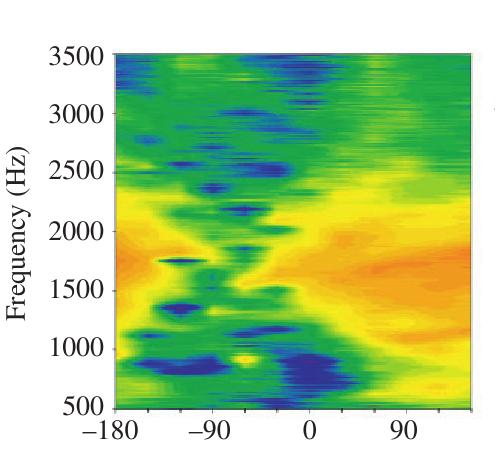
\includegraphics[width = 4.25 cm]{Diagrams/Presentation/tokayvibamp_exp.jpeg}\\
%       \centering
%       \footnotesize direction (degrees)
%     \end{column}
%   \end{columns}
\end{frame}

\begin{frame}[t]
\frametitle{Frequency Dependence}
%\noindent Frequency Dependence
\begin{variableblock}{}{bg= white,fg=black}{bg= white,fg=blue!75}
\begin{figure}[ht!]
 \centering 
 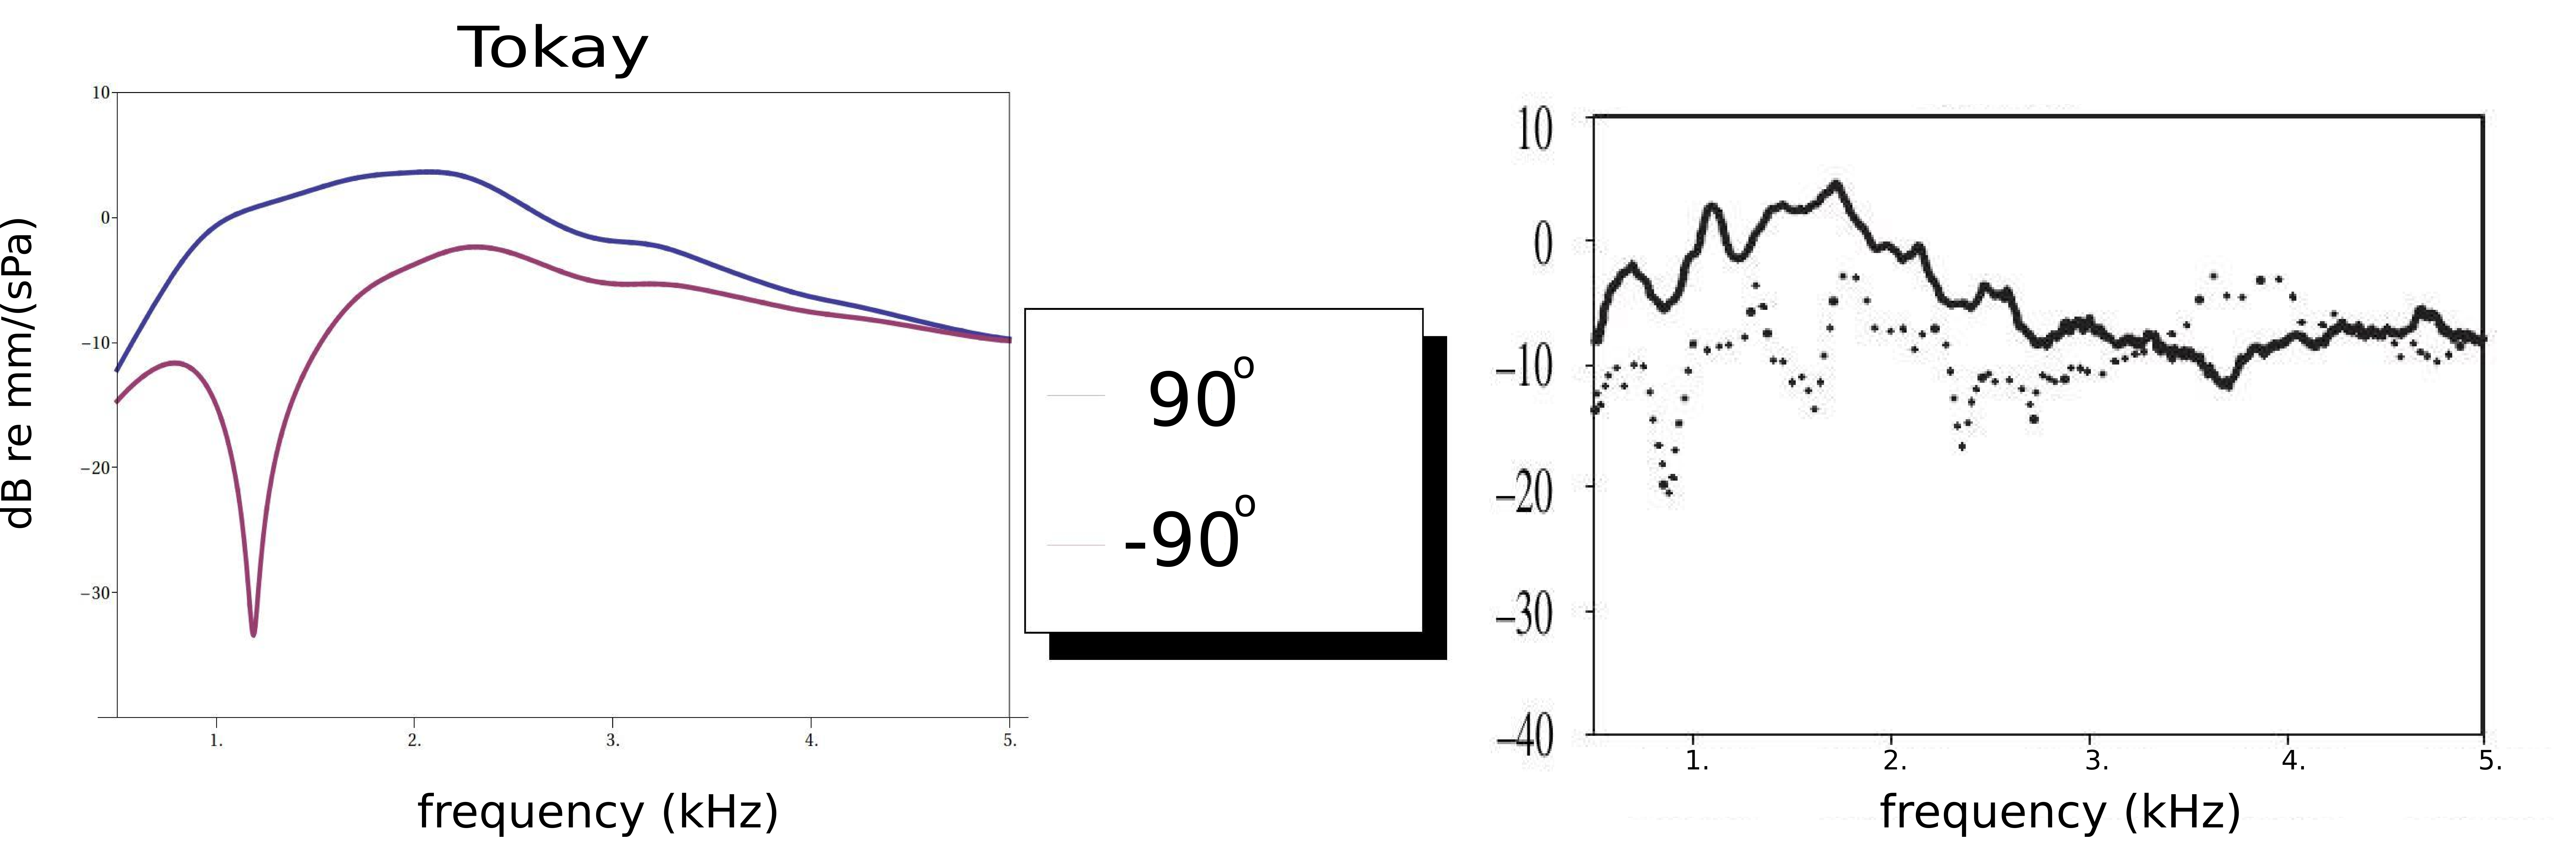
\includegraphics[width = 11 cm]{Diagrams/Presentation/tokayipsivscontrafull.png}
\end{figure}
\end{variableblock}
\begin{exampleblock}{}
\footnotesize
 \begin{itemize}
  \item Frequency dependence of $20\mathrm{Log}_{\mathrm{10}}\left| \dot{S}^0/\pi a^2_{\mathrm{cyl}}\right|$ for $\theta=90^\circ$. (Left:Calculated, Right:Experimental)
  \item $\left|p_0\right|=\left|p_L\right|=1$ Pa.
  \item Ipsilateral response $>$ Contralateral response.
 \end{itemize}
\end{exampleblock}
\end{frame}

\begin{frame}[t]
%\frametitle{Direction Dependence}
 \begin{columns}
     \begin{column}{0.45\textwidth}
     %\frametitle{Direction Dependence}
     \noindent \color{blue} Direction Dependence.
     \small
     \flushleft
\onslide<1>{\begin{exampleblock}{}
  \begin{itemize}
   \item Inputs to ears \begin{itemize}
			  \footnotesize
                         \item Negligible level (amplitude) difference
                         \item Small time (phase) difference
                        \end{itemize}
   \item Response is highly directional.

  \end{itemize}
 \end{exampleblock}}

 \vfill
 \onslide<2>{\begin{variableblock}{}{bg= blue!5,fg=black}{bg= blue!5,fg=blue!75}
	      \begin{itemize}
	       \item Independent vibration amplitudes not enough.
               \item Localization requires using information from both ears.
               \end{itemize}
              \end{variableblock}}
              \end{column}
              
              \begin{column}{0.55\textwidth}
  \only<1>{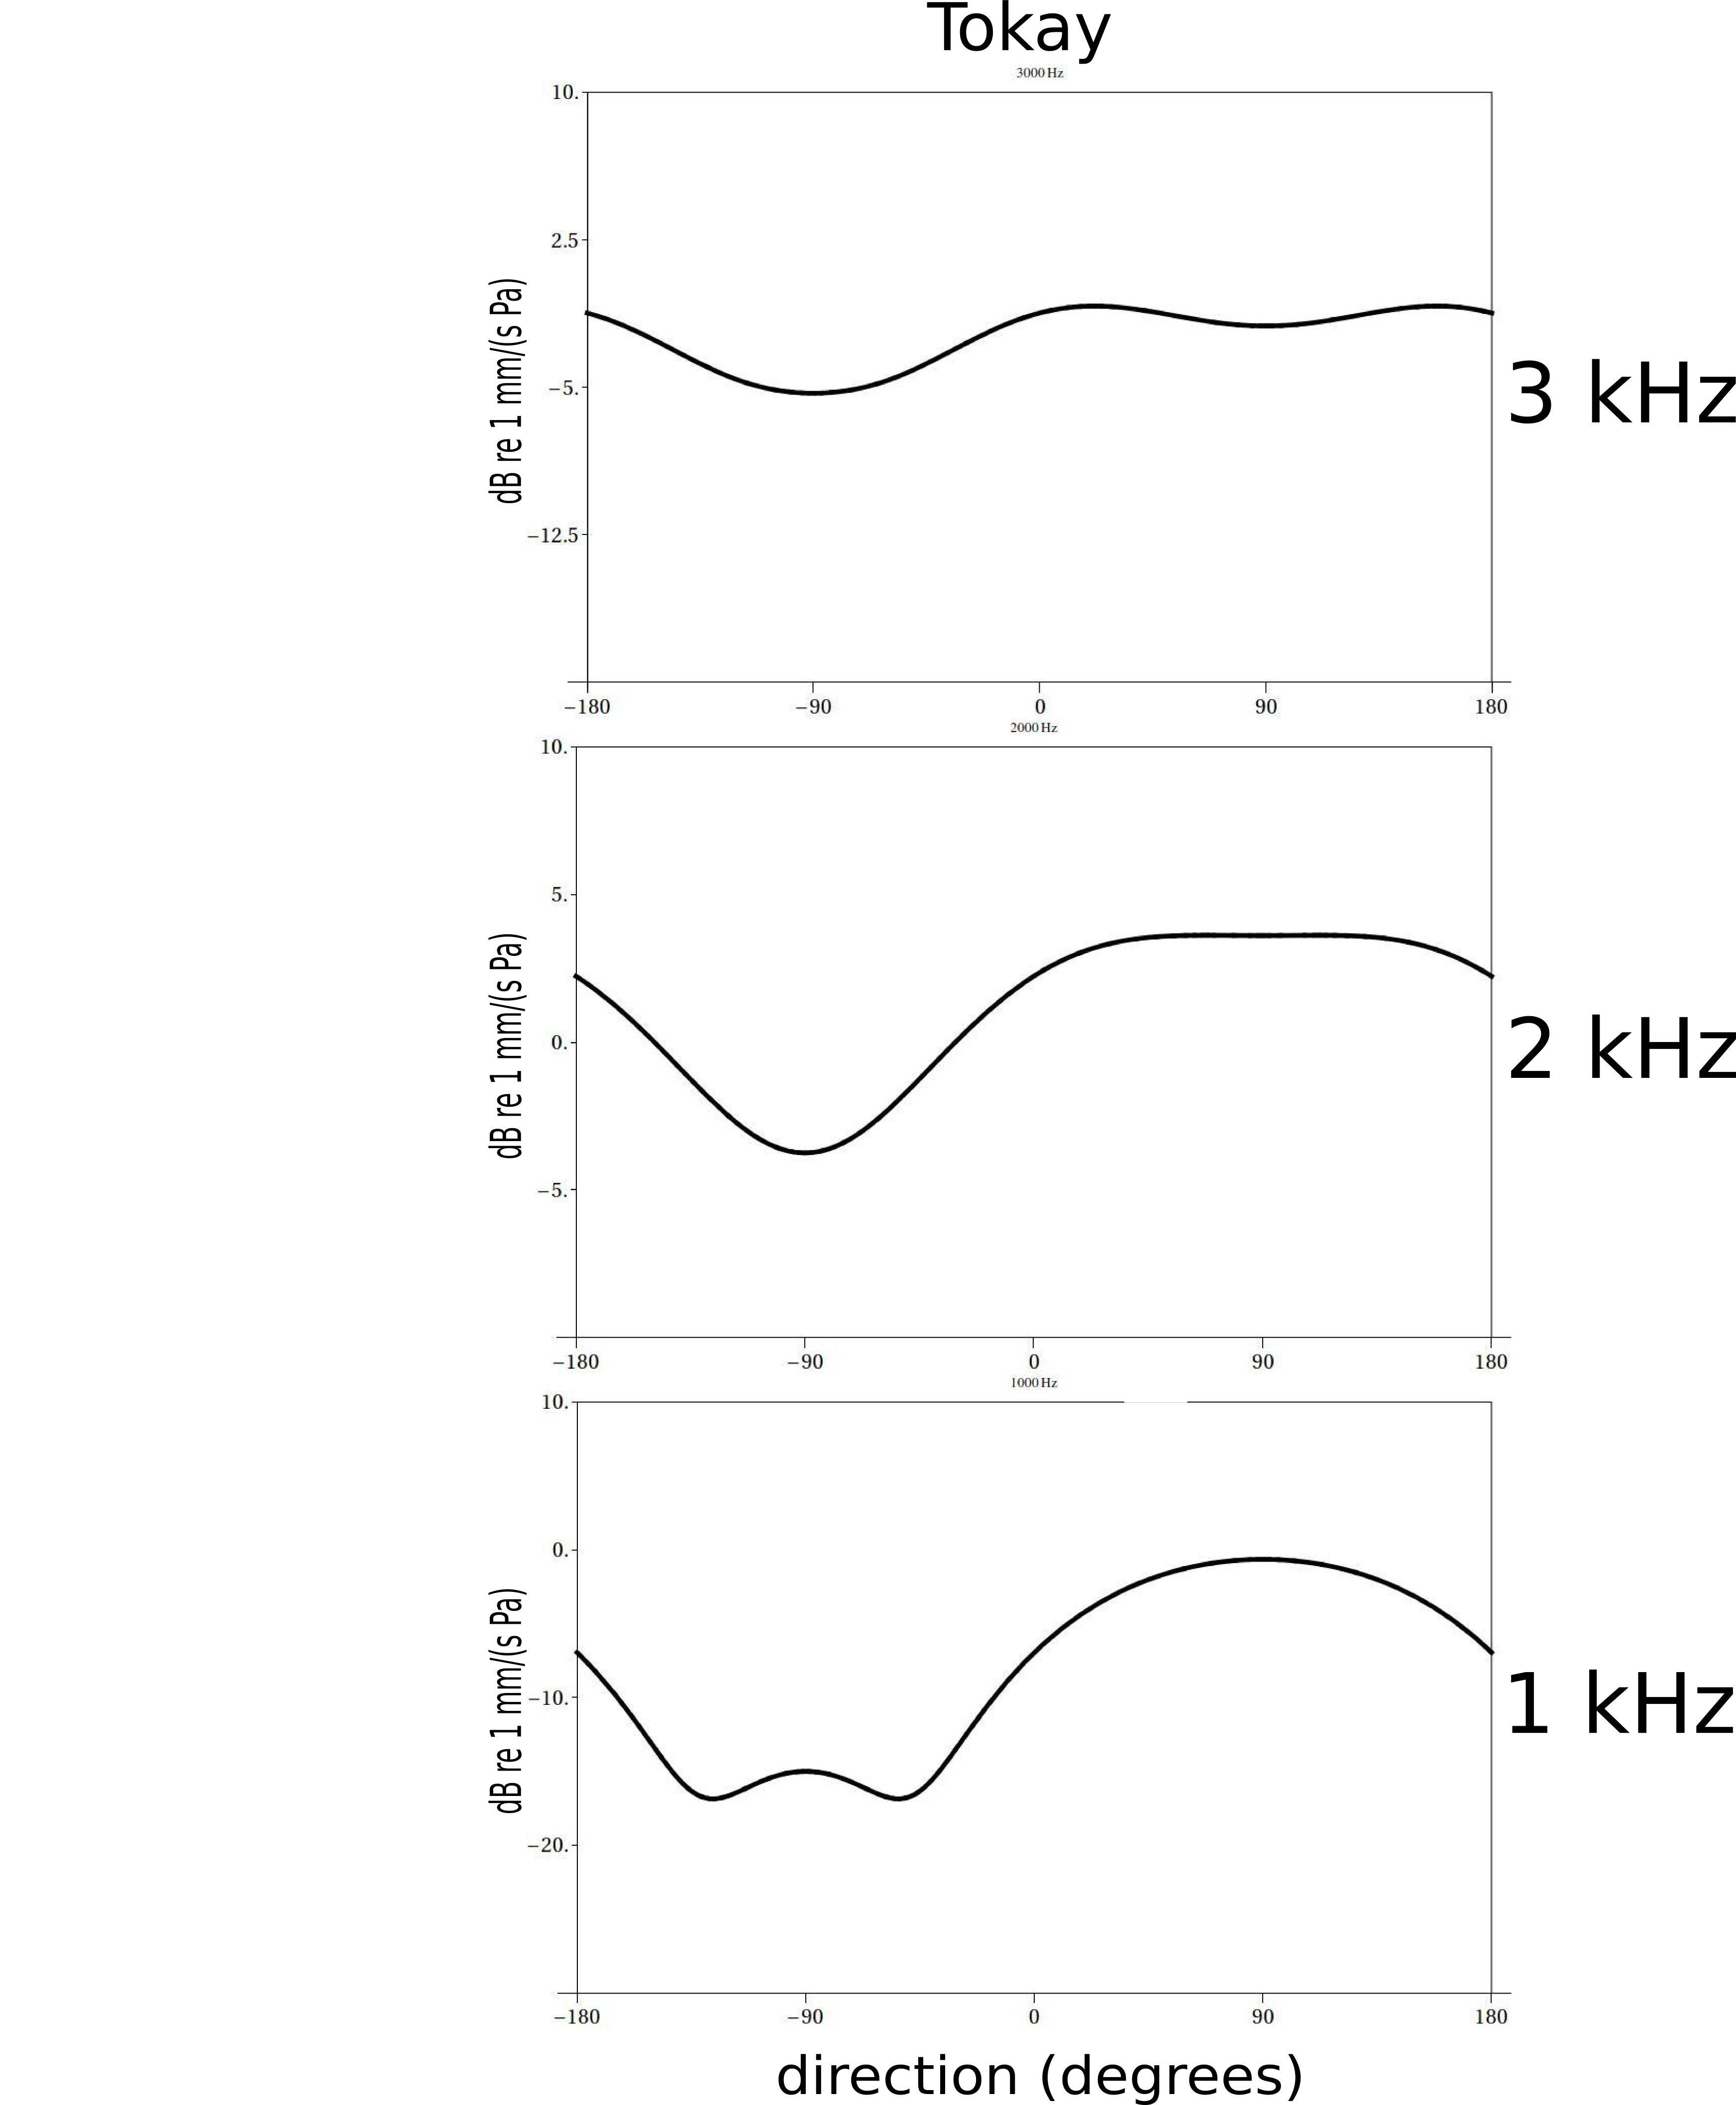
\includegraphics[width = 6.2 cm]{Diagrams/Presentation/directionplots.png}}
  %  \only<2>{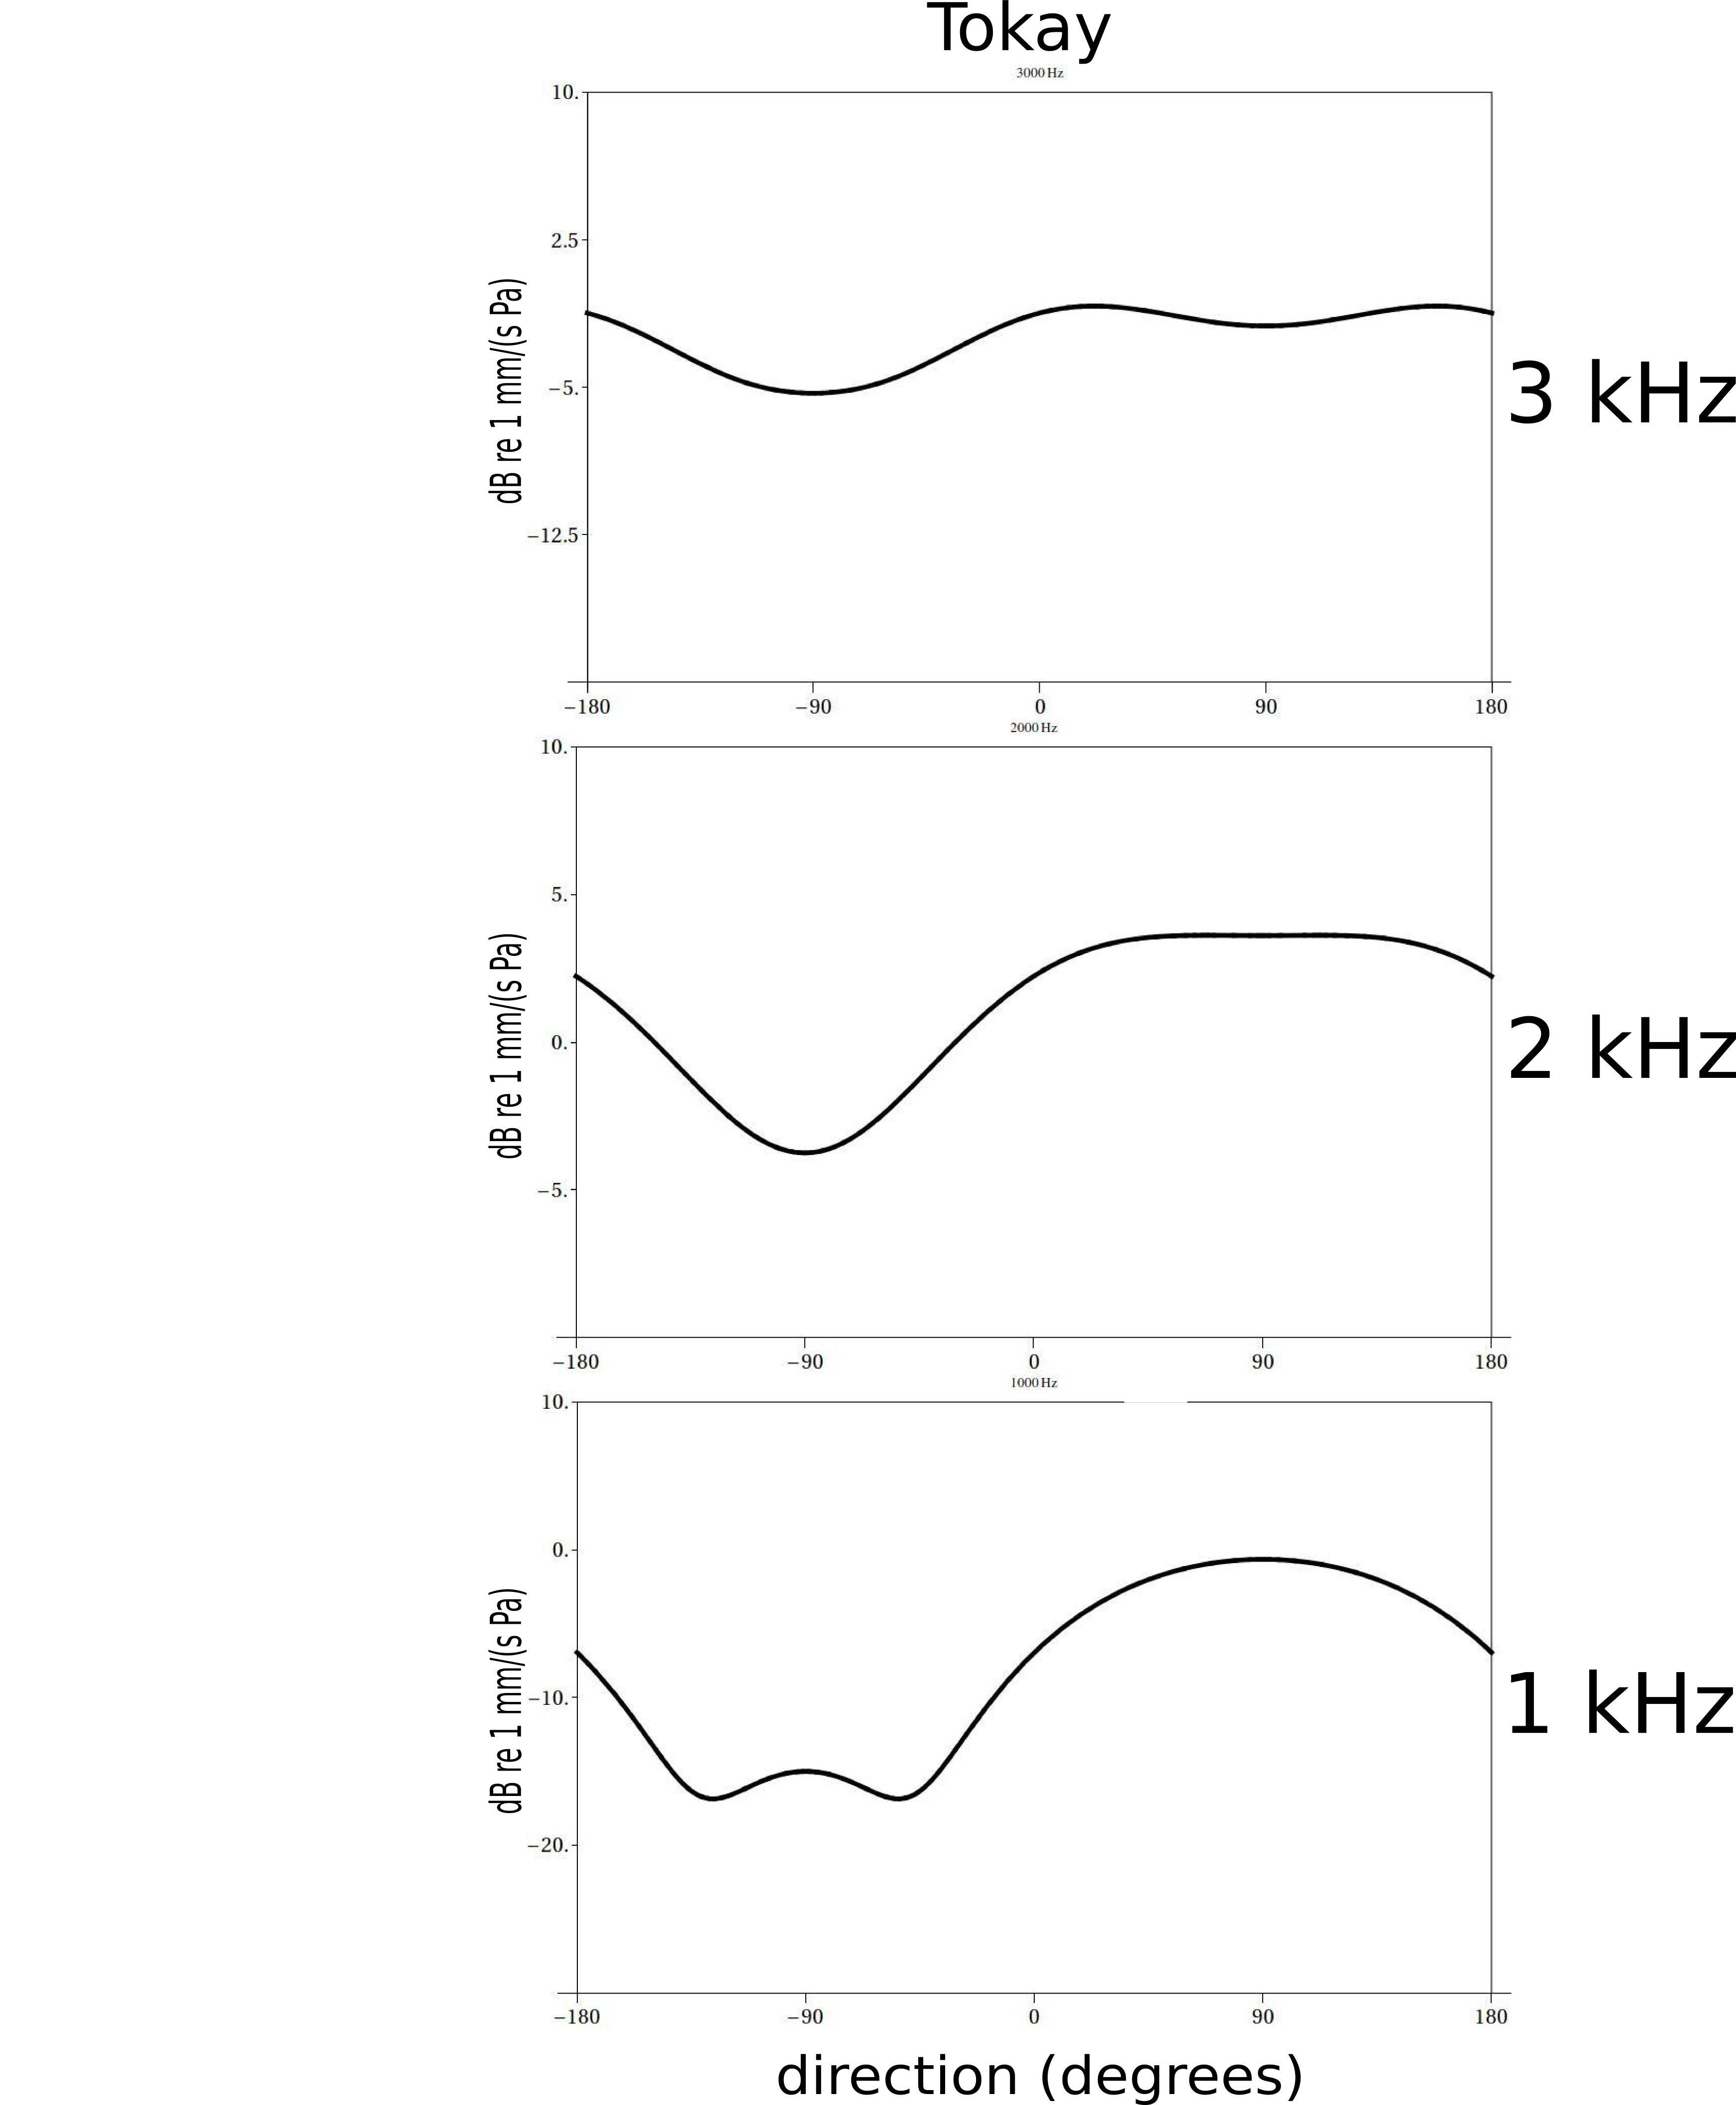
\includegraphics[width = 6.2 cm]{Diagrams/Presentation/directionplots.png}}
  \only<2>{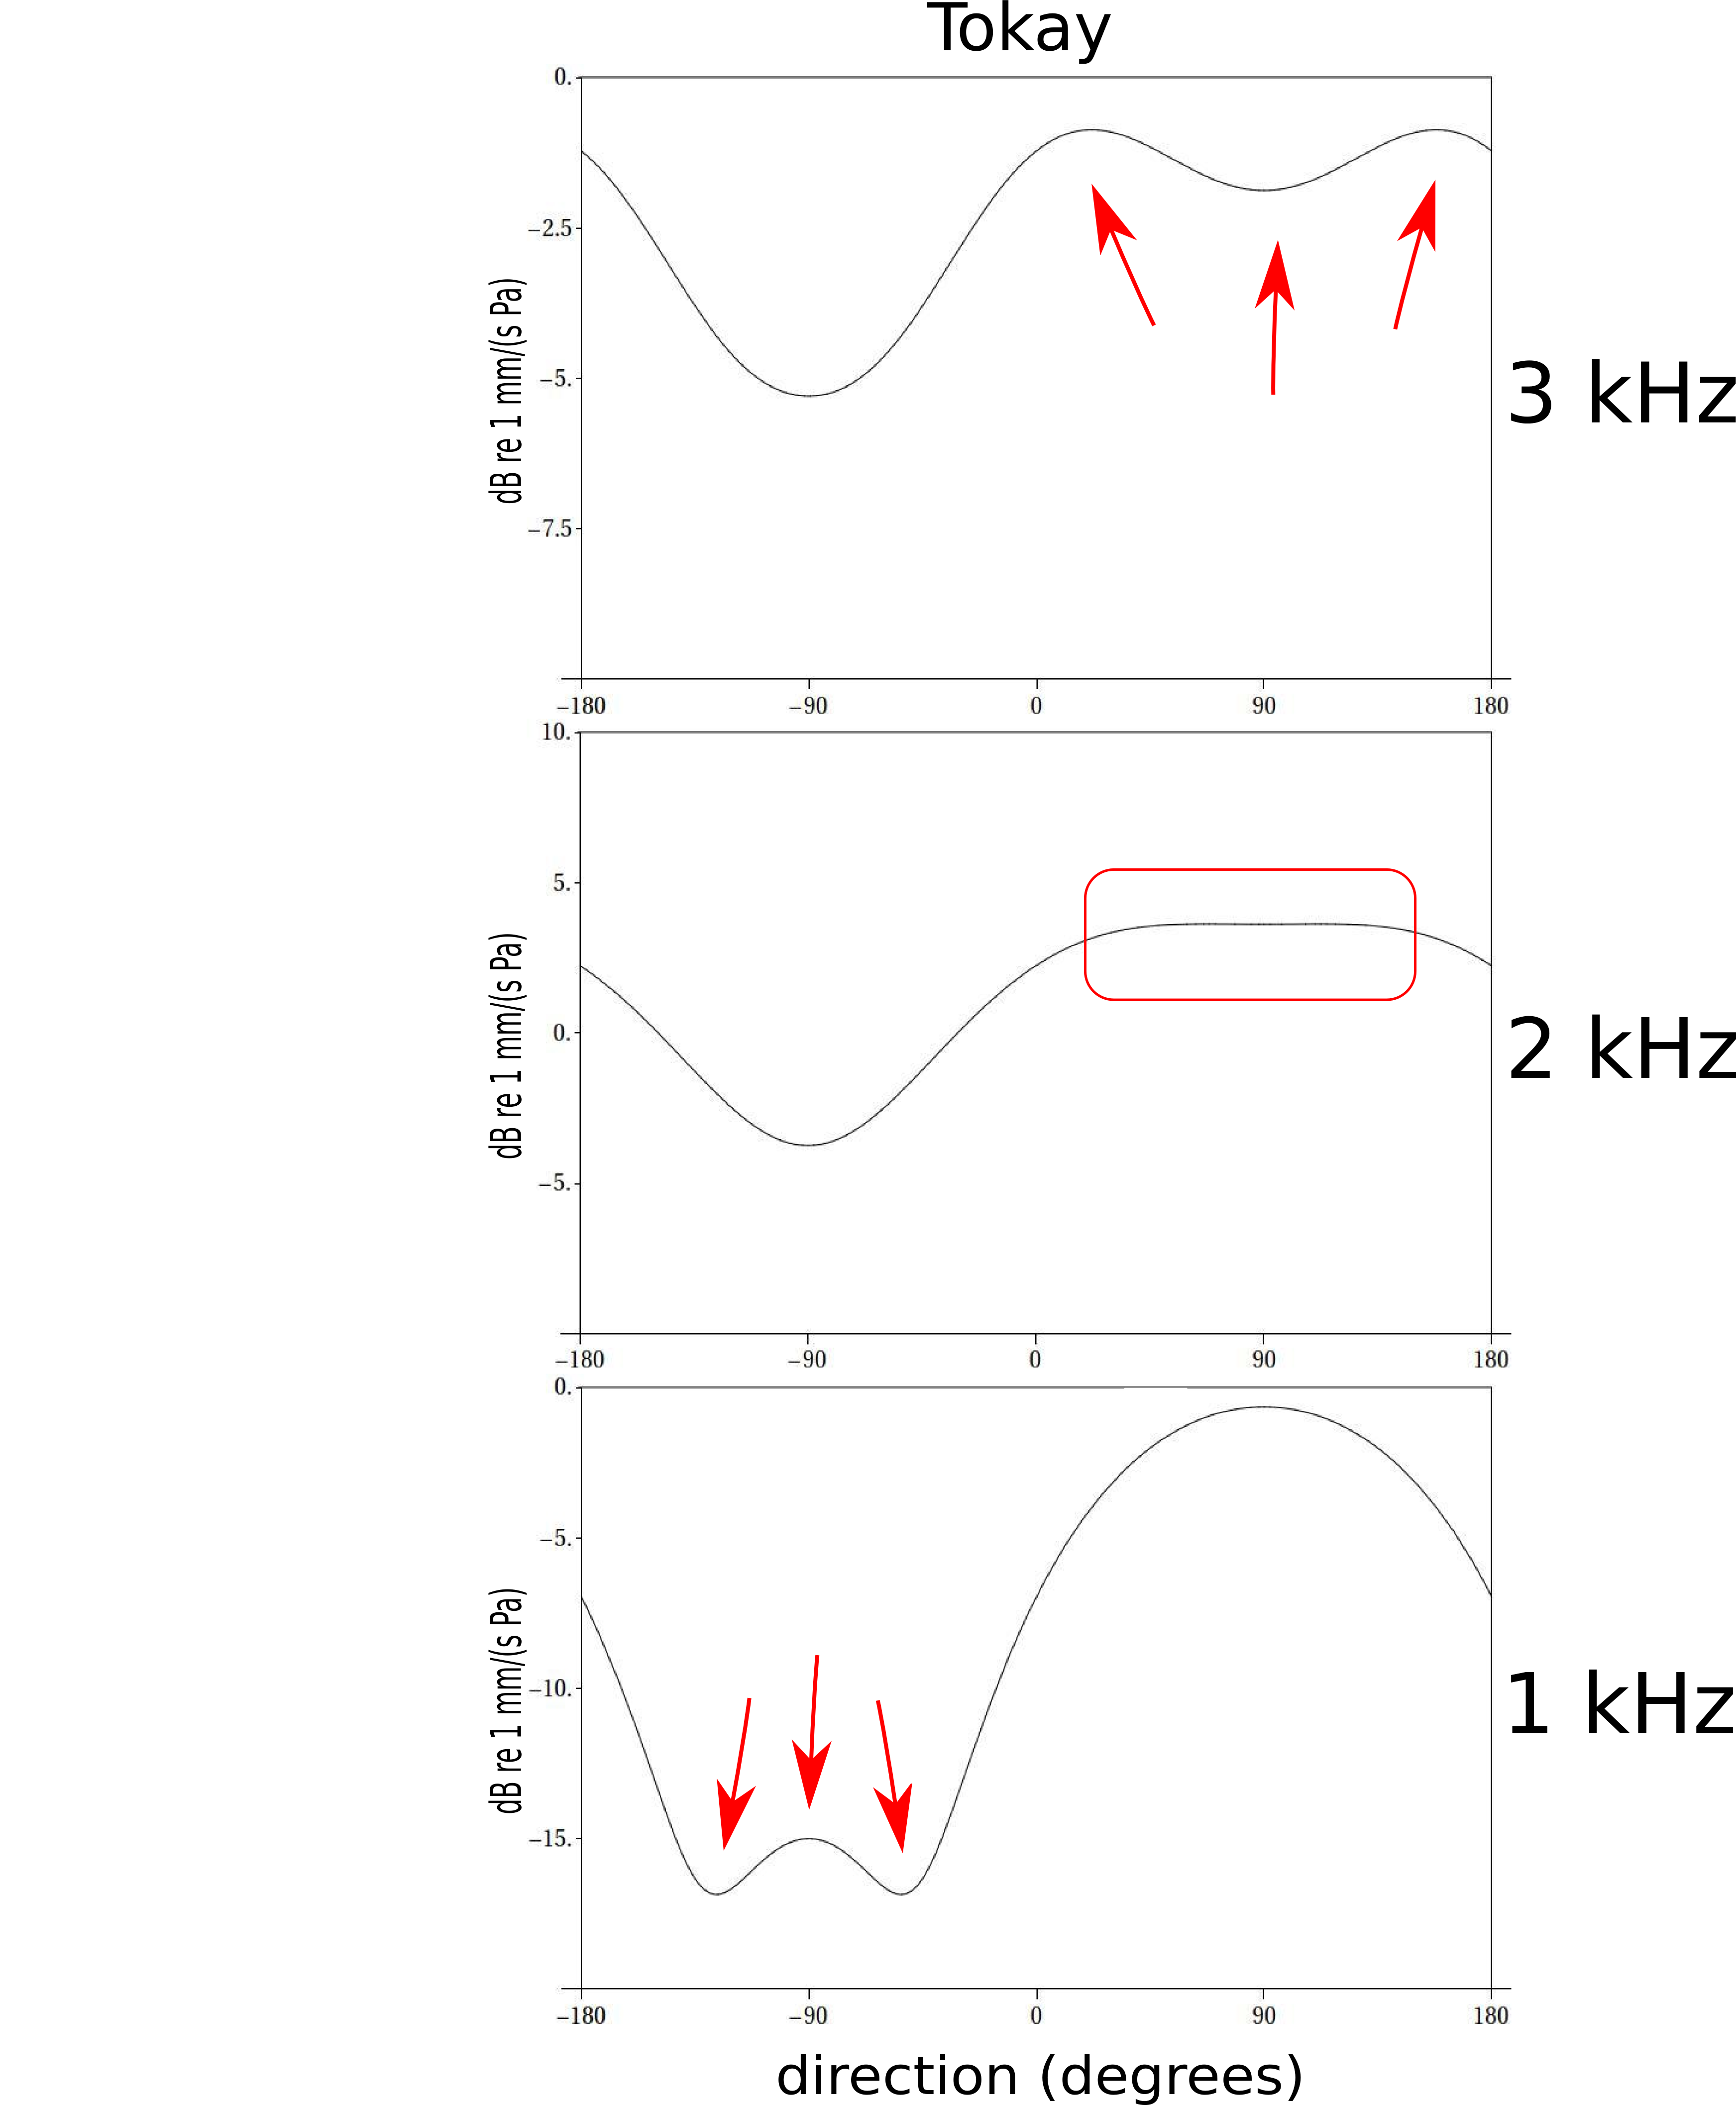
\includegraphics[width = 6.2 cm]{Diagrams/Presentation/directionplots2.png}}
\end{column}
   \end{columns}



\end{frame}
\subsection{Directional Cues}

\begin{frame}[t]
\frametitle{Hearing Cues}
 \begin{columns}
     \begin{column}{0.5\textwidth}
 \begin{variableblock}{}{bg= blue!5,fg=black}{bg= blue!5,fg=blue!75}
\onslide<1>{Internal Level Difference (iLD) - 
\begin{equation*}
  \mbox{iLD}\vcentcolon= 20\mbox{Log}_{10}\left|\frac{\dot{S}^0}{\dot{S}^L}\right|
\end{equation*}}
\onslide<1>{Internal Time Difference (iTD) - 
\begin{equation*}
 \mbox{iTD}\vcentcolon= \mbox{Arg}\left(\frac{\dot{S}^0}{\dot{S}^L}\right)/\omega
\end{equation*}}
\end{variableblock}
\end{column}
\begin{column}{0.5\textwidth}
\onslide<2>{\begin{exampleblock}{Requirements}
Both:
 \begin{enumerate}
 \small
 \item \label{listitem1} increase with the nearness of the sound source.
 \item \label{listitem3} vanish at $\theta=0^\circ,\ \pm 180^\circ$. 
\end{enumerate}
iTD:
\begin{enumerate}
\item[] $\sim$constant in a certain frequency range.
\end{enumerate}
\end{exampleblock}}
\end{column}
\end{columns}

\end{frame}


\subsubsection{Internal Level Difference}
\begin{frame}[t]
\frametitle{iLD Density Plot}
%\noindent Internal Level Difference

     \begin{variableblock}{}{bg= white,fg=black}{bg= white,fg=blue!75}
 \begin{figure}[ht!]
 \centering 
 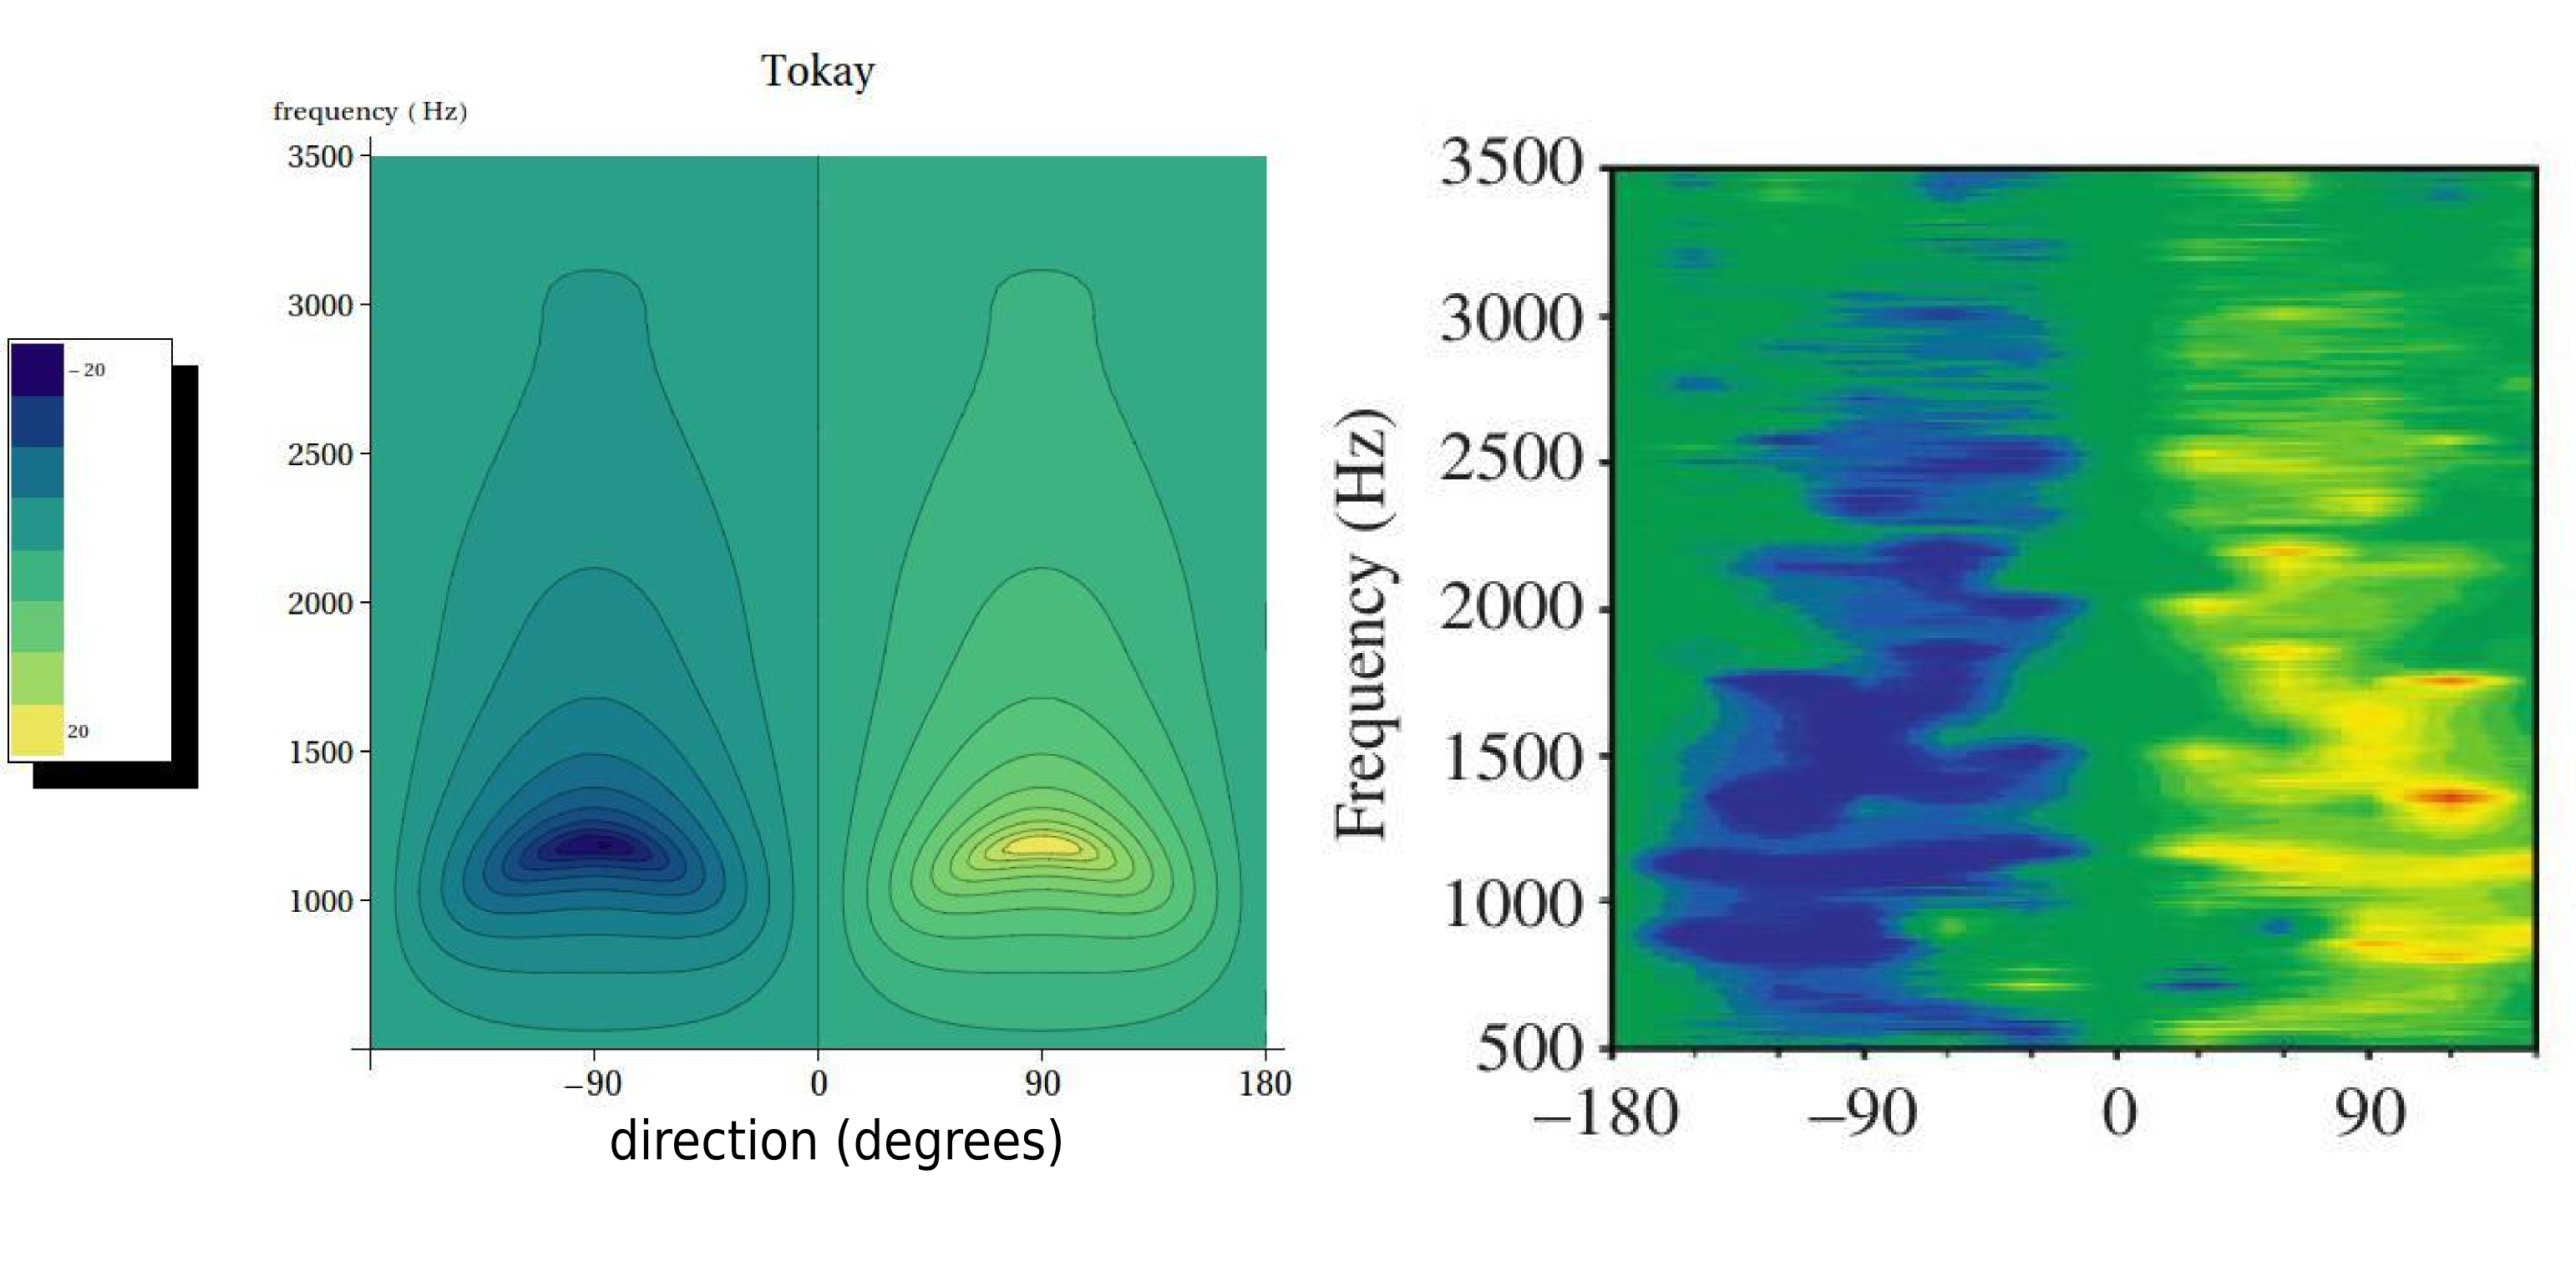
\includegraphics[width = 11 cm]{Diagrams/Plots/iLD/tokayiLDboth.png}
\end{figure}
\end{variableblock}


\begin{exampleblock}{}
\footnotesize
 \begin{itemize}
  \item Plot of iLD, against frequency and direction.
  \item Left: Calculated, Right: Experimental
 \end{itemize}
\end{exampleblock}
\end{frame}

\begin{frame}[t]
\frametitle{iLD Frequency/Direction Dependence}
%\noindent iLD Spectrum and Direction Dependence
\begin{columns}
\begin{column}{0.5\textwidth}
 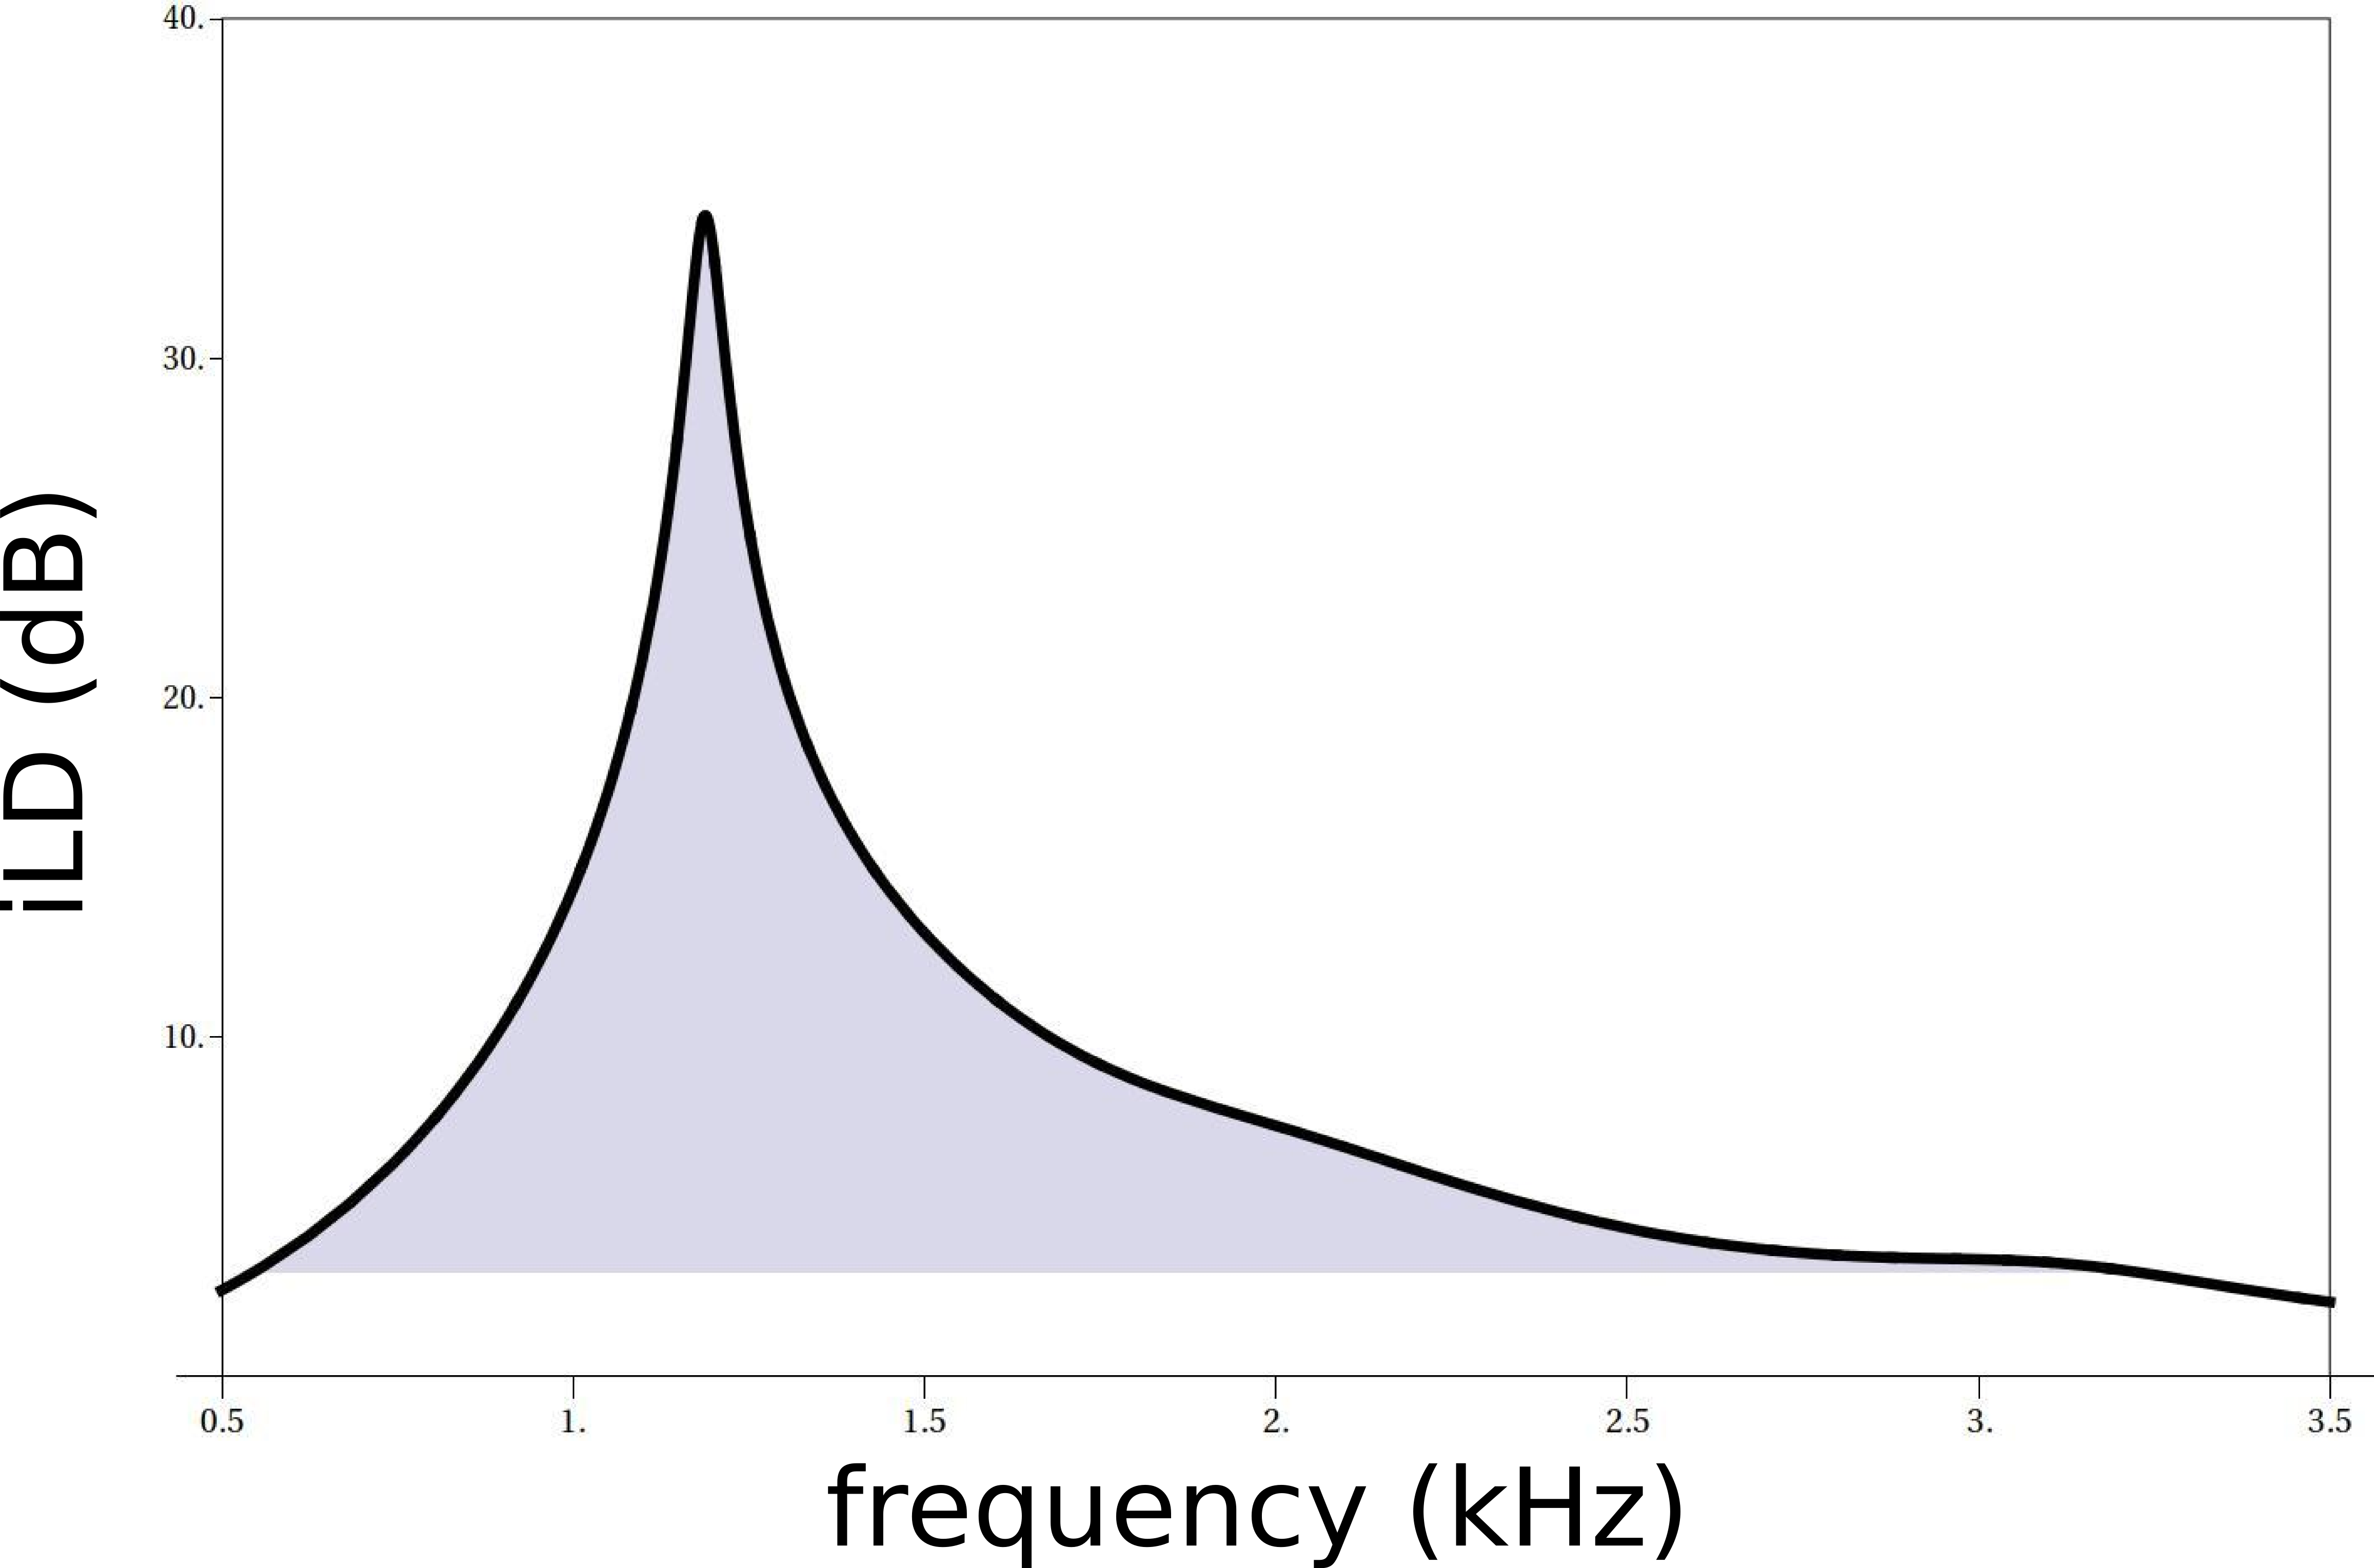
\includegraphics[width = 6 cm]{Diagrams/Presentation/iLDspectrum.png}
\begin{exampleblock}{}
\small
 \begin{itemize}
  \item iLD is a better cue at higher frequencies.
  \item Peak response at $\sim f_0\sqrt{1+1/4Q^2}$.
 \end{itemize}
\end{exampleblock}
\end{column}
     \begin{column}{0.5\textwidth}
     \flushright
 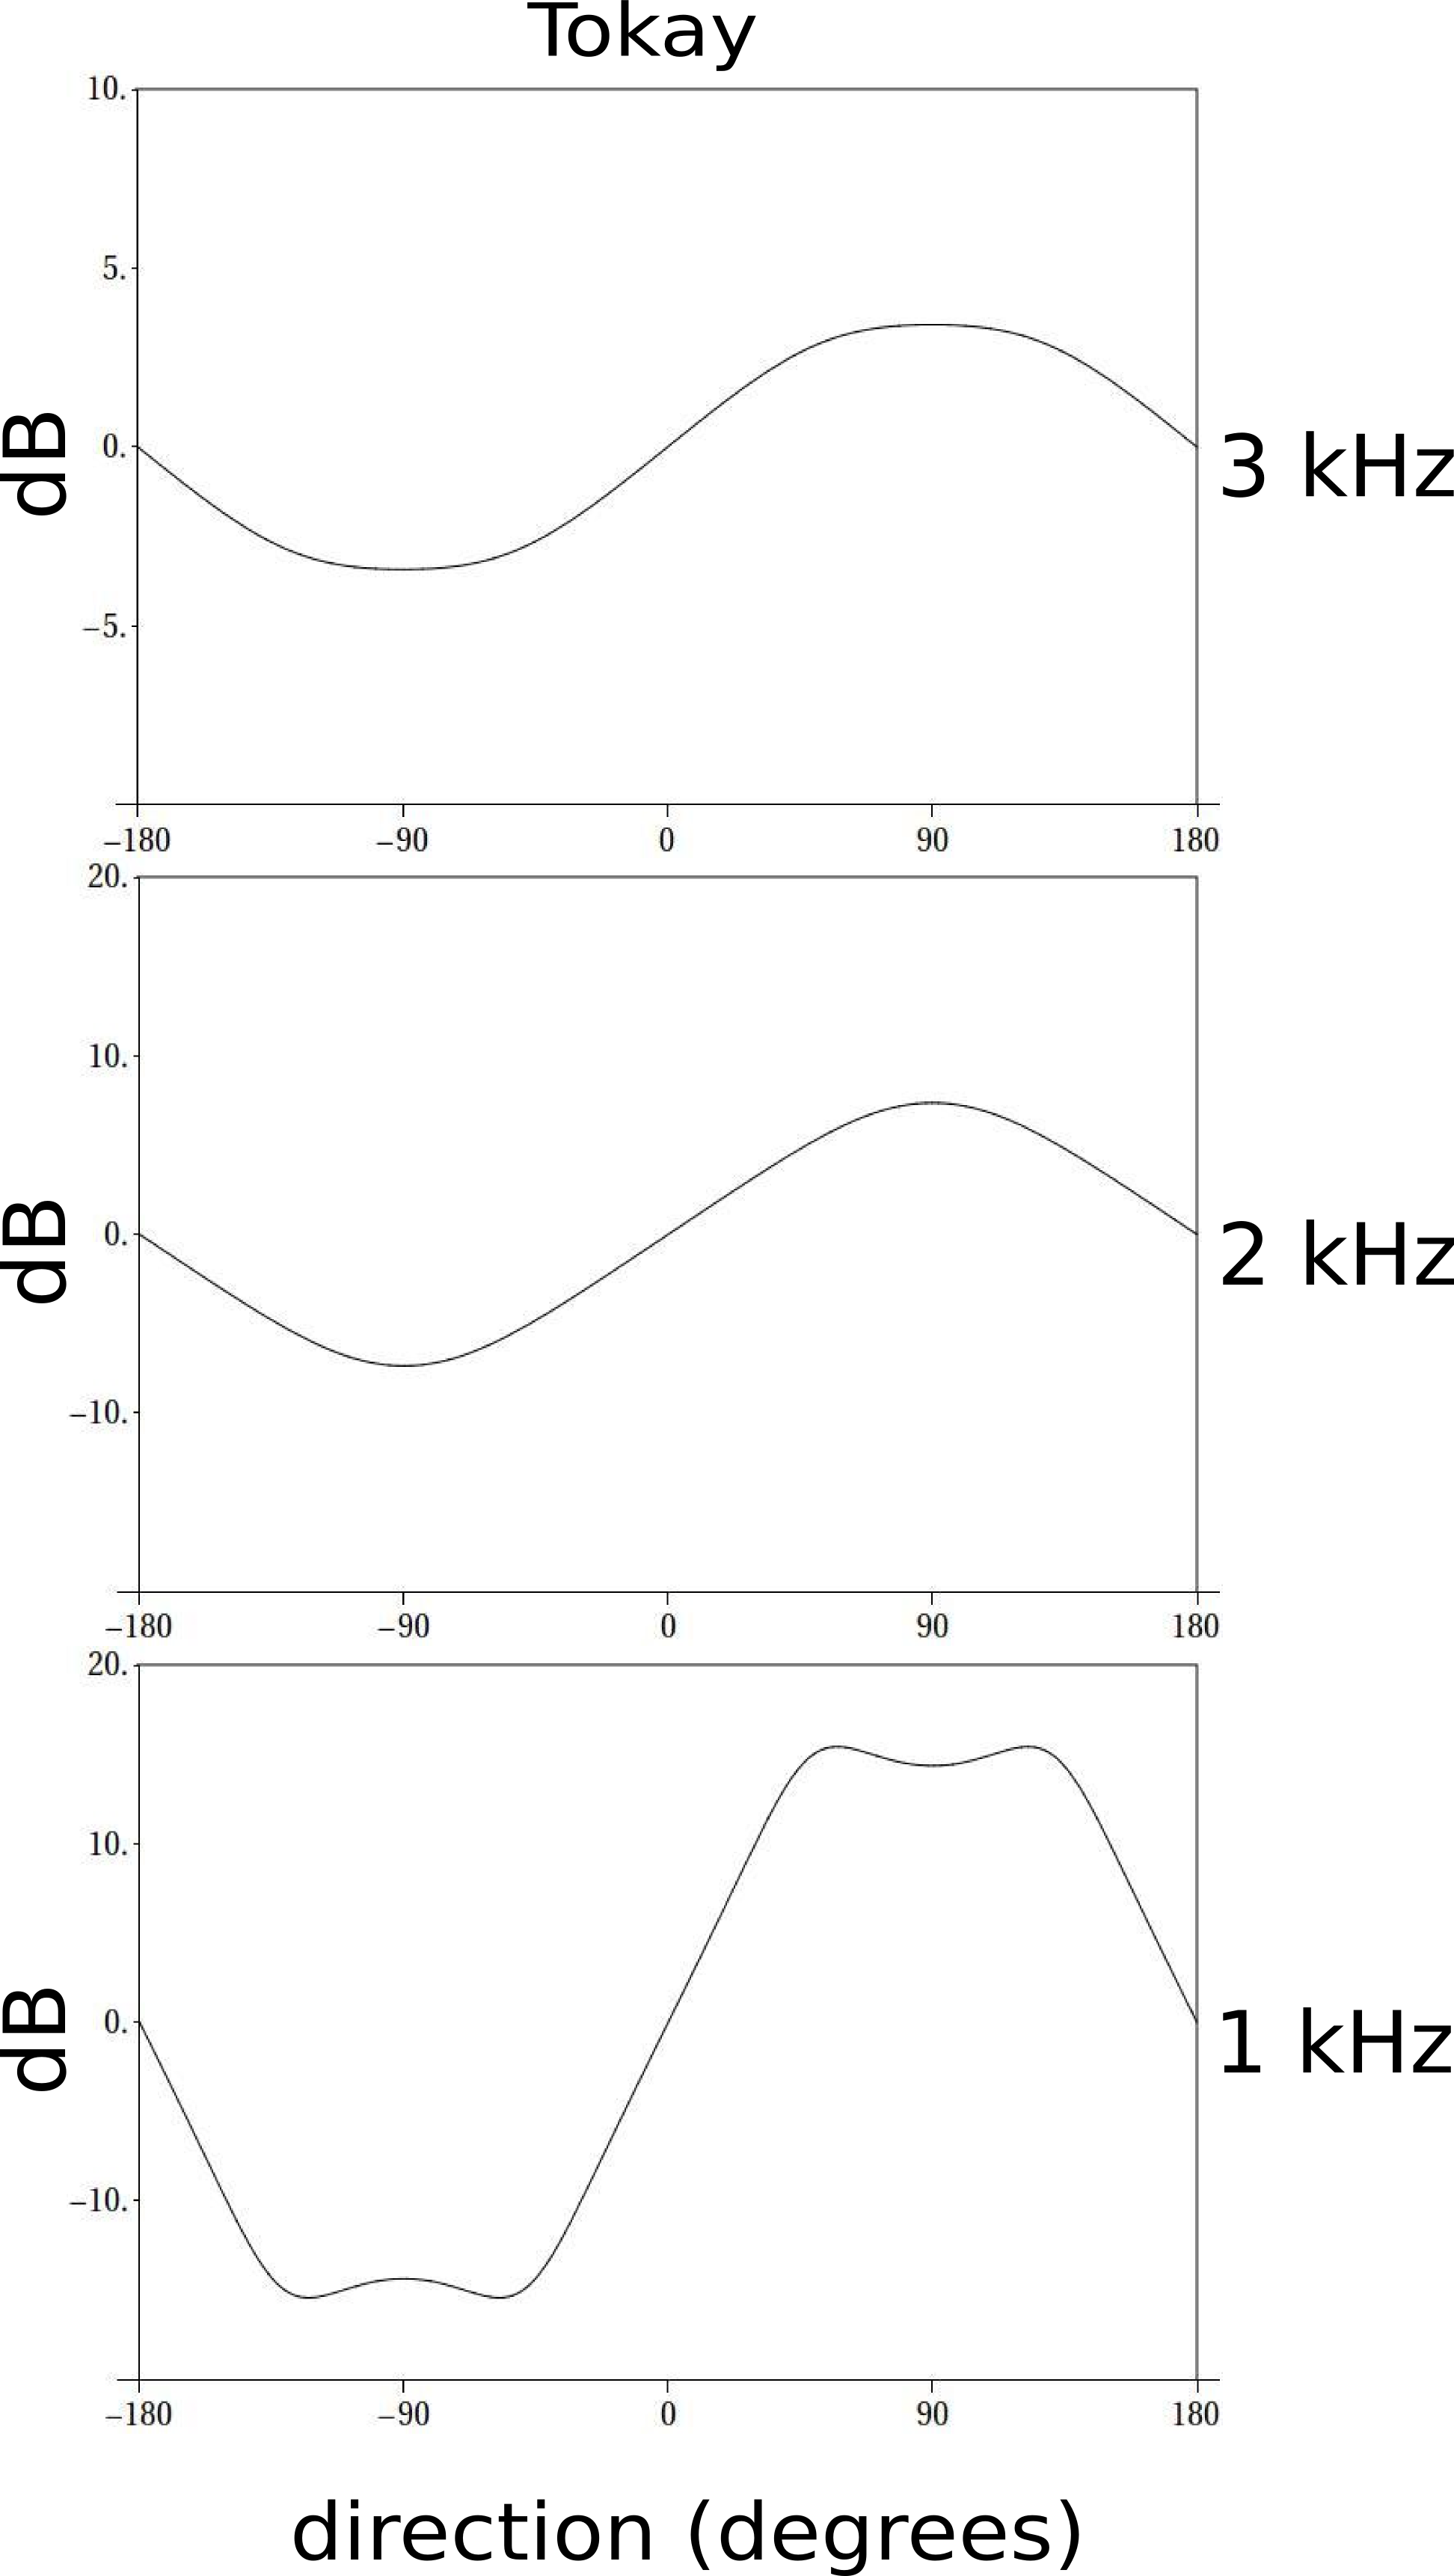
\includegraphics[width = 3.6 cm]{Diagrams/Presentation/iLDdirection.png}
\end{column}
\end{columns}
\end{frame}

\subsubsection{Internal Time Difference}
\begin{frame}[t]
\frametitle{iTD Frequency/Direction Dependence}
%\noindent iTD Spectrum and Direction Dependence
\begin{columns}
\begin{column}{0.5\textwidth}
 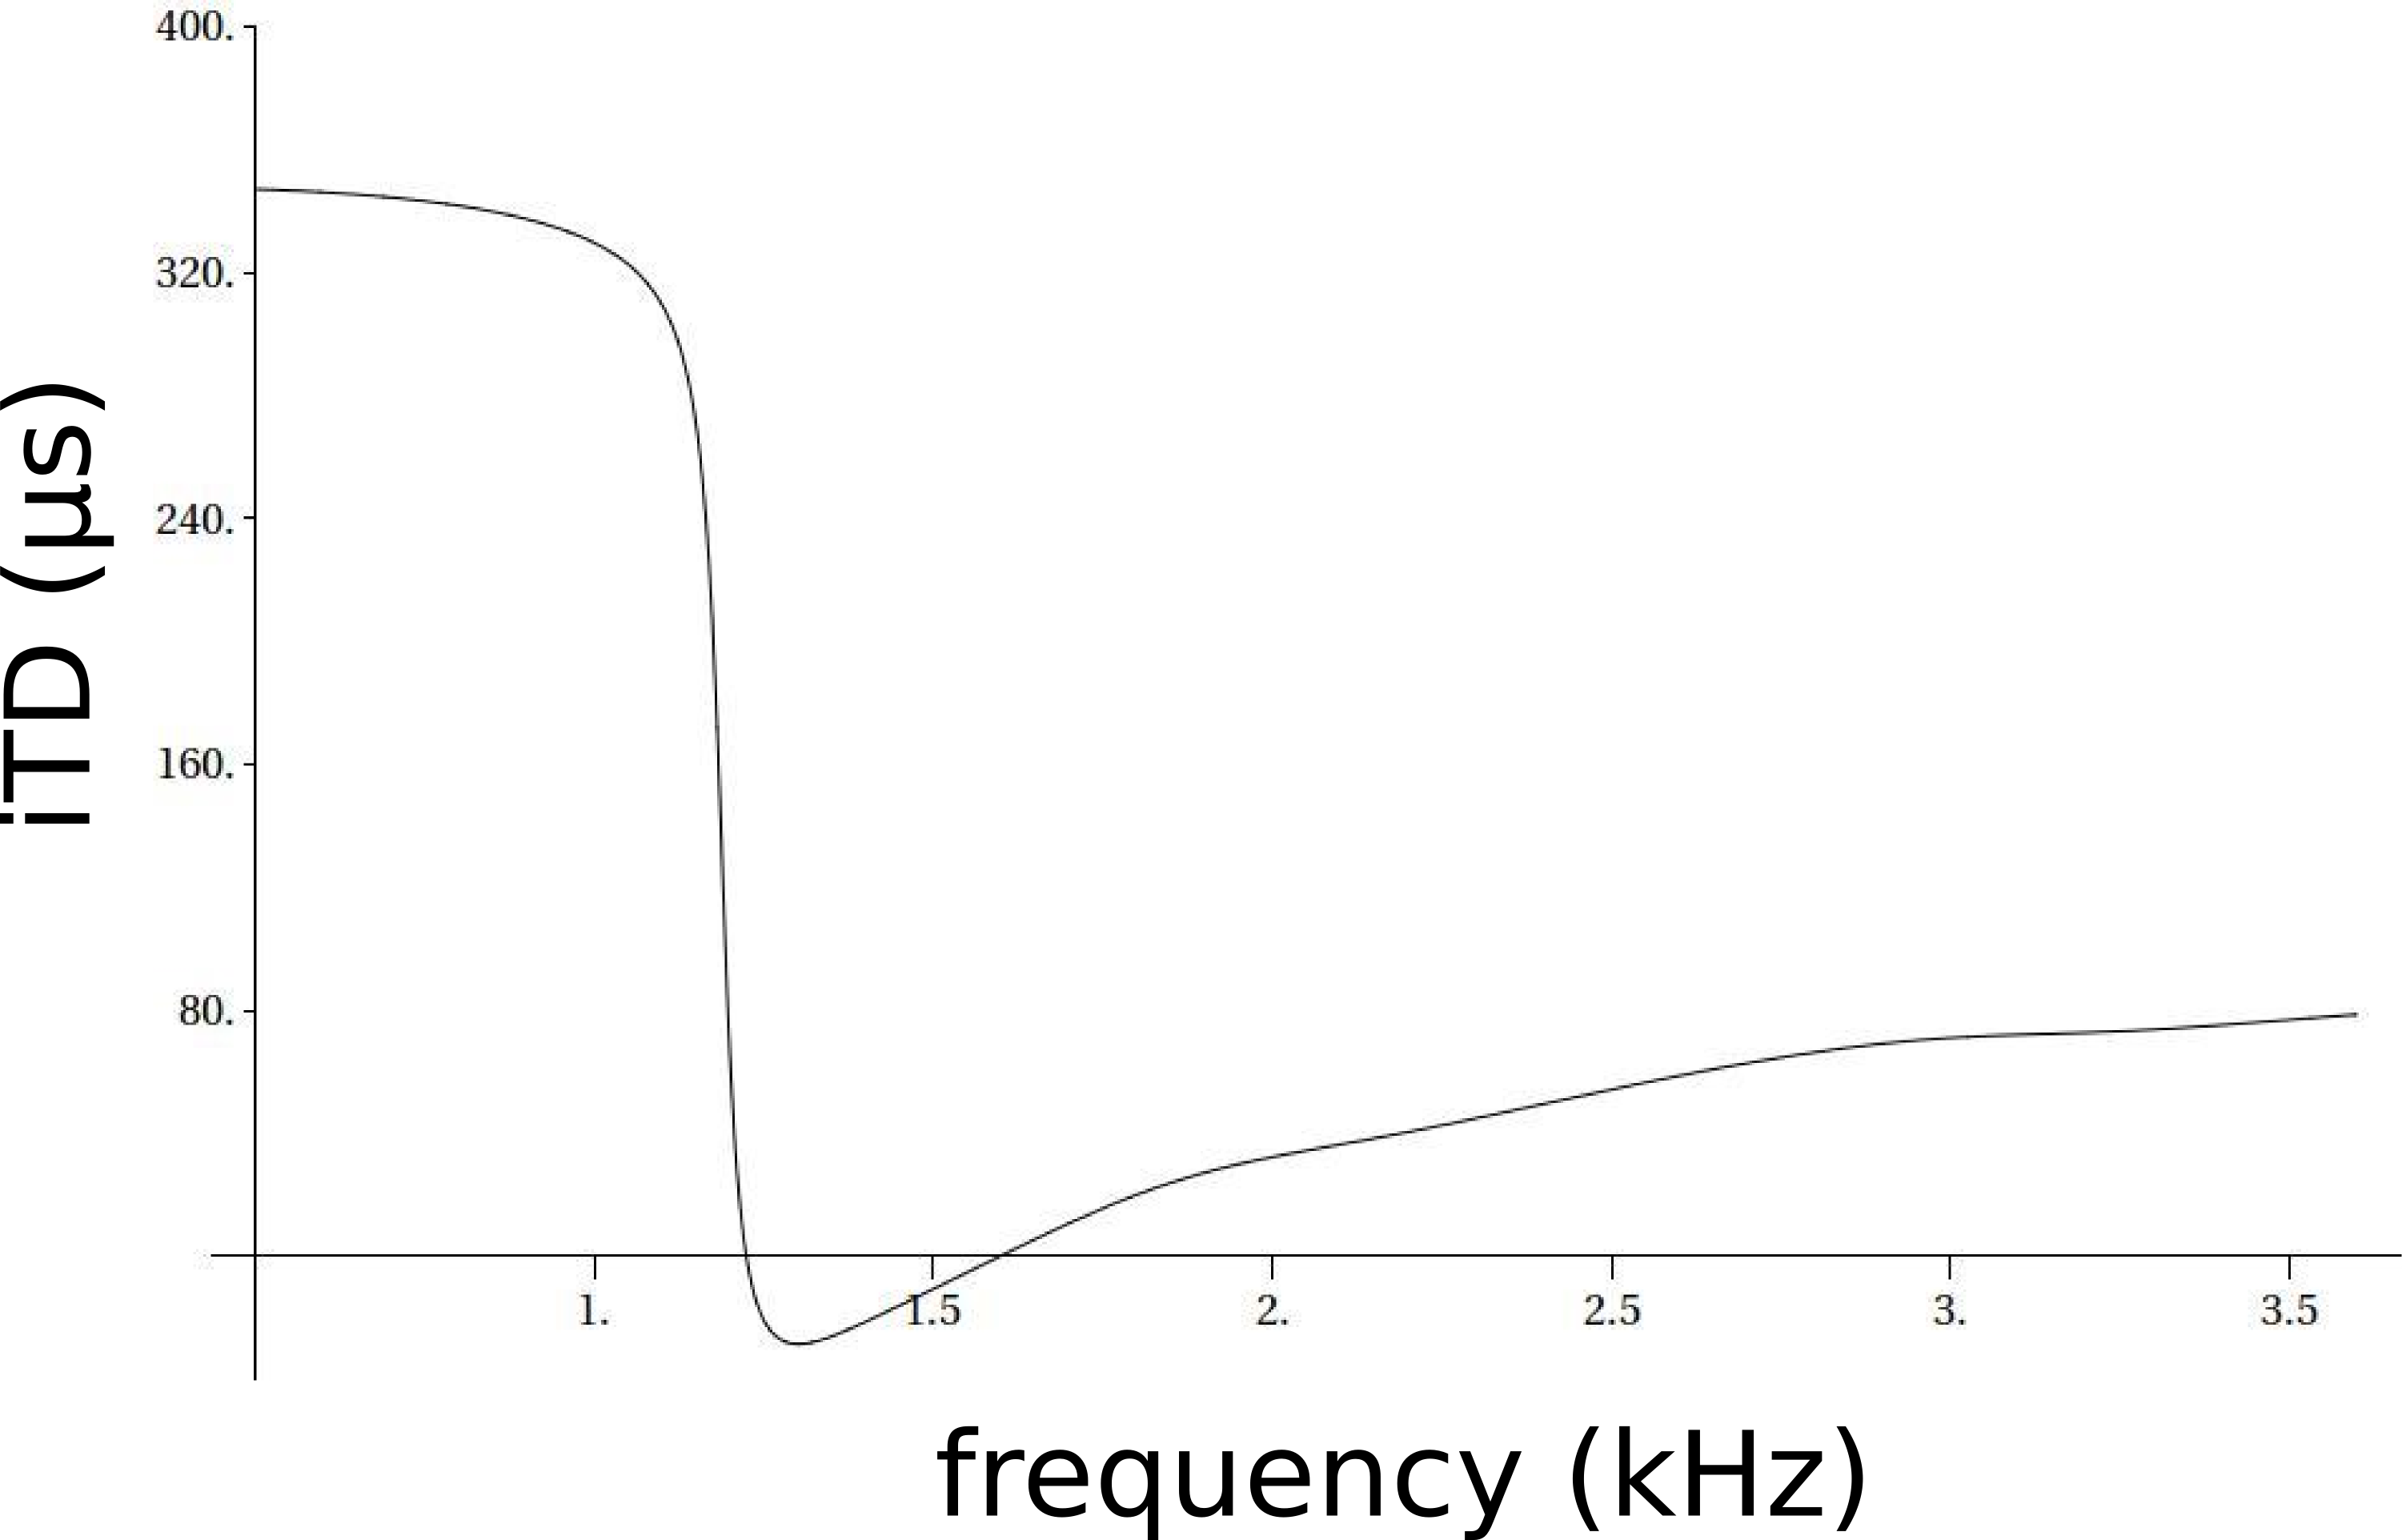
\includegraphics[width = 6 cm]{Diagrams/Presentation/iTDspectrum.png}
\begin{exampleblock}{}
\small
 \begin{itemize}
  \item iTD is a better cue at lower frequencies.
  \item constant up to $\sim f_0$.
  \item iTD $\approx  3\times$ITD
 \end{itemize}
\end{exampleblock}
\end{column}
     \begin{column}{0.5\textwidth}
     \flushright
 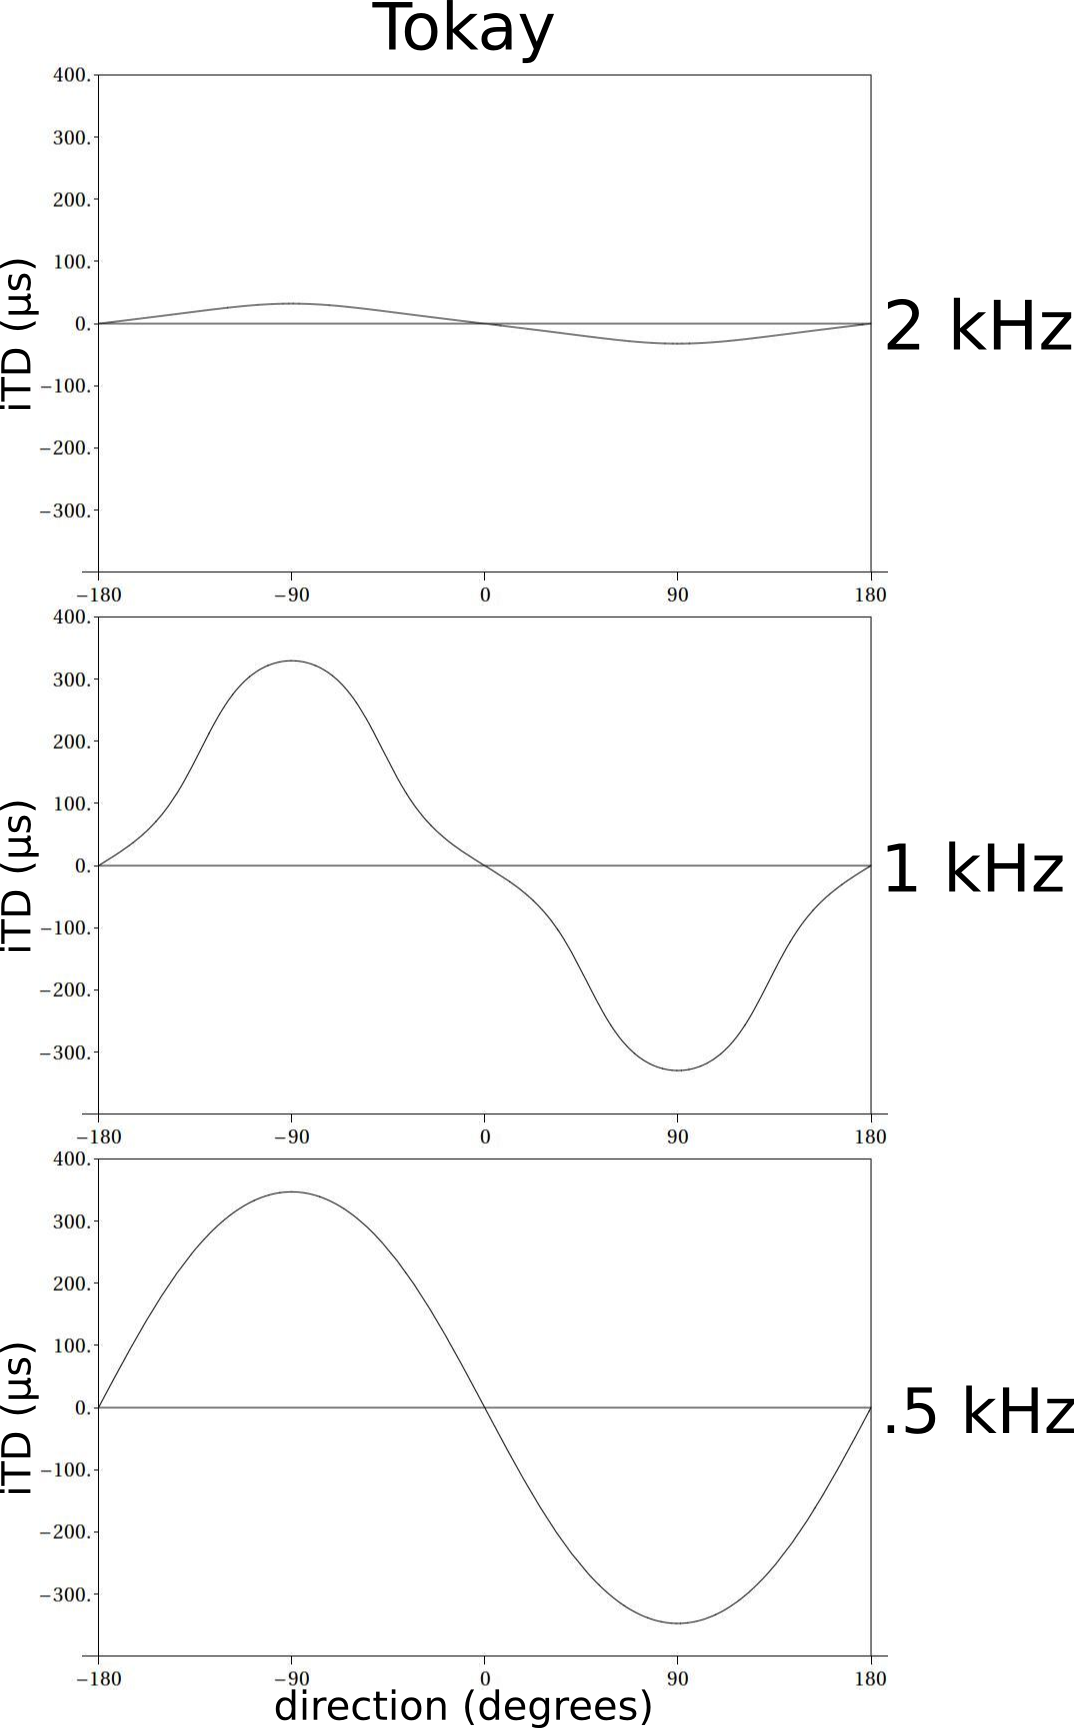
\includegraphics[width = 3.8 cm]{Diagrams/Presentation/iTDdirection.png}
\end{column}
\end{columns}
\end{frame}


\begin{frame}
\frametitle{iTD/iLD Frequency Regimes}
\begin{columns}
\begin{column}{0.5\textwidth}
\begin{exampleblock}{}
\small
 \begin{itemize}
 \item Presence of phase and amplitude sensitive neurons.
  \item Transition-frequency determined by $f_0,\ \alpha$. NOT by inputs.
  \item Possibile regime where both cues can simultaneously be used.
 \end{itemize}
\end{exampleblock}
\end{column}
     \begin{column}{0.5\textwidth}
      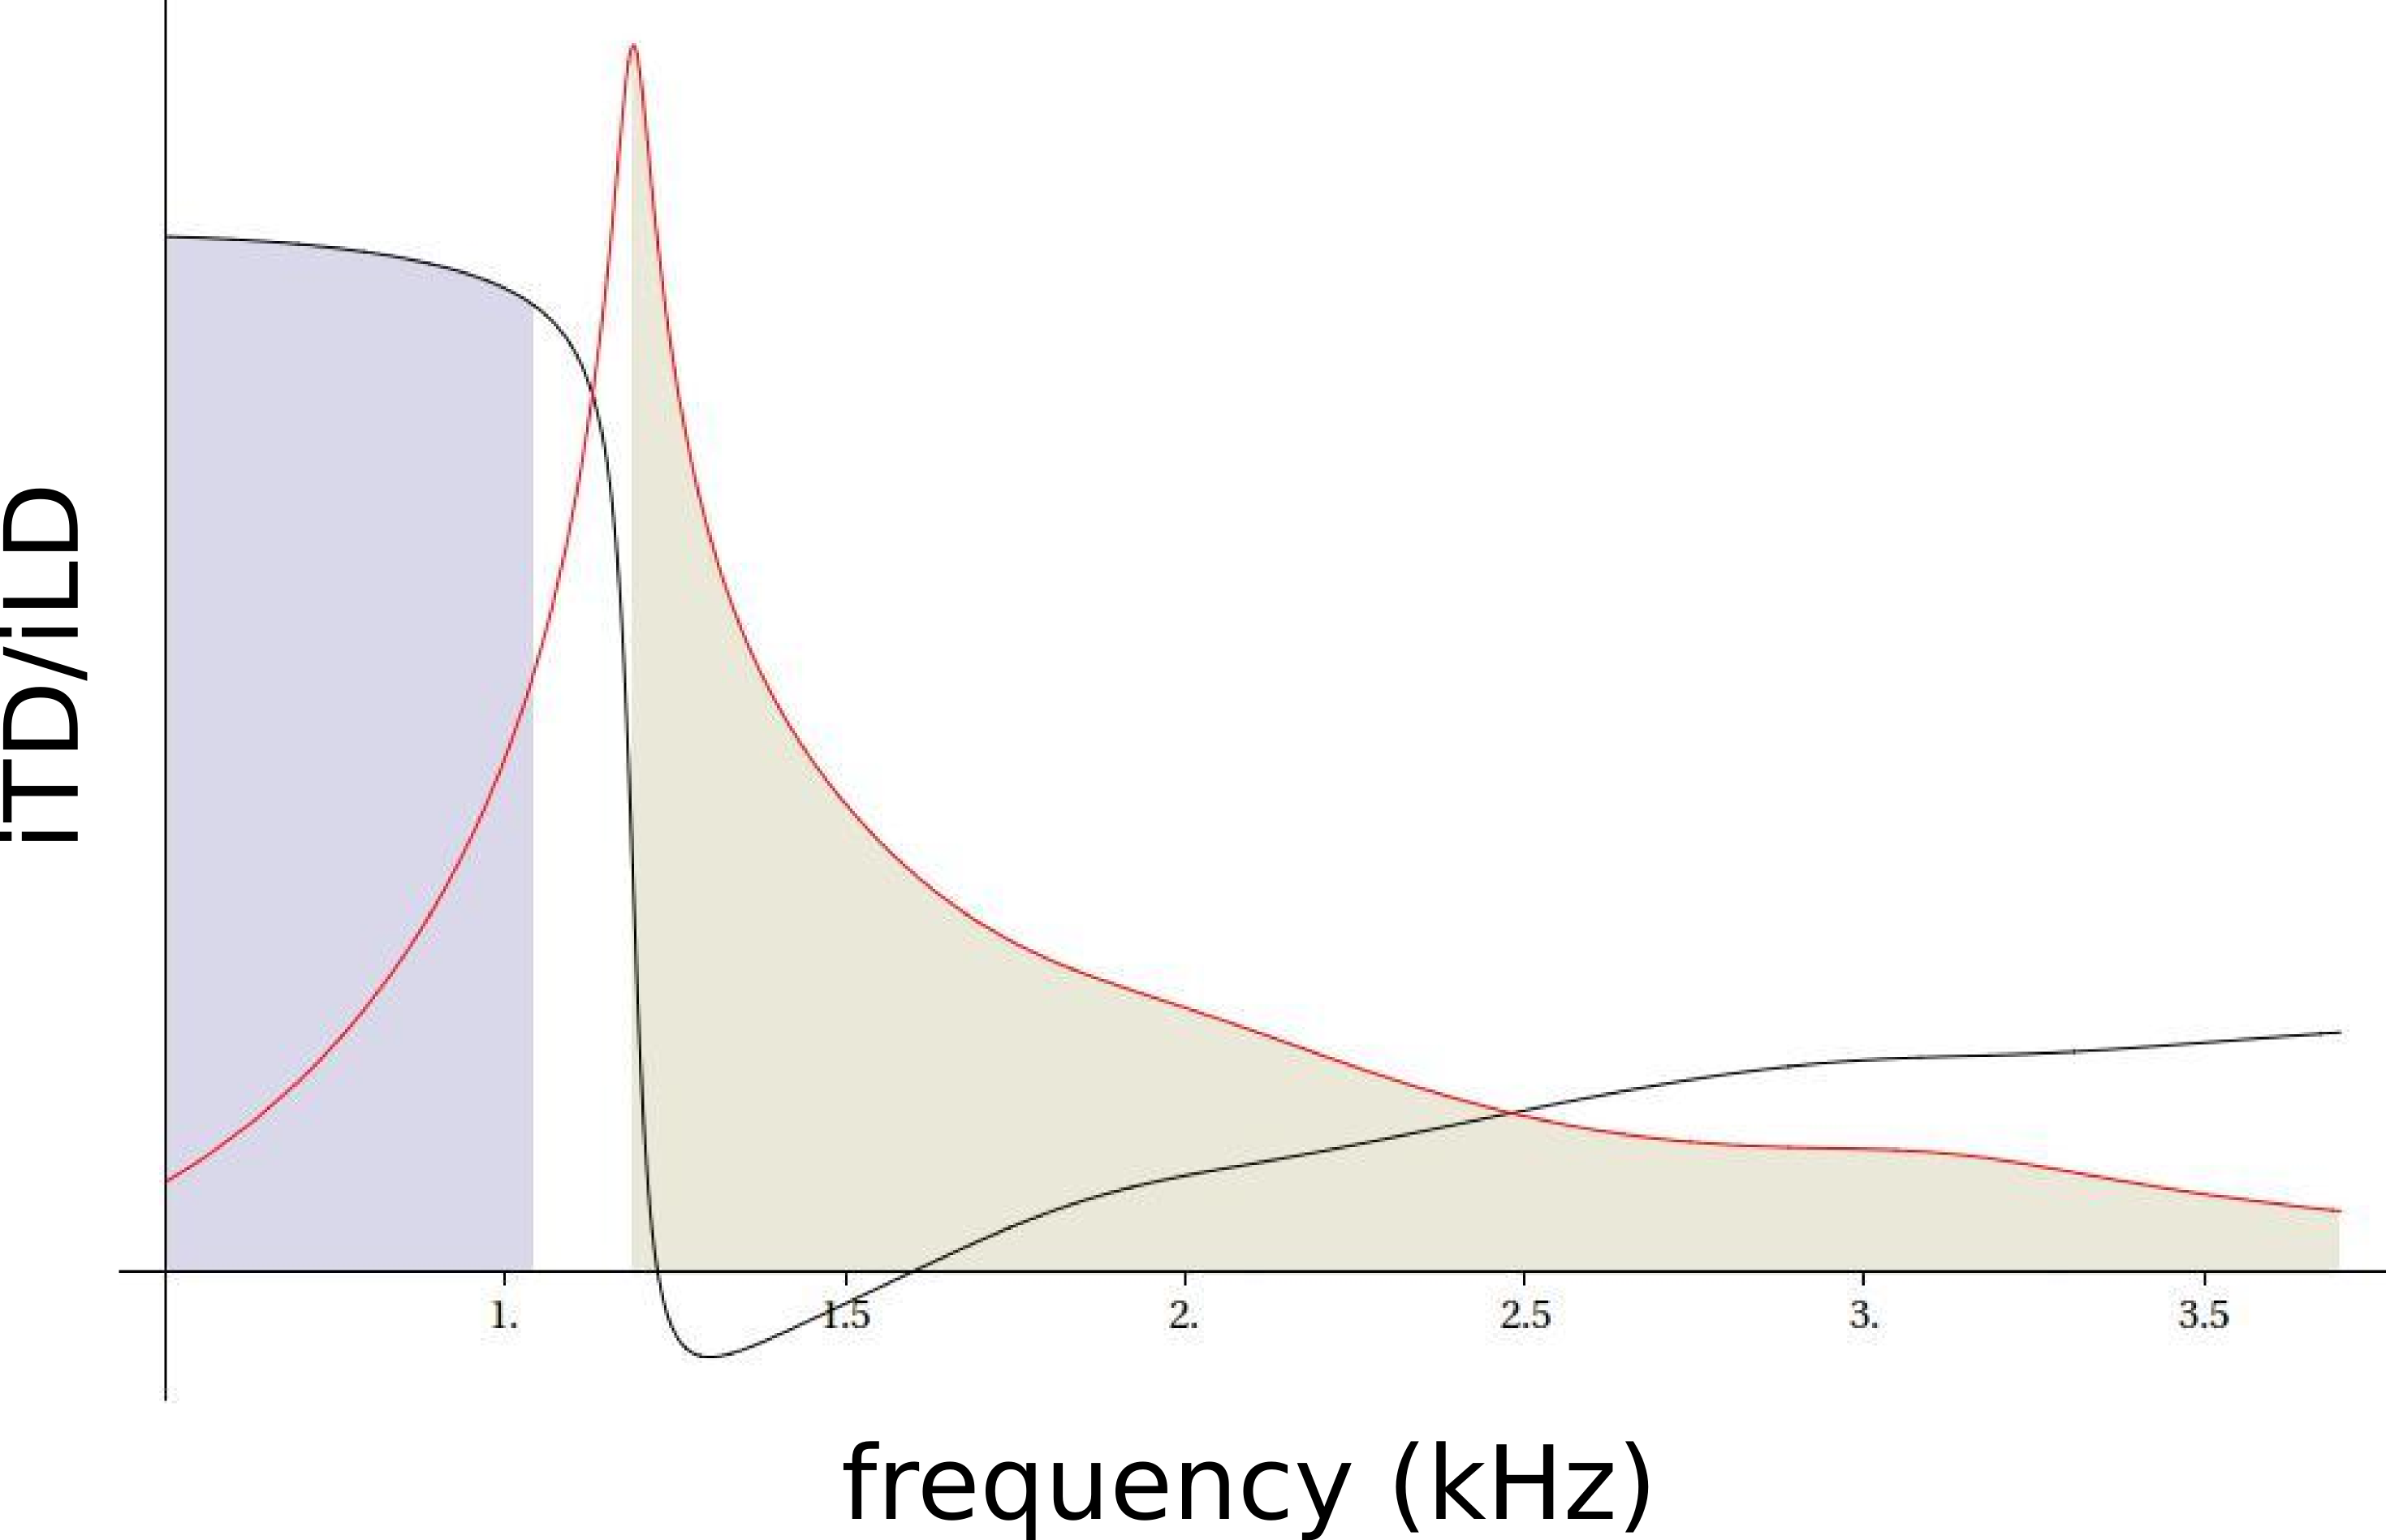
\includegraphics[width = 6 cm]{Diagrams/Presentation/tokayregions.png}
\end{column}
\end{columns}
\end{frame}

\section{Conclusion}
\begin{frame}[t]
 \frametitle{Conclusion}
 \begin{columns}
  \begin{column}{.4\textwidth}
 \onslide<1>{\begin{exampleblock}{}
 \begin{itemize}
  \item Single description for both regimes.
  \item Transition determined by $f_0$, $\alpha$.
 \end{itemize}
\end{exampleblock}}

 \onslide<2>{\begin{exampleblock}{Future Work}
 \begin{itemize}
  \item Extracolumella motion.
  \item Crocodiles 
  \begin{itemize}
  \item Independent above water.
  \item ICE underwater.
  \end{itemize}
 \end{itemize}
\end{exampleblock}}
\end{column}
\begin{column}{.6\textwidth}
\flushright
      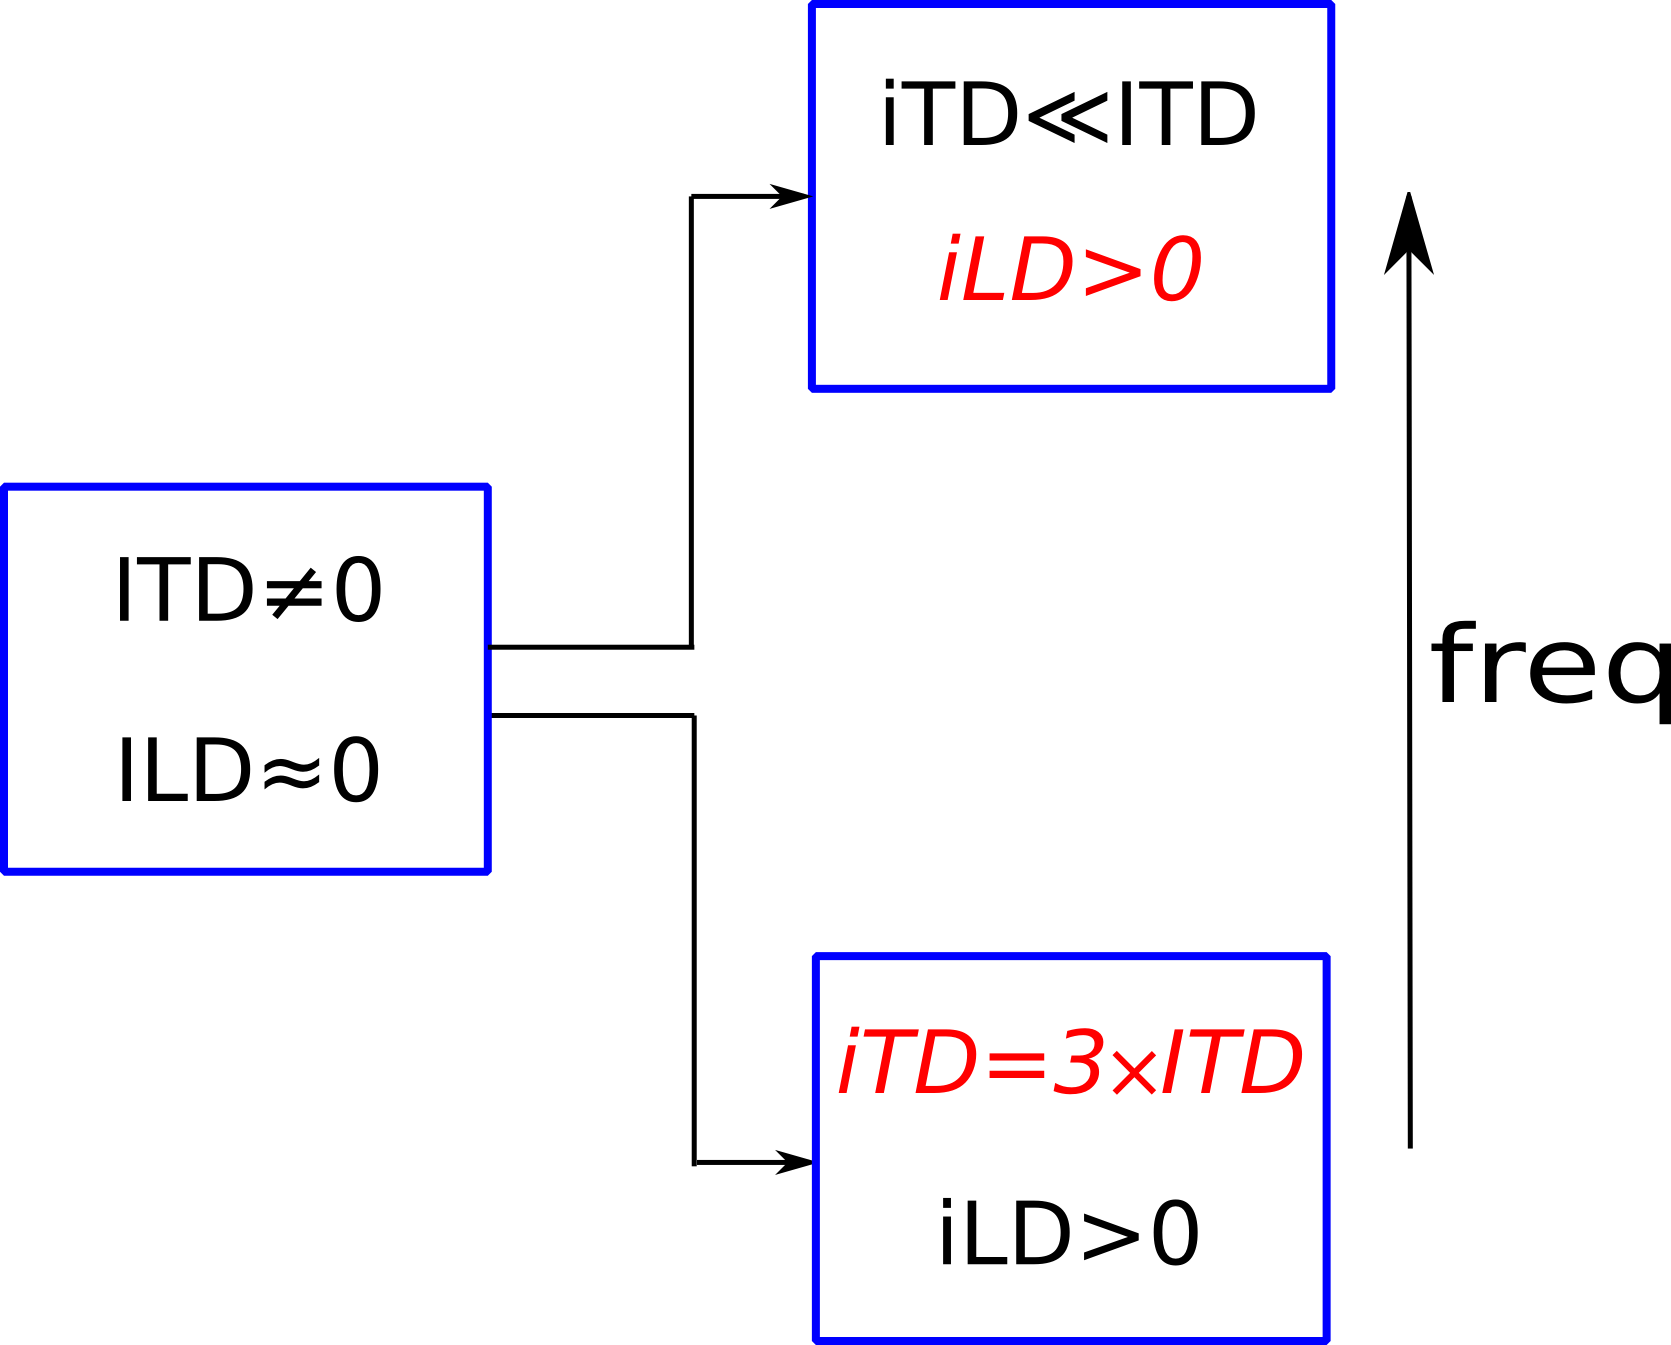
\includegraphics[width = 6 cm]{Diagrams/Presentation/conclusion1.png}
\end{column}

\end{columns}
\end{frame}

\begin{frame}[t]
 \frametitle{Thank You}
 \begin{figure}
  \centering
  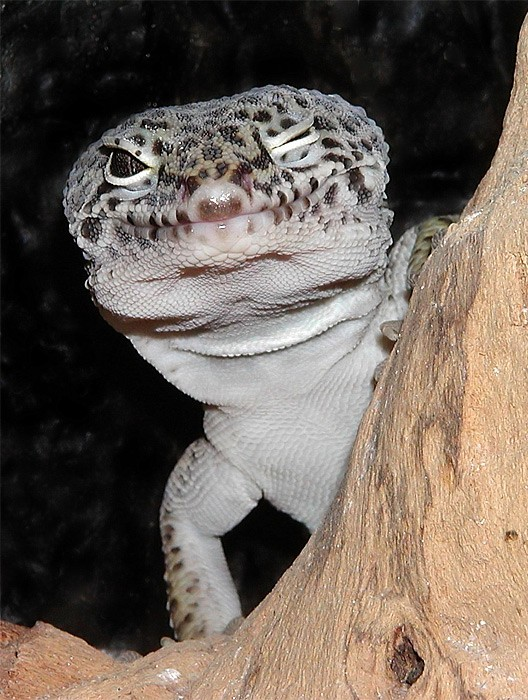
\includegraphics[width=.3\textwidth]{Diagrams/geckowink.jpg}
 \end{figure}
\end{frame}


\end{document}
